\documentclass[11pt,letterpaper,oneside]{book}
\usepackage[top=1.in, bottom=1in, left=1.in, right=1in, footskip=0.25in]{geometry}


% here, we pull in three useful commands from the book class into the article class
% since this is a book we dont need them tho

% allows a supplement to be made
\newcommand{\beginsupplement}{%
         \setcounter{table}{0}
         \renewcommand{\thetable}{S\arabic{table}}%
         \setcounter{figure}{0}
         \renewcommand{\thefigure}{S\arabic{figure}}%
         \setcounter{section}{0}
         \renewcommand{\thesection}{S\arabic{section}}
     }
      


% useful splitcell command for tables that have big entries
\newcommand{\splitcell}[2][c]{%
  \begin{tabular}[#1]{@{}l@{}}#2\end{tabular}}


  \usepackage{ccaption}
  \usepackage{afterpage}
\usepackage{fancyhdr}

\fancypagestyle{frontmatter}{%
  \renewcommand{\headrulewidth}{0pt}% No header rule
  \renewcommand{\footrulewidth}{0pt}% No footer rule
  \fancyhf{}% Clear header/footer
  \fancyfoot[C]{\thepage}%
}

\fancypagestyle{mainmatter}{%
  \doublespace
  \renewcommand{\headrulewidth}{0.4pt}% header rule
  \fancyhf{}
  \fancyhead[L]{\itshape\nouppercase{\leftmark}}
  \fancyfoot[C]{\thepage}
}

\usepackage{ragged2e}
\setlength{\RaggedRightParfillskip}{.25\textwidth plus 1fil}
\setlength{\RaggedRightRightskip}{0pt plus .1\textwidth}
\setlength{\RaggedRightParindent}{1em}

\usepackage[font=rm, labelfont={rm,bf}, margin=0.3in]{caption}
\usepackage{subcaption}
\usepackage[T1]{fontenc}
\usepackage{textcomp}
\usepackage[english]{babel}
\usepackage[utf8x]{inputenc}
\usepackage[sc]{mathpazo}
\usepackage{helvet}
\usepackage{amsmath,amssymb,amsfonts,mathrsfs,mathtools,subeqnarray}
\usepackage{graphicx}
\usepackage[sort&compress,comma,numbers]{natbib}
\usepackage{setspace}
\usepackage{titling}
\usepackage{bibentry}
\usepackage[plain]{fancyref}
\usepackage[linktoc=all]{hyperref}
\hypersetup{
    colorlinks,
    citecolor=black,
    filecolor=black,
    linkcolor=black,
    urlcolor=black
}

% for chapter on MPC design
\usepackage{amsthm}
\theoremstyle{asm}
\newtheorem{asm}{Assumption}

\theoremstyle{plain}% default
\newtheorem{thm}{Theorem}
\newtheorem{cor}{Corollary}
\newtheorem{defn}{Definition}
\theoremstyle{remark}
\newtheorem*{rmk}{Remark}
\renewcommand{\qedsymbol}{$\blacksquare$}

\newcommand\floor[1]{\lfloor#1\rfloor} \newcommand\ceil[1]{\lceil#1\rceil}

% For figure captions
%\usepackage[font=rm]{caption}
%\providecommand{\titlecaption}[2]{\caption[#1]{{\small \rmfamily{ #1.}}\small #2}}

% Make subsections more clear
\usepackage{titlesec}

%\titleformat{\part}[display]
%  {\normalfont\sffamily\huge\bfseries}
%  {\partname\ \thepart:}{16pt}{\Huge}
\titleformat{\chapter}[display]
  {\normalfont\rmfamily\Large\bfseries}
  {\chaptertitlename\ \thechapter}{12pt}{\Large}
\titleformat{\section}
  {\normalfont\rmfamily\Large\bfseries}
  {\thesection}{1em}{}

\titleformat{\subsubsection}
  {\rmfamily\itshape\bfseries}{\thesubsubsection}{1em}{}

% Imports/macros for chapter 2
\usepackage{booktabs}
% \usepackage{chemarr}
\usepackage{longtable}

% define the imaginary number
\renewcommand{\j}{\mathrm{i}}

%
%
% for use in python
\usepackage[procnames]{listings}
\usepackage{color}
 
\definecolor{keywords}{RGB}{255,0,90}
\definecolor{comments}{RGB}{0,0,113}
\definecolor{red}{RGB}{160,0,0}
\definecolor{green}{RGB}{0,150,0}
 
\lstset{language=Python, 
        basicstyle=\ttfamily\scriptsize, 
        keywordstyle=\color{keywords},
        commentstyle=\color{comments},
        stringstyle=\color{red},
        showstringspaces=false,
        identifierstyle=\color{green},
        procnamekeys={def,class}
}
% for python END
%
%

\newcommand\blfootnote[1]{%
  \begingroup
  \renewcommand\thefootnote{}\footnote{#1}%
  \addtocounter{footnote}{-1}%
  \endgroup
}

% for intro
\usepackage{bm}

% Imports for chapter 5
\usepackage{nicefrac}
\usepackage{supertabular}

% For model float
\usepackage{float}
\newfloat{model}{thp}{lop} % Frank doesn't want models labeled by chapter
\floatname{model}{Model}
\floatstyle{plaintop}
\restylefloat{model}

% For list of models in the preamble
% \usepackage{scrhack} % load after "float"

\newcommand*{\fancyrefmodlabelprefix}{mod}

\fancyrefaddcaptions{english}{%
  \providecommand*{\frefmodname}{model}%
  \providecommand*{\Frefmodname}{Model}%
}

\frefformat{plain}{\fancyrefmodlabelprefix}{\frefmodname\fancyrefdefaultspacing#1}
\Frefformat{plain}{\fancyrefmodlabelprefix}{\Frefmodname\fancyrefdefaultspacing#1}

\frefformat{vario}{\fancyrefmodlabelprefix}{%
  \frefmodname\fancyrefdefaultspacing#1#3%
}
\Frefformat{vario}{\fancyrefmodlabelprefix}{%
  \Frefmodname\fancyrefdefaultspacing#1#3%
}

\title{A Computational Approach to Analysis and Control\\of the Mammalian Circadian Oscillator}

% This command is great to only print out a certain chapter, keeping references etc from other chapters.
%\includeonly{chap6/future}

\begin{document}
\sloppy % somewhat counter-intuitively, this makes latex respect the page margins more rigorously.
\doublespace
\frontmatter
\pagestyle{frontmatter}
\thispagestyle{empty}
\begin{center}

  \vfil
  {\large\thetitle}\\
  \vfil
  A dissertation presented\\
  by\\
  John H. Abel\\
  to\\
  The Department of Systems Biology\\
  \vfil
  in partial fulfillment of the requirements\\
  for the degree of\\
  Doctor of Philosophy\\
  in the subject of\\
  Systems Biology\\
  \vfil
  Harvard University\\
  Cambridge, Massachusetts
  \vfil
  April 2018
\end{center}

\chapter*{}
\null
\thispagestyle{empty}
\vfill
\begin{center}
  \copyright \ 2018 John H. Abel\\
  All rights reserved.
\end{center}


\include{preamble/abstract}



{\singlespace
\tableofcontents
}
\chapter*{Acknowledgement}
\markboth{Acknowledgement}{Acknowledgement}


\singlespace{I owe such an intellectual debt to so many individuals that it feels like the true author list for this dissertation should be half its content.
Most prominently I would like to thank my primary advisor Frank Doyle for his unwavering support during this process. 
It's only in retrospect that I can understand how valuable your contributions were to the development of my thinking.
To my coadvisors, Professors Linda Petzold and Beth Klerman, and my additional mentors Professors Erik Herzog and Hyunmin Yi: thank you for committing your time and intellectual energy to my development.
Sorry for the late hours at which I replied to your emails.
I've also been quite lucky to have a remarkable cast of collaborators, and I would like to thank Vania Carmona-Alcocer, Ankush Chakrabarty, Brian Drawert, Daniel Granados-Fuentes, Cristina Mazuski, Peter St.\ John, and Steffen Waldherr.
I'm humbled to be considered your peer.
In particular, Peter St.\ John's mentorship has had a disproportionate positive effect on my research, and for that I am grateful.
I am also grateful for the community that the entire Doyle group has been throughout my time in it.
From squash, to ill-advised witch hunts (apologies to Lindsey Brown, no apologies to Kelsey Dean), to Thanksgivings at Eyal's, it's been a remarkable time.
Thank you especially to Alejandro Laguna, Kelsey Dean, Faith Barcelo, Eyal Dassau, Sunil Deshpande, Joon Bok Lee, Ravi Gondhalekar, and Gunjan Thakur for moving across the country with me.


I have been extraordinarily privileged to have had the support of numerous educators and institutions, all of which contributed to my completion of this dissertation.
Harvard, UC Santa Barbara, and Tufts have been fantastic developmental environments to which I hope to return frequently.
To Liz Pomerantz and Sam Reed: I could not have survived here without your help, and the Systems Biology program has felt like an intellectual home ever since I arrived on campus.
Finally, I would like to thank the educators who inspired me to embrace challenging questions from early on, especially Matthew McDonough, Thomas Morey, and Sr.\ Carol Ann Murray.

To my family
\{Anthony, Frederick, Joseph, Judy, Katrina, Virginia\} Abel, \{Faith, Kim\} Blake, \{Alyssa, Mary\} Miller:
thank you for making me who I am. I hope I have made you proud.
I would like to especially acknowledge Faith Blake for her often unnoted intellectual contributions to my work, most prominently in interpreting data recorded from the fetal suprachiasmatic nucleus and in editing and questioning every manuscript I have written.
It seemed out of place to acknowledge you on the papers, in that all of my ideas were also fundamentally yours.
I hope that I can contribute to your career even half of what you have to mine.
I would also like to thank my friends, but in lieu of listing names I'll list locations significant to us: Beacon Hill, Big Sur, Hemenway, Holualoa, Indio, Isla Vista, the Louvre, West End Avenue, Winthrop.
}


\include{preamble/quote}

\mainmatter
\pagestyle{mainmatter}

\chapter{Introduction}
\blfootnote{Portions of this chapter appear as
J.H.\ Abel and F.J.\ Doyle III, ``A systems approach to analysis and control of mammalian circadian dynamics,'' \textit{Chemical Engineering Research and Design}, vol.~116, 2016. DOI:~10.1016/j.cherd.2016.09.033; and J.H.\ Abel, A.\ Chakrabarty, and F.J.\ Doyle~III ``Pharmaceutical-based entrainment of circadian phase via nonlinear model predictive control,'' submitted.
The text has been modified to provide a more thorough introduction.
% copyright info covered under personal use: https://www.elsevier.com/about/our-business/policies/copyright/personal-use
% double checked using get rights and content - all good
}

Circadian rhythms are endogenous oscillations in gene expression, metabolism, and behavior that allow an organism to adjust its internal state to predictable cyclic changes in the environment.
This advantageous feed-forward approach to life in a temporally cyclic environment allows an organism with a circadian rhythm to anticipate environmental variability and adjust its physiology without a time lag.
Circadian regulation of biological processes is therefore highly-conserved: these rhythms have been identified in diverse species from mammals, insects, plants, and fungi to prokaryotic cyanobacteria \cite{Reppert2002, Hardin2005, Harmer2000, Dunlap2004a}.
Although circadian clocks share common properties between species, the mechanistic origins and hierarchical complexity of these rhythms can vary significantly.
Prokaryotes have been shown to use minimal phosphorylation-based nontranscriptional oscillators, which may be reconstituted \textit{in vitro} \cite{Ishiura1998, Nakajima2005}.
Meanwhile, eukaryotic organisms employ transcriptional-translational feedback loops in addition to post-translational protein modification for timekeeping \cite{Dunlap1999, ONeill2011}.
In larger organisms such as mammals, circadian rhythms must be coordinated across cells and tissues, resulting in a complex yet robust circadian control system \cite{Welsh2010, Doyle2006}.
% end paragraph, talk about approaches

The inherently complex (i.e.\ involving nonlinearity and feedback) and stochastic (i.e.\ fundamentally involving randomness and noise) nature of these processes has necessitated mathematical approaches for understanding biological clocks, as their properties emerge from the often-imprecise interaction of numerous molecules and pathways.
Such approaches have included mechanistic and empirical process modeling \cite{Kronauer1999, Jewett1999, Leloup2003a, Gonze2003, Forger2005, To2007, Mirsky2009b,  Ko2010, Hirota2012a}, robustness and sensitivity analysis \cite{Leloup2003a, Gonze2006, Rougemont2007, Taylor2008a, Tidor2009, StJohn2013, Taylor2014a}, and optimal or feedback control \cite{Doyle2006, Bagheri2008, Bagheri2008a, Serkh2014, Zhang2016}.
%cite models, methods, tools, etc. essentially show that this is true here
This thesis presents recent advances in developing an understanding of, and artificially exerting control over, the mammalian circadian system through mathematical approaches.


\subsubsection*{On organization}
In this chapter, I begin by presenting a brief historical overview of the study of daily patterns of behavior, culminating with the identification of clock genes in multiple organisms in the 1990s.
I next define the general characteristics that constitute a circadian rhythm.
I then introduce biological generation of mammalian circadian rhythms, and also note how this structure compares to that of other organisms.
I present a mathematical framework for modeling and analysis of circadian dynamics based on the limit cycle oscillator, and present derivations for relevant quantities.
Finally, I discuss motivation for feedback control of circadian rhythms, and the components of a system to achieve this.

The ensuing dissertation is then divided into two main sections to reflect the two foci of my research.
In Section I, I present projects in fundamental biology toward the aim of understanding the structure and function of mammalian circadian rhythm generation and synchronization in the suprachiasmatic nucleus (SCN).
In Section II, I present a mathematical framework for taking control of this system, and derive results that aim to guide the development of this capability.
Future research aims are included separately for each Section.

My exact contributions are noted for each section so as to avoid claiming credit for the work of my dedicated and highly skilled collaborators.
The majority of this work has already been published, and for published chapters I have attempted to edit as little as possible for this volume.
This serves two purposes: consistency in the literature record and avoiding the introduction of new errors of my own making.

\subsubsection*{On notation}

Where possible, I have generally attempted to adopt a uniform notation throughout this thesis.
This has primarily affected the presentation of this Introduction: the notation has been changed from the original publication to match with Section II.
For the confused reader, I would recommend studying the original publications in detail: the notation in these is certainly internally consistent and self-contained.

\section{An introduction to circadian rhythms}

\subsection*{A brief history of circadian biology}
It has long been noticed that organisms adjust their physiology in accordance with day-night cycles.
Androsthenes of Thasos, an admiral in the navy of Alexander the Great, noted daily rhythms in leaf movements of \textit{Tamarindus indicus}, but did not suspect that these rhythms were more than a response to light \cite{McClung2006b}.
It was not until the 1700s that the first ``true'' chronobiological experiment was performed, demonstrating that rhythms in leaf movement are endogenous, rather than a response to the light-dark cycle \cite{de1729observation}.
In the following 200 years, endogenous rhythms in physiology were observed in more plant species, arthropods \cite{kiesel1894untersuchungen}, and eventually, rats \cite{richter1922behavioristic}.
By the mid 20th century, it was well-established that an unidentified endogenous process was driving the near-24 hour rhythms in behavior observed under constant conditions.

Perhaps the most important discovery in identifying the underlying basis of circadian rhythms was the discovery of the \textit{Period} (\textit{Per}) gene in \textit{Drosophila melanogaster} in 1971 \cite{Konopka1971}.
In a classic work, Konopka and Benzer demonstrated that inducing mutations in a single gene on the \textit{Drosophila} X chromosome can induce lengthened, shortened, or abolished circadian eclosion rhythms in constant darkness.
Furthermore, these mutations conferred altered circadian period phenotypes in adults, indicating that an underlying genetic oscillator drives circadian rhythms, and that this oscillator persists through metamorphosis.
It was this and the ensuing studies that led to the discovery of the autoregulatory function of \textit{Per} \cite{Hardin1990}, the discovery of the gene involved in its nuclear localization (\textit{Timeless}) \cite{Vosshall1994}, and the 2017 Nobel Prize in Physiology or Medicine.
In this same timeframe, the genetic basis of the mammalian clock was identified as a transcription-translation feedback loop analogous to the \textit{Per}/\textit{Timeless} feedback loop of \textit{Drosophila}.
A homologous \textit{Per} gene was identified in mammals, and \textit{Cryptochrome} was identified as its co-regulator \cite{Vitaterna1999}.
Furthermore, homologs of the \textit{Clock} gene were identified as the transcriptional activator in both mammals and \textit{Drosophila} \cite{Vitaterna1994, Darlington1998}.

Since the identification of the key transcriptional pathways of the mammalian circadian clock, much effort has focused on elucidating the complex genetic architecture surrounding the clock \cite{Zhang2009, Takahashi2016}.
The circadian oscillator has been found to widely regulate transcription within mammals, and approximately 10\% of all transcripts cycle with circadian periodicity \cite{Lowrey2004}.
This is perhaps unsurprising, as genetic evidence suggests that circadian rhythms evolved in concert with peroxiredoxin oxidation-reduction cycles \cite{Edgar2012}.
Because cycles in metabolic regulation may have enabled archaic organisms to survive oxidative stress cycles in a newly-aerobic environment, circadian rhythms are deeply integrated within cellular and organismal metabolic networks.

\subsection*{Properties of the circadian clock}
Circadian rhythms are distinguished from other periodic biological processes by several criteria \cite{Dunlap2004}.
First, circadian rhythms are endogenous, that is, they are self-sustained even in constant environmental conditions.
Second, circadian clocks are entrainable and shift in phase or period to align with environmental cycles through cues referred to as \textit{zeitgebers}\footnote{Trans. German: Time-givers}.
Third, they are traditionally considered to be temperature-compensated, meaning oscillator period is insensitive to changes in temperature in the external environment.
This property has recently drawn renewed scrutiny in the past 15 years following evidence that temperature cycles can entrain cell-autonomous circadian oscillators \cite{Herzog2003}.
Finally, circadian rhythms have oscillatory periods of approximately, though often not exactly, 24 hours.
Counterintuitively, a near-24h period may be more advantageous than an exactly-24h period, as it provides increased stability of entrained phase angle \cite{Dunlap2004}.

\section{The mammalian circadian control system}

In mammals, circadian rhythms are generated within individual cells by a network of interlocked genetic feedback loops \cite{Dunlap1999, Ko2006, Mohawk2012}.
These cell-autonomous clocks are responsible for regulation of genetic expression and metabolic processes in local tissue.
For example, circadian regulation of glucose metabolism is localized to liver tissue, and the deletion of core clock genes in only liver tissue is sufficient to abolish circadian rhythms in expression of glucose regulatory genes \cite{Lamia2008a}.
This view is supported by studies demonstrating that rhythmic gene expression profiles are tissue-specific \cite{Panda2002, Ueda2002}.
Cellular rhythms are coordinated across tissues in the body and entrained to environmental rhythms through signals from the brain.
The hypothalamic suprachiasmatic nucleus (SCN) is considered the ``master clock'' in mammals: it is responsible for entraining to light inputs and maintaining synchrony among the cell-autonomous oscillators in peripheral tissues throughout the body \cite{Welsh2010}.
Peripheral tissues receive local inputs in addition to SCN signals, for example, cells in the liver may be entrained by rhythmic feeding independently of the SCN \cite{Stokkan2001}.
Finally, it is thought that peripheral clocks exert a degree of feedback into the SCN, though whether this is direct or indirect remains unknown \cite{Green2008}.

\subsection*{A need for understanding and control of the clock}
It is estimated that approximately 10\% of all mammalian transcripts are under circadian regulation \cite{Lowrey2004}.
With such widespread influence, it is unsurprising that circadian rhythms play an important role in human health and disease.
In particular, high amplitudes of circadian transcription factors in peripheral tissues are desirable for good metabolic health.
Mice lacking circadian rhythms due to core clock gene knockouts, or with diminished circadian amplitude due to diet or age have been shown to develop diseases, including metabolic syndrome and diabetes \cite{Marcheva2010, Hatori2012, Chang2013}.
Similarly, lifestyle factors such as shift work can cause misaligned circadian cues, resulting in diminished amplitude of circadian oscillation, and ultimately, adverse health outcomes \cite{Green2008, Pan2011, Mukherji2015}.
Neurological diseases such as posttraumatic stress disorder (PTSD), depression, and addiction are also associated with circadian disregulation  \cite{Wulff2010,Yehuda1996, Rosenwasser2010}.
Thus, a general aim of the study of the circadian clock is the development of pharmacological or behavioral therapies for maintaining high-amplitude circadian rhythms, or easing the effects of circadian phase resetting during jet-lag or shift work.
Relatedly, there is interest in how circadian rhythms affect drug metabolism and efficacy, especially with respect to cancer medication due to circadian control of cell cycles \cite{Lemmer1991, Levi2010}.
To develop such therapies, the mammalian circadian clock must be investigated mechanistically as a dynamical system.



Circadian rhythms in mammals are generated within individual cells by interlocked transcriptional-translational feedback loops \cite{Ko2006}.
The cell-autonomous genetic clock is largely conserved across cell types, with the notable exception of red blood cells, which lack a nucleus and may compensate with a non-transcriptional clock \cite{Neill2011}.
Although the core clock is conserved, the genes under clock control may vary with cell type, creating a temporal architecture of gene expression across the body.

\subsection*{The cell-autonomous circadian clock}

\begin{figure}[p] 
    \begin{center}
        \includegraphics[width=90mm]{chap1/figures/figure_1_clock_hierarchy.pdf}
    \end{center}
    \caption{Schematic of the mammalian cell-autonomous clock and circadian system hierarchy.
        (\textbf{A}) Two interlocked feedback loops comprise the mammalian circadian oscillator: the PER-CRY negative feedback loop (solid lines), and the CLOCK-BMAL1 positive feedback loop (dotted lines). Diagram adapted from \cite{Ko2006}. 
        (\textbf{B}) The suprachiasmatic nucleus of the brain is the mammalian ``master clock,'' responsible for entrainment to external light cycles and synchronizing peripheral oscillators such as those within the liver, muscle, heart, and pancreas.
        Within the SCN, neurons exchange neuropeptidergic and electrical signals to maintain synchrony.
   \label{fig:hierarchy} }
\end{figure}

A schematic of the core clock is shown in Figure \ref{fig:hierarchy}A.
The interlocked positive (dotted lines) and negative transcriptional feedback loops (solid lines) are considered the primary source of circadian oscillation \cite{Mohawk2012, Ko2006}.
Within the negative loop, isoforms of the \textit{Period} (\textit{Per1,2,3}) and \textit{Cryptochrome} (\textit{Cry1,2}) are transcribed and translated, and form heterodimers.
PER-CRY heterodimers re-enter the nucleus, and repress transcription of Enhancer box (E box) genes including \textit{Per} and \textit{Cry} through sequestration of E box activator CLOCK-BMAL1 by dissociated CRY \cite{Ye2011}.
Over time, nuclear PER and CRY is degraded, allowing transcription to resume.
This negative loop is balanced by an interlocked positive feedback loop regulating the expression of \textit{Bmal1}.
In this loop, E box-controlled genes \textit{Rev-erb}$\alpha$ and \textit{Ror}$\alpha$ repress and promote \textit{Bmal1} transcription, respectively, through competitive binding to the ROR/REV-ERB Response Element (RRE) in the \textit{Bmal1} promoter \cite{Emery2004}.
Collectively, the genes \textit{Per}, \textit{Cry}, \textit{Clock}, and \textit{Bmal1} are considered the core circadian clock.

It is important to note here that new evidence is emerging which downplays the primacy of transcriptional activity in circadian oscillation \cite{Dunlap2017}.
Recent studies have shown that limited oscillation may still occur in the absense of transcriptional oscillations of core clock genes, likely due to feedback loops involving phosphorylation of the products of core clock genes \cite{Fan2007, Ode2017, Ode2017a}.
While this may yet become a monumental shift in our understanding of the clock, it is important to also note that the behavior of the clock, whether transcriptional or phosphorylational, exhibits the mathematical properties of a limit cycle oscillator, and so the approaches described herein may be applied analogously to such a phosphorylational system, should it be identified as the efficient cause of circadian oscillation.

The core clock regulates cellular transcription of clock-controlled genes (CCGs) via RREs, E boxes, and D boxes (DBP binding elements) \cite{Ueda2005}. 
Because the transcription factors corresponding to these elements peak at different circadian times, transcription of genes may be partitioned into various times of day.
The core clock is also affected by a wide variety of cell type-specific transcription factors or posttranslational regulators. 
A genome-wide RNAi screen identified hundreds of genes with phenotypic effects on clock period or amplitude, indicating that clock pathways are highly interconnected with other, often tissue-specific metabolic pathways \cite{Zhang2009}.


\begin{table}[t]
    \small
    % table is here so that latex puts it on the right page
    \caption{A non-exhaustive list of notable mammalian circadian models demonstrating the range in scale and scope of such models. While not specific to circadian oscillation, the structure of the Goodwin oscillator is a common framework for circadian analysis.}
    \begin{tabular}{l c c l} 
         & Dynamic & Kinetic &  \\
         Reference & States & Parameters & Model Form \\
        \hline
        Goodwin 1965 \cite{Goodwin1965} & 3 & 6 & general limit cycle ODE model\\
        Kronauer \textit{et al.} 1999 \cite{Kronauer1999} & 3 & 9 & ODE limit cycle with light response \\
        Leloup and Goldbeter 2003 \cite{Leloup2003a} & 16 & 53 & mammalian mechanistic ODE model\\
        Forger and Peskin 2005 \cite{Forger2005} & 73 & 36 & mammalian mechanistic CME model\\
        To \textit{et al.} 2007 \cite{To2007} & 17/cell & 62 & multicellular mammalian ODE model\\
    \end{tabular} 
\end{table}


\subsection*{Stochasticity in the clock}
Macroscale chemical processes may be approximated with continuous chemical kinetics, however, 
the low copy number of genes, transcripts, and proteins within an individual cell results in considerable
deviation from continuous kinetics \cite{Elowitz2002}.
Stochasticity, or molecular noise, caused by the discrete nature of biochemical 
reactions, is referred to as \textit{intrinsic} stochasticity.
Although circadian rhythms are precise at the organism-scale, there is a significant 
degree of intrinsic stochasticity in circadian oscillation at the single-cell scale.
The cycle-to-cycle variation in circadian period within a single cell is due to intrinsic stochasticity \cite{Herzog2004}.
Intrinsic stochasticity may be captured computationally through the use of stochastic simulation algorithms \cite{Forger2005, Gonze2006}.
Cellular reactions are also subject to \textit{extrinsic} stochasticity, caused by differences
between cells or within the microscopic environment, including gradients in temperature, 
or differences in cell cycle phase, cell size, or organelle distribution.
Extrinsic stochasticity may be simulated by introducing a variability in model parametrization.
Intrinsic and extrinsic variability have been studied in the circadian clock experimentally 
\cite{Herzog2004, Welsh2004} and computationally \cite{Barkai2000, Forger2005, Gonze2006, Rougemont2007, Ko2010, Abel2015a, StJohn2015}.
Within the circadian system, communication between cells and tissues allows the maintenance 
of a precise circadian phase, and adaptation to environmental cues.


\subsection*{Hierarchy of clocks in the body}
Mammalian circadian hierarchy, shown in Figure~\ref{fig:hierarchy}B, enables the coordination of circadian oscillation through the organism.
The suprachiasmatic nucleus (SCN), the ``master clock,'' consists of approximately 20,000 neurons within the hypothalamus.
Neurons within the SCN synchronize spontaneously and therefore maintain tissue-scale oscillation indefinitely \textit{in vitro}, whereas other tissues which lack intercellular communication display a damped oscillation likely due to gradual dephasing \cite{Welsh2004, Yoo2004}. 
SCN neurons exchange neuropeptidergic, neurotransmitter, and electrical signals to synchronize \cite{Welsh2010}.
Molecular signals of primary importance are vasoactive intestinal peptide (VIP) and $\gamma$-aminobutyric acid (GABA) \cite{Aton2005, Aton2006, Evans2013, Myung2015}.
The SCN is commonly divided into two regions: a ventral ``core'' and a dorsal ``shell,'' which differ in neuropeptide expression and response, and neuronal network structure \cite{Albus2005, Welsh2010, Myung2015, DeWoskin2015, Evans2013, Abel2016}.
The SCN entrains through its core region receiving light input from the retinohypothalamic tract (RHT) \cite{Welsh2010}.
The SCN then adjusts its phase of oscillation to match light cues, and the shell region outputs time of day cues to connected brain regions and ultimately the rest of the body \cite{Evans2015}.

Peripheral tissues sustain oscillation in the absence of a functional SCN, however, signals from the SCN are necessary to maintain a coherent phase \cite{Welsh2010}.
These signals from the SCN include sympathetic and parasympathetic pathways, hormonal rhythms, and temperature \cite{Mohawk2012}.
In addition to signals from the SCN, peripheral tissues receive local metabolic cues which help to establish circadian phase.
Glucose, glucocorticoids, insulin, and other common metabolic factors have been shown to influence the clock, and it is possible that multiple metabolic signals are simultaneously responsible for modulating peripheral clocks \cite{Green2008, Bass2010}.
Restricted feeding in rodents has been shown to effectively decouple liver cells from the SCN and shift circadian phase by nearly 180$^\circ$, indicating that metabolic cues form an important component of the circadian system \cite{Damiola2000}.

\section{Quantitative analysis of circadian dynamics}

In the past several decades, significant advances in understanding circadian rhythms have been made through the use of mathematical modeling.
Here, we present an introduction to sensitivity analysis and modeling of the circadian clock, with a focus on ordinary differential equation models.
Section \ref{sec:31} introduces the concept of a limit cycle oscillator, a dynamical system commonly used to describe circadian clockwork.
Section \ref{sec:32} introduces a variety of quantitative tools for the analysis of a single limit cycle oscillator, and \ref{sec:33} expands upon these tools for the analysis of a population of oscillators.
Sections \ref{sec:34} and \ref{sec:35} provide derivations of the tools introduced in \ref{sec:32} and \ref{sec:33}, respectively, and comment on how these quantities may be calculated.
For the casual reader, \ref{sec:34} and \ref{sec:35} may be omitted without loss of qualitative understanding.


Circadian clock dynamics are commonly modeled through coupled nonlinear equations.
Broadly, clock models may be empirical (i.e., designed to capture clock behavior without regard for the underlying physical system), or mechanistic (i.e., comprised of the underlying species and their mathematical relationships).
Furthermore, these models may consist of deterministic ordinary differential equations (ODEs) \cite{Kronauer1999, Jewett1999, Leloup2003a, To2007, Mirsky2009b, Kim2012, Hirota2012a}, a discrete stochastic chemical master equation (CME) \cite{Forger2005, Gonze2006, Ko2010, Abel2015a}, or Langevin stochastic differential equations (SDEs) \cite{Westermark2009, Koeppl2011}.
Stochastic approaches are generally utilized in cases where intrinsic molecular noise is thought to be significant.
A description and the dimensions of five notable circadian models are provided in Table 1.

Irrespective of these possibilities, the circadian clock is primarily modeled as a deterministic set of ODEs comprising a limit cycle oscillator.
This is because the circadian oscillator exhibits limit cycle-like behavior: it has a self-sustained oscillation with stable waveform and amplitude, the oscillator manifold is attractive, and perturbations to oscillation result in a phase shift.
The dynamics of a limit cycle oscillator are additionally useful for explaining entrainment and phase and amplitude response behavior of the circadian oscillator.


\subsection*{The limit cycle oscillator\label{sec:31}}

Limit cycle oscillators are not unique to biology, for example, they have been utilized to describe oscillatory chemical reactions \cite{Field1974}, electrical circuits \cite{VanderPol1926}, and earthquakes \cite{Huang1990}.
As such, some of the following tools were first conceptualized outside of the context of biological rhythms.
For this work, we are exclusively interested in tools developed to describe attractive limit cycles.
An attractive limit cycle oscillator consists of a set of coupled ODEs of the form:
\begin{equation}
    \label{eq:odes}
    \frac{dx}{dt} = f(x, t, p),
\end{equation}
which satisfies:
\begin{equation}
    \label{eq:lc}
    \lim_{t\to\infty}[x(t) - x(t-T)]=0.
\end{equation}
The steady state limit cycle is therefore the closed oscillatory path $\Gamma\subset\mathbb{R}^n$ which is traversed with a period of $T$, where $T$ is the smallest positive value for which \eqref{eq:lc} holds.
For mechanistic models, $x \in \mathbb{R}^n$ is a vector of state concentrations, $p \in \mathbb{R}^m$ are kinetic parameters, and $\dot x = f(x,p)$ are differential material balance equations, of the form:
\begin{equation}
    \label{eq:kin}
    \frac{dx_i}{dt} = r_{x,in}-r_{x,out} +r_{x,generation}-r_{x,consumption}
\end{equation}
for each of $n$ species. 
The rate terms comprising the right hand side of \eqref{eq:kin} may follow mass-action, Michaelis-Menten, or Hill kinetics, providing an explicit mathematical analogy with the treatment of a continuous stirred tank reactor (CSTR) system.
Here, the concentrations of mRNA and protein species correspond with the reactants and products in a CSTR, and the volume of the subcellular compartment in which each species resides corresponds to CSTR volume.
However, concentrations are often provided in arbitrary concentration units for simplicity without loss of information.
Empirical models need not conform to this physicality, and as such the Van der Pol oscillator is commonly used \cite{Kronauer1999}.
For simplicity, we will continue with our treatment of a mechanistic model, though the same tools apply to empirical models differing only in interpretation.


Each unique point $x_0$ on the stable limit cycle $\Gamma$ corresponds to a unique phase $\phi_0 \in\mathbb{S_1}=[0,2\pi)$, with the corresponding mapping $\Phi : \Gamma \to \mathbb{S}^1$.
Let $\gamma(t,x_0)$ denote the solution of system \eqref{eq:odes} with initial condition $x(0)=x_0\in\Gamma$.
Then, a time-dependent phase variable may be established
\begin{equation}
\phi(t) = \Phi[\gamma(t,x_0)].
\end{equation}
Intuitively, phase increases linearly with respect to time along the path $\Gamma$: 
\begin{equation}
    \frac{d\phi}{dt} = \omega,
\end{equation}
where $\omega = 2\pi/T$ is the radial frequency.
This yields particular solutions of the form
\begin{equation}
    \phi(t) = \omega t +\phi_0 \qquad \mod 2\pi
\end{equation}
where $\phi_0 = \Phi(x_0)$. 
Finally, let $x^0 \in\Gamma$ denote the arbitrary point on the limit cycle for which $\Phi(x^0) = 0$.\footnote{On notation: it is important to remember that $x_0$ is an arbitrary point on $\Gamma$, and $x^0$ is the particular point on $\Gamma$ for which $\phi=0$. Thus, trajectory $\gamma(t,x_0)$ is any arbitrary trajectory along $\Gamma$, but $\gamma(t,x^0)$ is the trajectory along $\Gamma$ for which $\phi(0)=0$.}

\subsection*{Sensitivity analysis of limit cycle models \label{sec:32}}

For oscillatory systems, most dynamic biological data are concerned with how the period of oscillation is affected by a permanent change in parameter values \cite{Zhang2009, Hirota2012a}, or how the phase or amplitude of oscillation is affected by temporary changes in state variable concentrations or parameter values \cite{Pittendrigh1976, Jewett1999, Vitaterna2006, Comas2006}.
Sensitivity analysis of dynamical systems is traditionally concerned with how a solution to differential or differential-algebraic equations varies with respect to perturbations in initial state or parameter values, and these biological quantities may be described within a sensitivity analysis framework.


Biologically relevant oscillatory sensitivity metrics include: phase change in response to a state perturbation (for example, the one-time addition of a clock protein) $\frac{d\phi}{dx}$; phase change in response to a temporary parameter perturbation (for example, applying a light pulse to photosensitive cells) $\frac{d}{dt}\frac{d\phi}{dp}$; amplitude change in response to a state perturbation $\frac{dA}{dx}$; amplitude change in response to a temporary parameter perturbation $\frac{d}{dt}\frac{dA}{dp}$; period change in response to a permanent parameter change (for example, knockout of a clock protein isoform) $\frac{dT}{dp}$.
The phase shift $\Delta\phi$ for a temporary change in parameter value converges asymptotically in time.
However, because period $T$ and orbit $\Gamma$ are dependent on parameterization, a permanent change in parameter value will result in the phase change $\Delta\phi$ accumulating \cite{Taylor2008a, Tidor2009}.
The phase response of a system to state or parameter perturbations occurring at different phases is commonly called a phase response curve (PRC), and its amplitude equivalent may be called an amplitude response cure (ARC).

By combining these sensitivity metrics with biological investigations, mathematical models may be used to guide experimentation, predict system behavior under new conditions, identify the roles of novel genes within the biological circuit, or uncover the mechanisms of drug action.
In Section II, we additionally show how the infinitesimal parametric phase response curve $\frac{d}{dt}\frac{d\phi}{dp}$ may be used to exert control over the circadian system.
Sensitivity analysis may be further expanded to describe changes in probabilistic behavior of discrete stochastic systems described by the chemical master equation \cite{Gunawan2005}.
These metrics are necessarily unique for stochastic systems, as higher moments of the proability distributions of each state may vary while the first moment does not.





\subsection*{Analysis of cellular populations\label{sec:33}}
Thus far, we have treated the circadian clock as a single deterministic limit cycle oscillator.
This limit cycle oscillator may be interpreted as representing the population-scale circadian oscillation, or alternately the oscillation within a single cell.
Physically, each cell contains a noisy oscillator, which exhibits both intrinsic and extrinsic stochasticity.
In some cases, simultaneously examining population-scale and single-cell dynamics through mathematical analysis of a population of limit cycle oscillators allows further insight into clock function or control.

In the SCN, coherent population-scale oscillation is self-sustained, due to intercellular communication driving synchrony \cite{Welsh2010}.
In peripheral tissues, however, the lack of paracrine signalling results in a gradual damping of population-scale oscillation, as the cells comprising the population require external signals to maintain a synchronized phase \cite{StJohn2015}.
Cultured circadian reporter cells similarly lack intercellular signalling, thus these cultures must be examined through the dual lens of population and single-cell effects.
For example, a temporary perturbation to cultured reporter cells such as a light pulse will have two effects on the amplitude of bioluminescence: a cellular-scale effect due to the deviation from the limit cycle, and a population-scale effect due to the condensing or dispersing of cellular phases \cite{Pulivarthy2007,Ukai2007,StJohn2014b}.
The single-cell effect will be transient, due to relaxation to the limit cycle, but the population synchrony effect will persist well after the pulse has ended.

These effects may be quantified through the use of previously-discussed sensitivity metrics.
For example, a perturbation to cells within a region of negative slope of the single-cell PRC will result in increased population synchrony and thus increased population amplitude, whereas a positive slope will decrease population synchrony.
Thus, the slope of the single-cell PRC dictates the angle of entrainment for a population of oscillators.
Computational methods have been developed to distinguish between single-cell and population-scale effects on amplitude and phase \cite{StJohn2014b}, and a derivation of these methods is provided in Section \ref{sec:35}.



\subsection*{Mathematical treatment and sensitivity analysis for limit cycle models\label{sec:34}}

In this section, we provide derivations for the calculation of period, phase, and amplitude sensitivity, as introduced in \ref{sec:32}.
We begin by defining a local, first-order sensitivity matrix $\mathbf{S}$ as:
\begin{equation}
    s_{i,j}(t,\alpha) = \frac{\partial x_i(t,\alpha)}{\partial \alpha_j} = \lim_{\epsilon\to 0}\frac{x_i(t, \alpha+\epsilon e_j) -x_i(t, \alpha)}{\epsilon}
\end{equation}
where $\alpha$ may be any linear combination of model parameters and/or initial conditions, and $e_j$ is the $j$th unit vector \cite{Tidor2009,Taylor2008a}.
The sensitivity matrix with respect to state initial conditions, $\mathbf{S_x}\in\mathbb{R}^{n\times n}$, may be computed directly, by integrating
\begin{equation}
    \label{eq:sx}
    \frac{d\mathbf{S_x}(t)}{dt} = \mathbf{J}(x)\mathbf{S_x}(t) + \frac{\partial f(x,p)}{\partial x(0)},
\end{equation}
where $\mathbf{J}\in\mathbb{R}^{n\times n}$ is the Jacobian matrix with element $J_{k,i} = \frac{\partial f_k(x(t),p)}{\partial x_i}$ and with initial condition $\mathbf{S_x}(0)=\mathbf{I}$, the $n\times n$ identity matrix \cite{Rabitz1983}.
The parametric sensitivity matrix (denoted $\mathbf{S_p}\in\mathbb{R}^{n\times m}$) may be solved similarly, by integrating
\begin{equation}
    \label{eq:sp}
    \frac{d\mathbf{S_p}(t)}{dt} = \mathbf{J}(x)\mathbf{S_p}(t) + \frac{\partial f(x,p)}{\partial p},
\end{equation}
with zero initial condition \cite{Rabitz1983, Tidor2009}.
In some cases, the direct solution of $\mathbf{S}$ may not be practical, and an alternate formulation using a Green's function approach yields advantages \cite{Rabitz1983}.


%
The parametric period sensitivity $\frac{dT}{dp}$ may be calculated by solving the boundary value problem:
\begin{equation}
%
    \begin{bmatrix}
        \mathbf{M} - \mathbf{I} & f(x^0, p) \\[6pt]
        \frac{\partial f_i(x^0, p)}{\partial x} & 0 
    \end{bmatrix}
    \begin{bmatrix}
        \mathbf{S_{p,0}} \\[6pt]
        \frac{dT}{dp}
    \end{bmatrix}
        =
    \begin{bmatrix}
        -\mathbf{S_{p}}(T) \\[6pt]
        -\frac{\partial f_i(x^0, p)}{\partial p}
    \end{bmatrix}
%
\end{equation}
where $x^0\in\Gamma$ is the initial condition on the limit cycle as previously defined.
Here, $\mathbf{M}$ is the monodromy matrix of the sensitivity system parameterized by $p$, $\mathbf{I}$ is the $n\times n$ identity matrix, and $\mathbf{S_p}(T)$ is the solution to \eqref{eq:sp} integrated to time $T$ from initial condition $\mathbf{0}$.
Solving this system yields the desired period sensitivities as well as the initial conditions for parametric sensitivities $\mathbf{S_{p,0}}$.
For a detailed derivation of this result, I refer the reader to Ref.~\cite{Tidor2009}.

\subsubsection*{Phase response to state and parameter perturbations}
Because a limit cycle oscillator is attractive, perturbations away from the limit cycle will eventually return to the closed path $\Gamma$.
Thus, the concept of phase may be extended to any point within the region of attraction (excluding the stationary point for which $\frac{dx}{dt}=\mathbf{0}$).
Let trajectory $\theta(t,x_a)$ be the time evolution of point $x_a\notin\Gamma$, with dynamics given by \eqref{eq:odes}.
The asymptotic phase of point $x_a$, denoted $\phi_a$, is equal to the initial phase of the trajectory $\gamma(t, x_0)$ to which the trajectory $\theta(t,x_a)$ ultimately converges.
This yields the asymptotic phase mapping $\mathit{\Phi}(x_a)\in[0,2\pi)$.
That is, 
\begin{equation}
    \phi_a = \mathit{\Phi}(x_a) = \Phi(x_0),
\end{equation}
subject to
\begin{equation}
    0 = \lim_{t\to\infty}||\theta(t, x_a) - \gamma(t, x_0)||.
\end{equation}

A phase response curve (PRC) may therefore be calculated by a method of small perturbations: applying an identical perturbation in species concentration or parameter at each phase, and calculating the resulting phase shift $\Delta\phi$.
The infinitesimal PRC, the response to infinitesimal perturbations in species concentration or parameter value, is defined in \cite{Taylor2008a} for species $i$:
\begin{equation}
    \frac{d\phi}{dx_i} = \lim_{\Delta x_i\to 0} \frac{\Delta\phi}{\Delta x_i},
\end{equation}
or for parameter $j$:
\begin{equation}
    \frac{d}{dt}\frac{d\phi}{dp_j} = \lim_{t_p,\Delta p_j\to 0} \frac{\Delta\phi}{t_p \Delta p_j},
\end{equation}
where $t_p$ is the duration of the parameter perturbation.
Usefully, these quantities are related \cite{Taylor2008a}:
\begin{equation}\label{eq:prccomp}
    \frac{d}{dt}\frac{d\phi}{dp_j} = 
    \frac{d}{dt}\frac{d\phi}{dx}\frac{dx}{dp_j} =
    \frac{d\phi}{dx}\frac{df}{dp_j},
\end{equation}
necessitating only the calculation of the state impulse PRC.
This may be done through solving \eqref{eq:sx} using its Green's function formulation \cite{Rabitz1983}.
The homogeneous problem\footnote{On notation:
    I have chosen to use $t$ and $t'$ consistently with \cite{Rabitz1983,Kramer1984}, but note that our $t$ is the equivalent of $T$, and our $t'$ is the equivalent of $t$ in \cite{Taylor2008a}. $T$ here, as in \cite{Rabitz1983,Kramer1984}, refers to the period of oscillation.
            } 
is
\begin{equation}\label{eq:green}
    \frac{d}{dt}\mathbf{K}(t,t') = \mathbf{J}(\gamma(t,x^0))\mathbf{K}(t,t'),
\end{equation}
with $t>t'$ and initial condition $\mathbf{K}(t',t') = \mathbf{I}$, which admits the $n$ linearly-independent solutions to \eqref{eq:sx} as the columns of the kernel $\mathbf{K}$.
Since $t'\leq t$, an adjoint strategy is simpler than solving the integral form of \eqref{eq:green} \cite{Kramer1984}:
\begin{equation}
    \frac{d}{dt'}\mathbf{K}^\ast (t',t) = -\mathbf{K}^\ast (t',t)J(\gamma(t',x^0)), \quad \mathbf{K}^\ast (t,t) = I, \quad t' \leq t.
\end{equation}
This system may integrated backwards from $t'=t$ to $t'=0$ to solve for the adjoint matrix $\mathbf{K}^\ast$.
The infinitesimal PRC is then found from:
\begin{equation}\label{eq:siprc}
    \frac{d\phi}{dx_i} = \lim_{t\to\infty} \frac{K_{ki}^\ast (t',t)}{f(\gamma_k(t,x^0))},
\end{equation}
and thus we need only solve for one row of $\mathbf{K}^\ast$ \cite{Taylor2008a,Kramer1984}.
In the limit $t\to\infty$, \eqref{eq:siprc} is $T$-periodic as it reaches the limit cycle.
In practice, the adjoint solution approaches its limit cycle rapidly and this can be approximated by integration for three periods \cite{Taylor2008a}.
We note that as in \cite{Taylor2008a}, the sign of this phase shift is chosen to conform to circadian literature.
By combining \eqref{eq:prccomp} and \eqref{eq:siprc}, we find the parametric infinitesimal PRC.

\subsubsection*{Amplitude response to perturbation}
Perturbations away from the limit cycle result in changes in oscillatory amplitude $\mathbf{A}\in\mathbb{R}^n$ in addition to phase.
Because perturbed trajectories eventually return to $\Gamma$, any change in amplitude for a single limit cycle oscillator occurs only in the transient region.
We therefore define a reference trajectory $y(t)$ to be the limit cycle trajectory $\gamma(t,x_0)$ to which the oscillator asymptotically returns.
This is explicitly given by shifting the initial condition to account for the accumulated phase shift ($\Delta\phi$) and the phase at which the perturbation is applied ($\phi_{appl}$):
\begin{equation}
    y(t) = \gamma(t+\frac{\Delta\phi + \phi_{appl}}{\omega}, x^0),
\end{equation}
recalling that the phase at $x^0$ is 0.
We call the perturbed trajectory $x(t)\in\mathbb{R}^n$, and note that it converges to the limit cycle reference trajectory $y(t)$ as $t\to\infty$, therefore, the total amplitude change for state $i$ may be defined as in \cite{StJohn2014b}:
\begin{equation}\label{eq:amp}
    \Delta A_i(x_i(t),y_i(t)) = \int_0^\infty (x_i(t)-\mu_i)^2 - (y_i(t)-\mu_i)^2 dt, 
\end{equation}
where $\mu_i$ is the mean value of state $i$:
\begin{equation}
    \mu_i = \frac{1}{T}\int_0^T \gamma_i(t, x^0)dt.
\end{equation}
Because $x(t)$ and $y(t)$ converge, the function $\Delta A$ does as well.

An infinitesimal amplitude response curve (ARC) may be defined in an analogous fashion to the infinitesimal PRC:
\begin{equation}
    \frac{dA_i}{dx_j} = \int_0^\infty \lim_{\Delta x_j(0)\to 0} \frac{h_i(t)}{\Delta x_j(0)} dt,
\end{equation}
where $h_i(t)$ is the integrand of \eqref{eq:amp}.
By Taylor expanding in $\Delta\phi$, and substituting terms derived previously \cite{StJohn2014b}, we arrive at an exact infinitesimal ARC for each state:
\begin{equation}
    \frac{dA_i}{d\theta_j} = \int_0^\infty 2 \left( s_{i,j}(t) -f_i(\gamma(t+\frac{\phi_{appl}}{\omega},x^0))\frac{d\phi}{dx_j}\right)(\gamma(t+\frac{\phi_{appl}}{\omega},x^0))-\mu_i)dt,
\end{equation}
where $s_{i,j}$ is an element of $\mathbf{S_x}$.
The state impulse ARC may then be used to calculate the parameter infinitesimal ARC:
\begin{equation}
    \frac{d}{dt}\frac{d\mathbf{A}}{dp_j} = \frac{d\mathbf{A}}{dx}\frac{df}{dp_j}.
\end{equation}
Example phase and amplitude response curves for a limit cycle oscillator model are shown in Figure \ref{fig:lco}.

\begin{figure}[p]
    \begin{center}
        \includegraphics[width=90mm]{chap1/figures/figure_2_prc_arc.pdf}
    \end{center}
    \caption{Phase and amplitude response curves for a single two-state limit cycle oscillator model (from \cite{Novak2008}) describing oscillator response to perturbation.
    (\textbf{A}) Phase breakdown of state space, as visualized through isochrons: sets of points with constant phase within state-space \cite{Doyle2006}.
    The isochron with phase $\phi=0$ is shown as the dashed line, with each subsequent (dotted) isochron at intervals of $\frac{T}{5}$.
    The fixed point ($x_{ss}$) and a reference point on the limit cycle ($x^0$) are shown with a triangle and a circle, respectively.
    (\textbf{B}) State-space response to an identical perturbation $\Delta x$ at phases $\phi = 0.125T$ (trajectory $\theta_a(t,x_a)$, dashes) and $\phi = 0.95T$ (trajectory $\theta_b(t, x_b)$, dots).
    The final phase angle at which each trajectory returns to $\Gamma$ are shown by circles, indicating a phase delay for $\theta_a$ and phase advance for $\theta_b$.
    Perturbation $a$ results in an amplitude increase (i.e. is perturbed to the outside of $\Gamma$), while $b$ results in a decrease.
    (\textbf{C}) Phase and
    (\textbf{D}) amplitude response curves for the perturbation $\Delta x$. 
    (\textbf{E}) Time-domain representation of state $x_2$, demonstrating phase and amplitude responses relative to limit cycle path $\tilde\gamma(\tilde{t},x^0)$ (black solid line).
    \label{fig:lco}}
\end{figure}

\subsection*{Mathematical treatment of limit cycle oscillator populations\label{sec:35}}
A population of oscillators may be treated through a phase-density approach, as is common 
for phase-only models \cite{Ukai2007, StJohn2014b}.
Phase-only oscillator models use a single differential equation for the phase of each oscillator within a population,
and capture population dynamics through coupling terms in these equations.
To maintain consistency with these phase-only approaches, it is important to use the definition of phase $\phi\in[0,2\pi)$.
Furthermore, it is convenient to use the rescaling:
\begin{equation}
    \tilde{t} = \omega t
\end{equation}
\begin{equation}
    \tilde{f} = f/\omega
\end{equation}
\begin{equation}
    \frac{dx}{d\tilde{t}} = \tilde{f}(x(\tilde{t}), p)
\end{equation}
\begin{equation}
    \tilde{\gamma}(\tilde{t}, x_0) = \gamma(t,x_0)
\end{equation}
\begin{equation}
    \tilde{\theta}(\tilde{t}, x_a) = \theta(t,x_a)
\end{equation}
which yields a periodicity of $T=2\pi$ to simplify circular statistics and maintain consistency with \cite{StJohn2014b}.
Importantly, this does not affect our phase mapping.
The total number of oscillators is conserved, so
\begin{equation}
    \int_0^{2\pi} p(\phi,\tilde{t}) d\phi = 1.
\end{equation}
The exact phase probability density function $\hat{p}(\phi,\tilde{t})$ following a perturbation  may be calculated exactly by using a change of variables:
\begin{equation}
    \hat{p}(\phi,\tilde{t})dg(\phi) = p(\phi,\tilde{t})d\phi,
\end{equation}
where $p(\phi,\tilde{t})$ is the phase probability density function prior to perturbation, 
and $g(\phi) = \phi+\Delta\phi$ is the phase transition curve, a mapping of oscillator phase 
before perturbation to phase following perturbation.
However, in the limit of a large oscillator population ($n\to\infty$) it is simpler to map 
the distribution of phases in the population using a complex variable $z$, given by
\begin{equation}
    \begin{split}
    z &=\rho \mathrm{e}^{i\bar{\phi}}\\
      &= \frac{1}{N}\sum_{j=1}^N \mathrm{e}^{i\phi_{j}},
    \end{split}
\end{equation}
where $\bar{\phi}$ is the mean phase and $\rho$ is called the Kuramoto order parameter, 
also called the synchronization index.
The Kuramoto order parameter is related to the population variance and yields a simpler 
calculation at the expense of some detail regarding the exact distribution of phases
(for additional detail, see \cite{kuramoto1984}).
For a perfectly synchronized population, $\rho=1$, and for a population uniformly distributed on $[0,2\pi)$, $\rho=0$.
The population phase and amplitude responses may be then calculated by
\begin{equation}
    \Delta\bar{\phi} = \angle z - \angle\hat{z},
\end{equation}
and
\begin{equation}
    \Delta\rho = |z| - |\hat{z}|,
\end{equation}
respectively, where
\begin{equation}
    z = \int_0^{2\pi} \mathrm{e}^{i\phi}p(\phi,\tilde{t})d\phi,
\end{equation}
\begin{equation}\label{eq:zhat}
    \hat{z} = \int_0^{2\pi} \mathrm{e}^{i\phi}\hat{p}(\phi,\tilde{t})d\phi = \int_0^{2\pi} \mathrm{e}^{ig(\phi)}p(\phi,\tilde{t})d\phi.
\end{equation}


\subsubsection*{Phase diffusion of uncoupled oscillators and population-scale mean expression profiles}
Even for an identical population of oscillators, intrinsic cycle-to-cycle variability in period length will effect a gradual desynchronization over time.
The drift of phases due to stochastic noise is approximately diffusive \cite{Gonze2002, Gonze2006, Teramae2004, StJohn2014b}, and so the evolution of the phase probability density function may be described through a Fokker-Planck equation:
\begin{equation}\label{eq:convdiff}
    \frac{\partial p}{\partial \tilde{t}} = \frac{\partial p}{\partial \phi} +D\frac{\partial^2 p}{\partial\phi^2},
\end{equation}
where $D\frac{\partial^2 p}{\partial\phi^2}$ describes phase diffusion about $[0,2\pi)$ the with diffusion coefficient $D$, and $\frac{\partial p}{\partial\phi}$ describes convection of mean phase around $[0,2\pi)$.
Note that \eqref{eq:convdiff} has periodic boundary conditions and an initial condition $p(\phi,0) = \Psi(\phi)$, yielding the solution as a convolution of the initial conditions with a wrapped normal distribution:
\begin{equation}\label{eq:convdiffsol}
    p(\phi,\tilde{t}) = \Psi(\phi)*f_{WN}(\phi; \tilde{t}, \sqrt{2D\tilde{t}}),
\end{equation}
where $f_{WN}$ is the wrapped normal distribution, $\tilde{t}$ is the mean phase (due to our rescaling), and $\sqrt{2D\tilde{t}}$ is the standard deviation of phase \cite{StJohn2014b}.
This convolution may be simplified by approximating $\Psi(\phi)$ as a normal distribution with mean $\mu_0$ and standard deviation $\sigma_0$, to yield
\begin{equation}
    p(\phi,\tilde{t}) = f_{WN}(\phi; \mu_0+\tilde{t}, \sqrt{\sigma_0^2 + 2D^2\tilde{t}^2}).
\end{equation}

The population-scale mean expression of state $i$, $\bar{x}_i(\tilde{t})$, for oscillators on the limit cycle $\Gamma$ can be found through a weighted average of the phase probability density function:
\begin{equation}\label{eq:diff}
    \bar{x}_i(\tilde{t}) = \int_0^{2\pi} \gamma(\phi,x^0) p(\phi,\tilde{t}) d\phi
\end{equation}
where $x^0$ is the point on $\Gamma$ where $\phi=0$.
It is important to note that our rescaling leads to a linear relationship between $\phi$ and $t$, and thus integration from $\phi=0$ to $2\pi$ is the equivalent of integration from $t=0$ to $T$.
For the case where limit cycle trajectory $\tilde{\gamma}(\tilde{t}, x^0) = \cos(\tilde{t})$, and where the phase probability density function evolves according to the convection-diffusion equation \eqref{eq:convdiff},  then \eqref{eq:diff} yields an exponentially-damped sinusoidal result \cite{StJohn2014b}:
\begin{equation}
    \bar{x}_i(t) = \mathrm{e}^{-D\tilde{t}}\cos(\, \tilde{t} \,),
\end{equation}
consistent with both experimental and computational studies \cite{Welsh2004, Rougemont2007, StJohn2015}.
Non-sinusoidal limit cycles will also approach this trajectory, as phase diffusion will damp higher frequency sinusoidal components of the limit cycle \cite{StJohn2014b}.

The population-scale mean expression after a perturbation may be calculated by decomposing the perturbed trajectory $\hat{x}_i(\tilde{t})$ into the steady-state perturbed trajectory  $\hat{x}_{i,SS}$ resulting from the condensing or dispersing of phases along the limit cycle, and the transient population-scale deviations from the limit cycle $\hat{x}_{i,trans}$ which eventually converge to $0$. 
The steady-state trajectory is 
\begin{equation}
    \hat{x}_{i,SS}(\tilde{t}) = \int_{0}^{2\pi} \tilde{\gamma}_i(\phi, x^0)\hat{p}(\phi,\tilde{t})d\phi,
\end{equation}
where $\hat{p}(\phi,\tilde{t})$ must be calculated numerically for short times immediately following the perturbation, but may be approximated by \eqref{eq:zhat} for sufficient damping.
The transient trajectory necessitates the definition of the deviation trajectory:
\begin{equation}
    \delta x_i(\phi,\tilde{t}) = \tilde{\theta}_i(\tilde{t})-\tilde{\gamma}_i(\tilde{t}+\phi+\Delta\phi, x^0),
\end{equation}
which represents the distance between the perturbed trajectory and the limit cycle trajectory to which it converges.
The average transient affect can then be calculated by weighting the deviation term by the phase probability density prior to perturbation:
\begin{equation}
    \hat{x}_{i,trans}(\tilde{t}) = \int_0^{2\pi} \delta x_i(\phi,\tilde{t})p(\phi,\tilde{t})d\phi.
\end{equation}
Finally, the population-scale mean expression profile, $\hat{x}_i(\tilde{t})$, is
\begin{equation}
    \hat{x}_i(\tilde{t}) = \int_{0}^{2\pi} \left( \tilde\gamma_i(\phi, x^0)\hat{p}(\phi,\tilde{t}) + \delta x_i(\phi,\tilde{t})p(\phi,\tilde{t}) \right)d\phi,
\end{equation}
as in \cite{StJohn2014b}.
Example population phase and amplitude response dynamics are shown in Figure \ref{fig:pop}.

\begin{figure}[p] 
    \begin{center}
        \includegraphics[width=90mm]{chap1/figures/figure_3_population.pdf}
    \end{center}
    \caption{Phase and amplitude response dynamics for a population of two-state limit cycle oscillator models from \cite{Novak2008}.
    (\textbf{A}) State-space representation of phase diffusion. An initial population of 200 oscillators (circles, blue) was simulated stochastically for $\frac{T}{2}$ resulting in a dispersion of final phases (triangles, green). The average molecular count of $X$ and $Y$ for initial and final conditions are shown in bold. The movement of the center of mass toward the inside of limit cycle orbit $\gamma$ reflects amplitude damping due to desynchronization.
    (\textbf{B}) The diffusion of phases due to intrinsic noise is shown as a histogram of phases for the simulation from panel A.
    (\textbf{C} and \textbf{D}) Single-cell (solid line) and population (dashed line) PRC and ARC, for a temporary $40\%$ increase in parameter $k_2$. 
    (\textbf{E}) Population-scale mean expression profile $\hat{Y}(\tilde{t})$ resulting from perturbation at the phase indicated in panels B and C (dotted line in both panels).
    This results in a phase lag, and a loss of amplitude in comparison to the unperturbed trajectory $\bar{Y}(\tilde{t})$ due to the desynchronizing effect of the pulse, despite negligible changes in single-cell amplitude. 
\label{fig:pop}}
\end{figure}


\section{Taking control of the clock}

\begin{figure}[p]
    \begin{center}
        \includegraphics[width=180mm]{chap1/figures/figure_4_simple_control_scheme.pdf}
    \end{center}
    \caption{A generalized scheme for feedback control of the circadian clock identifying essential components and possible control variables. This diagram is generalizable to a variety of desirable control outcomes (optimal entrainment, phase shifting, amplitude) and control vectors (light, pharmaceuticals). A feed-forward scheme could be similarly implemented by shifting the clock in anticipation of a disturbance, such as light exposure during night.    \label{fig:control}}
\end{figure}

    Control of biological systems may be studied as either ``open-loop'' optimal control in which system model behavior is optimized, or ``closed-loop'' feedback control in which feedback from sensing the process itself updates the actuation of the process.
A coalescing of control engineering and systems biology has resulted in widespread use of open-loop and feedback control approaches in various biological and biomedical applications~\cite{Lauffenburger2000, Bailey2005}.
These include identifying and modulating cellular behavior~\cite{Julius2008, Perley2014, Yan2017}, treating diseases~\cite{ElSamad2005, Gondhalekar2016}, constructing synthetic biological circuits~\cite{Chen2013, DelVecchio2017}, optimizing biomanufacturing productivity \cite{Craven2014, Giordano2016}, and formulating targeted drug delivery systems~\cite{Haddad2003, Luni2011, Yu2017, Jin2017}.
Unlike open-loop systems that require manual intervention at critical times to prevent deleterious outcomes, closed-loop drug delivery systems enable effective regulation of targeted biological pathways by leveraging control-relevant models, systematic prediction, or decision-making based on clinical targets.
Therefore, these approaches have found use in manufacturing and medical devices.
Additional improvements in the quality of closed-loop drug delivery and adherence within society has been fueled by the invention of wearable sensors~\cite{Amendola2014}, minimally invasive actuators, and embedded decision-making platforms~\cite{Zavitsanou2016}, along with novel drug delivery mechanisms~\cite{Qiu2017} or input-output pairs~\cite{Bakh2017}.

    Leveraging computational models of the circadian clock and the mathematical tools outlined previously, it is possible to formulate control approaches for the manipulation of clock phase, clock amplitude, or entrainment.
    For example, open-loop control has been applied to light resetting of the human clock \textit{in silico} \cite{Serkh2014, Zhang2016}.
    Feedback control has also been implemented \textit{in silico}, for example, on the drosophila clock \cite{Bagheri2007, Bagheri2008a}, or as proportional or proportional-integral feedback control laws derived from optimal control \cite{Efimov2009}.
    Figure~\ref{fig:control} shows the overarching scheme by which the clock may be controlled either \textit{in vivo}, \textit{in vitro}, or \textit{in silico}.
In general, such a control system consists of a sensor tasked with observing the system state, an actuator by which control is exerted, and a control algorithm connecting these parts.
Here, we briefly introduce the sensor and actuator components of a feedback control strategy.
In Section II, I provide a more thorough review of the literature regarding design of circadian control algorithms and present two original studies of controller design for manipulating circadian phase and synchrony.



\subsection*{Sensor design}
A critical component of a circadian control system is the design of a sensor which can accurately assess circadian phase while remaining minimally invasive.
Current markers of human circadian phase are plasma or saliva melatonin, plasma cortisol, or core body temperature \cite{Klerman2002}.
More recent works have utilized ambulatory monitoring approaches, using variables such as motion, respiration, light exposure, and ECG, and fitting a multivariate model, with some success \cite{Kolodyazhniy2011}.
However, these current approaches are likely too invasive for everyday use.
Furthermore, single-dimensional recordings such as melatonin provide limited resolution for tracking phase, such as during daytime when melatonin concentration is negligible.
Enabled by smartphone technology, another possible route to sensing circadian phase would be actigraphy in conjunction with a calculated light schedule \cite{Walch2016}.
However, these metrics would necessitate a robust control algorithm to compensate for potential sensor error.
In general, the performance of any control algorithm would be highly subject to sensor accuracy, and choice of a sensor remains an open research question.

\subsection*{Actuator design}
\subsubsection*{Photic actuation}
The most common route to artificial control of the clock is through the natural control variable: light.
This path is favorable as it is non-invasive and the mechanistic pathway is relatively well-understood.
Historically, many studies have examined the role of light in entraining the clock.
Recent studies have also begun to examine closing the loop between sensing and control of the clock by calculating an optimal light profile for reentrainment \cite{Serkh2014, Walch2016}.
Potential downsides to using light in clock control include delays in responsiveness, as the system is not evolutionarily optimized to respond to large shifts in phase rapidly; and loss of control during ``dead zones,'' where light has little effect on circadian phase \cite{Dunlap2004}.


\subsubsection*{Pharmacological actuation}
Small-molecule modulators of the circadian clock have gained significant recent attention \cite{Hirota2010, Hirota2012a, StJohn2014a}.
Small-molecule pharmaceuticals are attractive due to facile delivery and uptake and ability to target specific proteins or complexes within the clock.
Two such molecules, KL001 and Longdaysin, have been identified via high-throughput screening methods.
Identifying the mechanistic action of these clock modulators presents a unique challenge, due to the inherent complexity of the gene regulatory network obscuring the direct effect.
Neurotransmitters, or pharmaceuticals which modulate neurotransmitter expression, offer another possible path to control of the circadian oscillator.
In particular, the neurotransmitters VIP and GABA have attracted attention, due to their preeminent role in synchronizing the SCN \cite{An2013,Kingsbury2016}.
However, these neurotransmitters are also implicated in a variety of non-circadian functions, and may not be sufficiently precise to target solely the clock.
An important limitation on the potential of molecular clock modulators is that the oscillator appears to be optimized for high-amplitude high-precision rhythms, and very few clock modulations are able to simultaneously increase amplitude and precision for an extended duration \cite{StJohn2015}.
This suggests that any long-term (i.e.~many-cycle) clock modulation might be best accomplished by a dynamic approach, where circadian amplitudes are increased by precisely timing the administration of a clock-modulating therapeutic.



\section{Conclusions}
The mammalian circadian system is a natural, multi-scale, robust control system with widespread influence over metabolism and behavior.
In the past two decades, a systems engineering approach has yielded great insight into the mechanistic function of the mammalian circadian oscillator.
As technology for sensing and actuating circadian function continues to develop, control theory also will play an important role in developing novel clock therapies.
Furthermore, design principles for generating stable control from sloppy biological components may yield improvements in the design of artificial control strategies, or in the design of artificial genetic circuits in synthetic biology.












% NOTES:
% text and figure notation : fix it

\part{Circadian Rhythms in the Suprachiasmatic Nucleus: Networks, Development, and Electrical Activity}
%\include{chap2/lsl} not putting it in this thesis
\chapter{Inferring the functional network corresponding to synchrony in the suprachiasmatic nucleus}
\blfootnote{Major portions of this chapter appear as
    J.H.\ Abel, K.\ Meeker, D.~Granados-Fuentes, P.C.\ St.~John, T.~Wang, B.\ Bales, F.J.\ Doyle~III, E.D.\ Herzog, and L.R.\ Petzold, ``Functional network inference of the suprachiasmatic nucleus,'' Proceedings of the National Academy of Sciences of the United States of America, vol.~113, no.~16, 2016. DOI:~10.10173/pnas.1521178113.
The discussion has been expanded to better fit the dissertation.
All statistical, modeling, and mathematical analyses were performed by J.H.\ Abel, with the exception of neuron tracking by B.\ Bales.
All experimental procedures were performed by members of the Herzog lab.
All writing was by J.H.\ Abel, except for the description of neuron tracking by B.\ Bales and experimental protocols by E.D.\ Herzog.
% copyright info: good to go http://www.pnas.org/site/aboutpnas/licenses.xhtml
}

\section{Introduction}
Neurons in the SCN generate circadian oscillations through a transcription-translation feedback loop, and are known to synchronize by the timely release of vasoactive intestinal peptide (VIP) and $\gamma$-aminobutyric acid (GABA) neurotransmitters which modulate the oscillator through the transcription factor CREB \cite{Aton2005,Albus2005, Welsh2010,Evans2013,DeWoskin2015}.
While the single-cell oscillator and coupling pathways have been extensively researched, relatively little is known about the structure of the neuronal network driving synchronization in the SCN. 
Prominent modeling studies of the past decade have assumed a wide variety of network structures: nearest neighbor \cite{To2007, An2013}, small-world \cite{Vasalou2009}, or mean-field \cite{Bernard2007, DeWoskin2014}; or combinations of these depending on coupling pathway \cite{DeWoskin2015}, pointing to the high degree of uncertainty regarding the general connectivity of the SCN.
There has been significant recent interest in attempting to elucidate the network structure and mechanisms driving synchrony the SCN, commonly through light-driven desynchronization assays \cite{Meijer2010, Evans2013, Evans2015, Myung2015}.
These methods have the advantage of reducing the SCN into large phase clusters of neurons, whose behavior can be easily tracked, and modeled with reduced approaches \cite{Myung2015}.
This approach has had great successes in reconciling the roles of GABA and VIP \cite{Albus2005, Evans2013, Myung2015, DeWoskin2015}.
A significant obstacle in developing a mechanistic understanding of synchronization in the SCN is the lack of single-cell resolution in these studies, preventing observation of the dynamics within these clusters.
Furthermore, light is received primarily by the core SCN, and this asymmetry of input is entangled with observed SCN behaviors \cite{Albus2005}.
Thus far, only fast-scale (phasic) GABA connections have been mapped at a single-cell resolution \cite{Freeman2013a}, and this phasic GABA release is not thought to affect the core oscillator \cite{DeWoskin2015}.


Here, we present a novel method for inferring the functional network of the suprachiasmatic nucleus during resynchronization at a single-cell resolution.
Our strategy involved the application of tetrodotoxin (TTX) to disperse single-cell phases through inhibition of intercellular coupling while allowing continued cell-autonomous oscillation \cite{Yamaguchi2003, Schwartz1987}. 
TTX was then washed out, restoring coupling and allowing reorganization of the SCN over the following eight days.  
We applied the maximal information coefficient (MIC) statistic \cite{Reshef2011} to bioluminescence recordings during resynchronization in order to identify ``functional connections'' within the SCN at a single-cell resolution.
Functional connections were defined between neurons which share a high degree of mutual information during resynchronization, characterized by a high MIC score.
Although functional connections connote neither causation nor direct physiological connection \cite{Eguiluz2005}, communication is necessary for SCN neurons to synchronize and maintain precise periodicity \cite{Herzog2004a}, resulting in a high mutual information between connected neurons.
We used this method to infer networks within five mouse SCN explants. 
Results showed that the suprachiasmatic nucleus has a consistent resynchronization network with a small-world topology and an exponential node degree distribution in each sample. 
The most densely connected neurons, or ``hubs,'' of each network were located in the central SCN.
Unlike prior studies involving phase clusters, a second cluster of connected shell neurons was not found.
Finally, we related our observed functional networks to the underlying physical network via stochastic simulation using two models of the coupled SCN \cite{Gonze2006,Schroder2012, Abel2015a}.

\section{Materials and methods}
\subsection*{Cell culture and bioluminescence recording}
SCN were obtained from 7-day old homozygous \textit{Per2$^{Luc}$} mice (founders generously provided by J. Takahashi, University of Texas Southwestern) housed under a 12h:12h light:dark schedule. 
All procedures were approved by the Washington University Animal Studies Committee and complied with NIH guidelines.
Bilateral SCN from 300 $\mu$m coronal sections of hypothalamus were cultured on Millicell-CM membranes (Millipore) in 400ml air-buffered Dulbecco's Modified Eagles Medium with two full-volume exchanges every 7 days.
After 14 days \textit{in vitro}, the culture was transferred to the stage of an inverted microscope (Nikon TE2000 fitted with a 20x objective and 0.5x coupler for a 10x magnification) inside a dark incubator (In Vivo Scientific).
We add 0.15mM beetle luciferin (BioThema) to the medium and imaged bioluminescence at 36$^\circ$C with an ultrasensitive CCD camera (Andor Ixon; 1x1 binning, 1 hour exposures).
Cultures were then treated with 2.5$\mu$M tetrodotoxin (TTX, Sigma) as previously described \cite{Webb2009}.
TTX remained in the medium for 6 days while imaging continued. We then performed three full-volume exchanges of fresh medium and resumed recording for 8-12 days to monitor resynchronization of \textit{Per2$^{Luc}$} rhythms.
Bright field images before and after each recording were used to focus and align the culture with prior images.

Software was developed to locate and track neuron bioluminescence intensities in each image time series.
In each frame, the software identified potential neurons using a standard difference of Gaussians blob detector.
The algorithm took the set of neuron locations in each image and attempted to find spatial correspondences between them in the image time series.
The correspondences were found by taking each potential neuron location and looking at previous images to find neurons in a nearby radius.
Because neurons could be undetectable for multiple frames (when bioluminescence is low), the search was extended back in time multiple frames with a slowly increasing search radius.
If the algorithm was able to connect a series of potential neuron locations through enough images, then it was assumed the sequence of locations represented a real neuron and the time series intensity was extracted from the images.
If the algorithm could not form a sufficiently long sequence of locations, the neuron was discarded as noise.
Results from automated neuron tracking were comparable to results obtained using manual tracking of neurons with ImageJ software \cite{Schneider2012}.

\subsection*{Numerical methods}
The MIC is calculated by partitioning a scatter plot of two variables ($X$ and $Y$; here, these are bioluminescence recordings from two cells) into an $n_x$-by-$n_y$ grid $g$ that maximizes mutual information $I_g(X;Y) = \sum_{y \in Y} \sum_{x \in X}
                 p(x,y) \log{ \left(\frac{p(x,y)}{p(x)\,p(y)}
                              \right) }$
normalized by the maximal mutual information, $\log\min\{n_x,n_y\}$, in $g$.
The optimal grid is selected as in \cite{Reshef2011}, by computing the normalized mutual information for a subset of all possible grids bounded in resolution by $n_x\times n_y<B$.
Details regarding this partitioning algorithm appear as Section 3 of the supplement to \cite{Reshef2011}.
As suggested in \cite{Reshef2011} we used binning parameter $B = N^{0.6}$, where $N$ is the number of data points in each time series. 
The MIC was calculated through the minepy package for Python (with interfaces to C++, R, MATLAB, and Octave) \cite{Albanese2013}.
The threshold for connectivity was selected based on receiver operating characteristic curves. 
Data analysis and processing was performed using Python. Network properties were calculated using the Networkx package \cite{Hagberg2008}.
Statistical tests for exponential and power law model fits were performed with the Python module powerlaw \cite{Alstott2014}, in a manner according to \cite{Clauset2009}. 
Numerical optimization (rather than a continuous approximation) was used to fit discrete exponential and power law (zeta) models, and a likelihood-ratio test was applied to determine goodness-of-fit.

Stochastic simulation of circadian models, as detailed in the following subsection, was performed in Python with the StochKit2 implementation of the Gillespie algorithm in the GillesPy (http://github.com/gillespy) library \cite{Sanft2011, Abel2017}.

\subsection*{Network simulations}

A stochastic three-state circadian oscillator with coupling through algebraic manipulation of \textit{Period} promotion \cite{Gonze2006, Schroder2012}, and a more detailed stochastic eleven-state circadian oscillator that explicitly captures VIP and CREB-based \textit{Period} promotion for coupling \cite{Abel2015a} were selected for our simulations.
The degree of stochasticity or noise within these models was fit as in \cite{Rougemont2007, StJohn2014b}: we captured the noise strength by tuning the volume parameter $\Omega$ for the stochastic models to fit the desynchronization rate for a population of uncoupled oscillators.
This also captures the distribution of period lengths driven by intrinsic stochasticity \cite{StJohn2015}.
Each cell within these networks was parameterized identically to reflect the primary importance of intrinsic variability in SCN neurons \cite{Herzog2004a}, and to ensure that this inference method can distinguish between connected and unconnected cells even in the case where all other parameters (amplitude, mean period, phase angle, noise intensity) are identical.
Full equations and parameter sets for these simulations are included below.

Network resynchronization simulations were designed to reproduce the TTX-mediated resynchronization experiments.
A population of cells, initially at an identical phase, was simulated stochastically with no coupling and allowed to desynchronize for six days, to mimic TTX inhibition of intercellular communication.
Amplitude damping (as in the experiment) is observed only in the eleven-state model, due to the more mechanistically accurate coupling terms.
After six days, coupling was restored with a predetermined network topology and simulation continued for an additional eight days.
\textit{Per} mRNA count was recorded in one-hour simulation intervals to reflect bioluminescence counts with one sample per hour.
The MIC statistic was calculated as for the experimental data, using the resulting \textit{Per} mRNA traces rather than bioluminescence.
Representative simulations of the three-state and eleven-state models are shown in the following section.


\begin{table}[p]
\caption{\label{tab:s1}Ordinary differential equations and parameters comprising the three-state circadian model \cite{Gonze2006}.
    For these equations $j$ indicates the index of the current cell, $i$ indicates the indexes of cells coupled to cell $j$, and $I$ is the total number of cells coupled to cell $j$.}
\vspace{0.5cm}
\begin{center}
{
\begin{tabular}{l l l}\hline
	State Variable & Symbol & Conservation Equation\\
	\hline\\
	mRNA & \textbf{M} & $\displaystyle\frac{d\mathbf{M}}{dt} = 
	v_s\frac{K_1^n}{K_1^n + \mathbf{PN}^n} 
	- \frac{v_m\mathbf{M}}{K_m+\mathbf{M}}
	$\\[0.6cm]
	Cytosolic protein & \textbf{PC} & $\displaystyle\frac{d\mathbf{PC}}{dt} 
	= k_s\mathbf{M} - \frac{v_d\mathbf{PC}}{K_d + \mathbf{PC}} 
	- k_1\mathbf{PC} + k_2\mathbf{PN}
	$\\[0.6cm]
	Nuclear protein & \textbf{PN} & $\displaystyle\frac{d\mathbf{PN}}{dt} 
	= k_1\mathbf{PC} - k_2\mathbf{PN}
	$\\[0.6cm]
    \hline
\end{tabular}\\[1em]
\begin{tabular}{l l l l}\hline
	Parameter & Description & Value & Units\\
	\hline\\
	$v_s^0$ & Minimum mRNA transcription rate & 0.82 & [-]/hr\\
	$w$ & Weighting of connected cells & 0.0050 & Dimensionless \\
	$a$ & Coupling strength & 2 & 1/hr\\
	$c_j$ & Coupling term for cell $j$ &  
	$a\bigg(\frac{\mathbf{M_j} + w\sum \mathbf{M_i}}{1+
	I\times w} -\mathbf{M_j}\bigg)$\\
	$v_s$ & mRNA transcription rate & $\displaystyle v_s^0 + c_j$ 
	& [-]/hr \\
	$n$ & mRNA transcription Hill term & 4.0 & Dimensionless\\
	$K_1$ & mRNA transcription constant & 1.0 & [-]\\
	$v_m$ & mRNA degradation rate & 0.42 & [-]/hr\\
	$K_m$ & mRNA degradation constant & 0.50 & [-]\\
	$k_s$ & Protein translation rate & 0.42 & 1/hr\\
	$v_d$ & Cytosolic protein degradation rate & 1.2 & [-]/hr\\
	$K_d$ & Cytosolic protein degradation constant & 0.13 & [-]\\
	$k_1$ & Cytosolic to nuclear protein rate & 0.42  & 1/hr\\
	$k_2$ & Nuclear to cytosolic protein rate & 0.50 & 1/hr\\
	\hline
\end{tabular}
}
\end{center}
\end{table}


\begin{table}[p]
    \caption{\label{tab:s2}
    Ordinary differential equations and parameters comprising the 11-state circadian model \cite{Abel2015a}, continued on following page.}
\begin{center}
\begin{tabular}{l l l}\hline
	State Variable & Symbol & Conservation Equation\\
	\hline\\
	\textit{Per} mRNA & \textbf{p} & $\displaystyle\frac{d\mathbf{p}}{dt} = \frac{v_{1pp}\mathbf{CREB} + v_{2pr}}{K_{1p} + \mathbf{C1P}+ \mathbf{C2P}} - \frac{v_{3p}\mathbf{p}}{K_{2dp}+\mathbf{p}}$
	\\[0.4cm]
	\textit{Cry1} mRNA & \textbf{c1} & $\displaystyle\frac{d\mathbf{c1}}{dt} = \frac{v_{4c1r}}{K_{3c} + \mathbf{C1P}+ \mathbf{C2P}} - \frac{v_{5c1}\mathbf{c1}}{K_{4dc}+\mathbf{c1}}
$ 
	\\[0.4cm]
	\textit{Cry2} mRNA & \textbf{c2} & $\displaystyle\frac{d\mathbf{c2}}{dt} = \frac{v_{6c2r}}{K_{3c} + \mathbf{C1P}+ \mathbf{C2P}} - \frac{v_{7c2}\mathbf{c2}}{K_{4dc}+\mathbf{c2}}
$ 
	\\[0.4cm]
	\textit{VIP} mRNA & \textbf{vip} & $\displaystyle\frac{d\mathbf{vip}}{dt} = \frac{v_{8vr}}{K_{5v} + \mathbf{C1P}+ \mathbf{C2P}} - \frac{v_{9v}\mathbf{vip}}{K_{6dv}+\mathbf{vip}}
$ 
	\\[0.4cm]
	\textit{Per} Protein & \textbf{PER} & \splitcell{
		$\displaystyle\frac{d\mathbf{P}}{dt} = k_{1p}\mathbf{p} - \frac{v_{10P}\mathbf{P}}{K_{7dP}+\mathbf{P}} - v_{11aCP}\mathbf{P}\times\mathbf{C1}- v_{11aCP}\mathbf{P}\times\mathbf{C2}$\\[0.3cm] $\;\;\;\;\;\;\;\; + v_{12dCP}\mathbf{C1P} + v_{12dCP}\mathbf{C2P}
	$ }
	\\[0.4cm]
	\textit{Cry1} Protein & \textbf{C1} & $\displaystyle\frac{d\mathbf{C1}}{dt} = k_{2c}\mathbf{c1} - \frac{v_{13C1}\mathbf{C1}}{K_{8dC}+\mathbf{C1}} - v_{11aCP}\mathbf{P}\times\mathbf{C1} + v_{12dCP}\mathbf{C1P}
$ 
	\\[0.4cm]
	\textit{Cry2} Protein & \textbf{C2} & $\displaystyle\frac{d\mathbf{C2}}{dt} = k_{2c}\mathbf{c2} - \frac{v_{14C2}\mathbf{C2}}{K_{8dC}+\mathbf{C2}} - v_{11aCP}\mathbf{P}\times\mathbf{C2} + v_{12dCP}\mathbf{C2P}
$ 
	\\[0.4cm]
	\textit{VIP} Protein & \textbf{VIP} & $\displaystyle\frac{d\mathbf{VIP_j}}{dt} = k_{3v}\sum\limits_{i}^I w_i\mathbf{vip_i} - v_{15V}\mathbf{VIP_j}
$ 
	\\[0.4cm]
    CRY1-PER Dimer & \textbf{C1P} & $\displaystyle\frac{d\mathbf{C1P}}{dt} = v_{11aCP}\mathbf{P}\times\mathbf{C1} - v_{12dCP}\mathbf{C1P} - \frac{v_{16C1P}\mathbf{C1P}}{K_{9dCn}+\mathbf{C1P} + \mathbf{C2P}}
$ 
	\\[0.4cm]
	CRY2-PER Dimer & \textbf{C2P} & $\displaystyle\frac{d\mathbf{C2P}}{dt} = v_{11aCP}\mathbf{P}\times\mathbf{C2} - v_{12dCP}\mathbf{C2P} - \frac{v_{17C2P}\mathbf{C2P}}{K_{9dCn}+\mathbf{C1P} + \mathbf{C2P}}
$ 
	\\[0.4cm]
	CREB Protein & \textbf{CREB} & $\displaystyle\frac{d\mathbf{CREB}}{dt} = \frac{v_{18V}\mathbf{VIP}}{K_{10V}+\mathbf{VIP}} - \frac{v_{19CR}\mathbf{CREB}}{K_{11dCR}+\mathbf{CREB}}
$\\[0.4cm] 
\hline
\end{tabular}
\end{center}
\end{table}


\begin{table}[p]
\contcaption{(Continued.)}
    \begin{center}
\begin{tabular}{l l l l}\hline
	Parameter & Description & Value & Units\\
	\hline
	$v_{1pp}$ & CREB-induced \textit{Per} mRNA promotion & 0.235 & [-]/hr
	\\
	$v_{2pr}$ & \textit{Per} mRNA transcription & 0.415 & [-]$^2$/hr
	\\
	$v_{3p}$ & \textit{Per} mRNA degradation & 0.478 & [-]/hr
	\\
	$v_{4c1r}$ & \textit{Cry1} mRNA transcription & 0.350 & [-]$^2$/hr
	\\
	$v_{5c1}$ & \textit{Cry1} mRNA degradation & 1.44 & [-]/hr
	\\
	$v_{6c2r}$ & \textit{Cry2} mRNA transcription & 0.124 & [-]/hr
	\\
	$v_{7c2}$ & \textit{Cry2} mRNA degradation & 2.28 & [-]/hr
	\\
	$v_{8vr}$ & \textit{VIP} mRNA transcription & 0.291 & [-]$^2$/hr
	\\
	$v_{9v}$ & \textit{VIP} mRNA degradation & 1.35 & [-]/hr
	\\
	$v_{10P}$ & \textit{Per} protein degradation & 13.0 & [-]/hr
	\\
	$v_{11aCP}$ & PER-CRY dimer formation & 0.493 & ([-]$\times$ hr)$^{-1}$
	\\
	$v_{12dcp}$ & PER-CRY dimer dissociation & 0.00380 & 1/hr
	\\
	$v_{13C1}$ & \textit{Cry1} protein degradation & 4.12 & [-]/hr
	\\
	$v_{14C2}$ & \textit{Cry2} protein degradation & 0.840 & [-]/hr
	\\
	$v_{15V}$ & \textit{VIP} protein degradation & 0.723 & 1/hr
	\\
	$v_{16C1P}$ & PER-CRY1 dimer degradation & 0.0306 & [-]/hr
	\\
	$v_{17C2P}$ & PER-CRY2 dimer degradation & 0.0862 & [-]/hr
	\\
	$v_{18V}$ & CREB activation by VIP receptors & 0.789 & [-]/hr
	\\
	$v_{19CR}$ & CREB deactivation & 1.27& [-]/hr
	\\
	$k_{1p}$ & PER translation & 7.51 & 1/hr	
	\\
	$k_{2c}$ & CRY translation & 0.572 & 1/hr
	\\
	$k_{3v}$ & VIP translation & 5.50 & 1/hr
	\\
	$K_{1p}$ & \textit{Per} transcription constant & 0.264 & [-]
	\\
	$K_{2dp}$ & \textit{Per} degradation constant & 0.00795 & [-]
	\\
	$K_{3c}$ & \textit{Cry} transcription constant & 0.156 & [-]
	\\
	$K_{4dc}$ & \textit{Cry} degradation constant & 1.94 & [-]
	\\
	$K_{5v}$ & \textit{VIP} transcription constant & 0.115 & [-]
	\\
	$K_{6dv}$ & \textit{VIP} degradation constant & 0.110 & [-]
	\\
	$K_{7dP}$ & \textit{Per} protein degradation constant & 0.0372 & [-]
	\\
	$K_{8dC}$ & \textit{Cry} protein degradation constant & 4.23 & [-]
	\\
	$K_{9dCn}$ & PER-CRY dimer degradation constant & 0.0455 & [-]
	\\
	$K_{10V}$ & CREB protein activation constant & 1.46 & [-]
	\\
    $K_{11CR}$ & CREB protein deactivation constant & 1.01 & [-]
    \\[0.0cm]
	\hline
\end{tabular}
\end{center}
\end{table}


\subsection*{Circadian models and parameters}
\label{sub:models}
Table \ref{tab:s1} contains the equations and parameters for the three-state model of the mammalian circadian oscillator \cite{Gonze2006, Schroder2012}.
Coupling is achieved in this model through the modulation of mRNA production rate, $v_s$.
A cell with index $j$ transcribes mRNA with maximum rate $v_s = v_s^0 +c_j$, where $v_s^0$ is the baseline maximum rate and $c_j$ is the coupling term, which is dependent on the mRNA concentrations of connected cells.
The coupling term $c_j$ is bounded at 0. 
This reflects the fact that intercellular coupling is accomplished through \textit{Per} promotion.
To simulate stochastically, biomolecule concentrations were converted to populations, through use of a volume parameter, $\Omega$. For this model, $\Omega = 40$ captured the correct degree of stochasticity as calculated in \cite{Rougemont2007, StJohn2014b}.

Table \ref{tab:s2} contains the equations and parameters for the eleven-state model \cite{Abel2015a}.
In this model, coupling between neuron 1 and neuron 2 is achieved by VIP mRNA from neuron 1 being directly translated into VIP protein affecting cell 2, and vice-versa.
So that each cell receives the same total VIP input (to keep the model consistent), the VIP input is weighted by the total number of connections $C$.
The weighting parameter $w_i$ is therefore equal to $1/C$ for each connected cell.
In this model, the volume parameter $\Omega$ was set to 400, as in \cite{Abel2015a}.

For each model, cells which were not found to have functional connections were simulated with a weakened coupling to the mean field, to reflect the fact that these cells do eventually synchronize.
This could be biologically indicative of weak coupling pathways, or simply that we did not detect their strong connections, as they did not exceed our threshold.
For the three-state model, this was achieved by mean-field coupling with a weight parameter $w=0.0025$.
For the eleven state model, this was accomplished by mean-field VIP input with coupling strength $w_{i,weakfield}=0.25k_{3v}$ and additional VIP input from the uncoupled cell itself $w_{i,self}=0.75k_{3v}$ such that each cell receives an input of identical strength.








\section{Results}
\subsection*{Design of resynchronization experiment}

\begin{figure}[p]
    \begin{center}
        \includegraphics[width=3.5in]{chap3/figures/fig1.pdf}
    \end{center}
    \caption{\label{fig:expt}Experimental protocol demonstrating TTX-mediated resynchronization for SCN1. (\textbf{A}) Bioluminescence traces from individual cells within SCN1, showing pre-TTX, during-TTX, and post-TTX single-cell oscillations. 
    (\textbf{B}) In the functioning SCN, peak times are highly correlated from cycle to cycle. We compare relative peak times 1 (pre-TTX), 2 (during-TTX), and 3-4 (post-TTX), to the first peak (0) in order show that a resynchronization is indeed taking place, and that the SCN network structure reverts to pre-TTX structure slowly after TTX wash.
   (\textbf{C}) Plot of Pearson $r$ for correlating each peak to peak 0, showing the resynchronization. Pearson $r$ does not completely return to pre-TTX levels due to inability to track cells accurately across TTX conditions.}
\end{figure}



To infer the SCN network, we observed five whole SCN mouse explants resynchronizing after decoupling by tetrodotoxin (TTX) (Figure \ref{fig:expt}).
\textit{Per2$^{Luc}$} knock-in SCN explants were cultured while under a microscope, allowing the capture of single-cell bioluminescence within the whole SCN.
Bioluminescence counts were recorded each hour, and individual neurons were identified and tracked manually from the resulting images.
These single-cell traces are shown in Figure \ref{fig:expt}A for SCN1.
TTX was applied to the whole tissue explants for six days to inhibit intercellular coupling, while leaving physical connections within the tissue intact \cite{Yamaguchi2003, Webb2009, Buhr2010}.
After six days, the TTX was washed out, and recordings continued for an additional 8 days as neurons in the network regained synchrony.
In the synchronized SCN there was a strong correlation from cycle to cycle for single-cell relative peak times\cite{Yamaguchi2003}.
We demonstrate the loss of this hierarchy during TTX application and its restoration after TTX washout in Figure \ref{fig:expt}B.
Pearson's $r$ is shown for correlations between peak 0 pre-TTX, and peaks 1-4 at different experimental stages.
By day 5 of TTX application (peak 2), all correlation with peak 0 was effectively removed.
Shortly after TTX washout some correlation was restored, and correlation was completely restored by peak 4 (day 7 post-TTX).
In Figure \ref{fig:expt}C, correlation with peak 0 for each day is shown.
The restoration of correlation in peak times between pre- and post-TTX regions indicated that the original pre-TTX hierarchy was slowly restored over the course of several days post-TTX.
Pearson's $r$ returned to a maximum of $\sim 0.7$ due to imperfect cell tracking between pre-, during-, and post-TTX conditions.
Approximately 40\% of cells in each SCN explant lost observable rhythmicity during TTX application, corresponding with \cite{Webb2009}.
These cells were not included in this figure although they were included in the bioluminescence traces from the post-TTX resynchronization period used to infer network connectivity.
A summary of rhythmcity, period distribution, and noise is included as Figure \ref{fig:s1}.
This protocol resulted in ensembles of single-cell resynchronization traces from five biologically distinct SCNs each containing approximately 400 cells.
This dataset is publicly available online at https://github.com/JohnAbel/scn-resynchronization-data-2016.
\afterpage{
\begin{figure}[p]
    \caption{\label{fig:s1} 
Summary statistics for SCN slices during TTX application and during resynchronization.
    (\textbf{A, D}) Fraction of cells which displayed rhythmic circadian oscillation (A) during TTX or (D) during resynchronization. Not all cells observed during resynchronization could be tracked during TTX due to very low luminescence (as in \cite{Webb2009}); cells which could not be tracked were classified as arrhythmic. We found that chemically uncoupled cells are nondeterministic, weak oscillators, in accordance with \cite{Webb2009}. When re-coupled after TTX washout, nearly all cells observed became rhythmic. A cell was determined to be rhythmic if it exhibited a Lomb-Scargle periodogram peak between 18-32h period at $P<0.05$ significance. Data was baseline detrended via discrete wavelet transform.
    (\textbf{B, E}) Period length histograms (B) during TTX application and (E) during resynchronization. As period varies cycle-to-cycle for decoupled oscillators and during resynchronization, we report each peak to peak period of oscillation for each cell, rather than finding the mean period of a cell through fitting a sinusoid. Peak times were identified by a discrete wavelet transform filtering for peaks with period between 16-32h.
    (\textbf{C, F}) Histograms of the fraction of oscillatory power in the circadian frequency range (16-32h) (C) during TTX or (F) during resynchronization, calculated via fast Fourier transform. Data was baseline detrended before FFT. We note that not all cells are observable during TTX due to low bioluminescence, and thus column (C) includes only rhythmic, observable cells. For all SCNs, the period distribution tightened and more oscillatory power was in the circadian range during resynchronization. As these effects and distributions are consistent across SCNs during resynchronization, a cross-comparison may be used to control false positive rate.
}
\end{figure}
\begin{figure}[p]
    \begin{center}
        \includegraphics[width=6.5in]{chap3/figures/s1.pdf}
    \end{center}
    \contcaption{(Continued.)}
\end{figure}
}


\subsection*{Inferring connections between SCN neurons}

While fast-scale and electrical connections between individual neurons have been identified by methods such as mutual information, transfer entropy, directed transfer functions, Granger causality, or between-sample analysis of connectivity (BSAC) \cite{Garofalo2009, Bettencourt2007, Kaminski2001, Pourzanjani2015, Freeman2013a}, these methods are not suitable here due to nonstationary gene expression and the slow-scale nature of VIP and GABA feedback to the core oscillator, resulting in the damping of high-frequency signals \cite{Fujita2010, Pourzanjani2015, DeWoskin2015}.
High frequency GABA signals affect the firing of SCN neurons, and have been mapped previously \cite{Freeman2013a}, however, fast scale GABA is not thought to affect the core oscillator \cite{DeWoskin2015}.
Additionally, due to the limitations of the \textit{Per2$^{Luc}$} bioluminescent reporter used to observe core clock gene expression, the most rapid sampling provides 30 minute sample intervals \cite{Evans2013}, insufficient for methods such as Granger causality \cite{Pourzanjani2015}.

We inferred connections within these samples using the maximal information coefficient (MIC) as our correlation metric \cite{Reshef2011}.
MIC is effectively a continuous metric of mutual information, and is calculated by partitioning a scatter plot of two variables (in this case, raw bioluminescence recordings of two cells) in phase space into a grid that maximizes the mutual information.
We selected this statistic because it readily captures relationships between noisy continuous random variables.
MIC scores are high between cells which have identical periods and precise phase relationships, which is indicative of communication to resist the stochastic phase drift that occurs in uncoupled neurons.
Strongly or directly connected cells will drift apart less in phase and have more precise periodicity than cells which are unconnected.
This point, and the effects of sampling rate, cell amplitudes, and noise on MIC scores are examined via stochastic simulation in Figures \ref{fig:s2} and \ref{fig:s3}.
Because MIC partitions each pair of variables onto a grid, and computes the density of grid regions, it effectively performs a normalization of oscillation amplitude: scaling the amplitude of one or both cells will not affect the pairwise MIC score.
Notably, MIC shows a bias toward oscillatory states with a small phase offset.
To account for this, we repeated the entirety of the following analyses with a phase correction for each cell pair, and show that our results are consistent (following the main results, Figure \ref{fig:s4}).

\begin{figure}[p]
    \caption{\label{fig:s2} 
    MIC score for identification of network connections is largely invariant with respect to sampling rate and amplitude (continued from previous page).
In A-C, we test the effect of sampling rate on the ability to distinguish between strongly and weakly coupled simulated cells.
We use strongly and weakly coupled cells rather than coupled and uncoupled cells because the entire SCN is indirectly coupled, and therefore we are only interested in the strongest connections.
In D-E, we show that the MIC binning procedure effectively normalizes amplitude, and therefore raw amplitude has no effect on MIC score.
(\textbf{A}) Per mRNA traces for two weakly coupled cells (left, coupling strength parameter = 0.0033) and two strongly coupled cells (right, coupling strength parameter = 0.010). For both simulations in A-C, the discrete stochastic three-state model \cite{Schroder2012} was used, with volume parameter $\Omega$ = 40, and the simulation sampling rate was set to 100 samples per hour.
(\textbf{B}) Scatter plots and MIC values of Per mRNA for the cell pairs, downsampled to 1 hour intervals, or 6 hour intervals.
(\textbf{C}) Effect of sample interval on MIC score. For sampling intervals shorter than approximately 2h, only marginal changes in MIC are seen, indicating that the MIC score is largely consistent with increased sampling rate.
For sampling intervals longer than 2h (fewer than 10 samples/cycle), the MIC score becomes less accurate, and the ability to distinguish between connections of varying strength is reduced.
(\textbf{D}) To demonstrate the effective normalization of cellular trajectories through MIC binning, we compared MIC values for strongly and weakly coupled cells, while scaling the peak-to-trough amplitude.
    For both simulations in D-E, the sampling rate was set to 1 sample per hour. Peak to trough amplitude of one of the resulting trajectories was scaled to $Amp = 10$ (top) or $Amp = 500$ (bottom) for visualization.
    (\textbf{E}) MIC score is completely invariant with respect to changes in amplitude of a simulated trajectory, as the gridding algorithm in MIC is effectively a normalization.
}
\end{figure}
\begin{figure}[p]
    \begin{center}
        \includegraphics[width=6.5in]{chap3/figures/s2.pdf}
    \end{center}
\contcaption{(Continued.)}
\end{figure}





\begin{figure}[p]
    \begin{center}
        \includegraphics[width=3.5in]{chap3/figures/s3.pdf}
    \end{center}
    \caption{\label{fig:s3} 
    MIC is able to distinguish between strongly and weakly connected cells for a wide range of stochasticity. Stochastic noise in the three-state model \cite{Schroder2012} was tuned by changing the volume parameter $\Omega$.
    Stochastic noise causes cells to drift in phase, and thus is essential for this inference.
    (\textbf{A}) Representative Per mRNA traces of weakly coupled (left, coupling strength = 0.0033) and strongly coupled (right, coupling strength = 0.010) cells resynchronizing for $\Omega=20$ (top) and $\Omega=200$ (bottom). For all simulations here, sampling intervals were 1h, as in the experiment.
    (\textbf{B}) Scatter plots and MIC values of Per mRNA for these representative cell pairs at $\Omega=20$ and $\Omega=200$.
    (\textbf{C}) Plot of mean $\pm$ S.D. MIC values for strongly and weakly coupled cell pairs vs. $\Omega$ (n = 33 cell pairs at each $\Omega$). A broad range of stochasticity allows differentiation between strong and weak coupling ($^\star$P$ < 0.05$, Wilcoxon sign rank test with Bonferroni correction).
    At very low $\Omega$ values, oscillation does not occur, and at very high $\Omega$ values, the MIC scores for both pairs approach 1.0. The experimentally-determined $\Omega = 40$ is well within the range for which MIC can distinguish between connections.
}
\end{figure}







\begin{figure}[p]
    \begin{center}
        \includegraphics[width=3.5in]{chap3/figures/fig2.pdf}
    \end{center}
    \caption{\label{fig:ctrl}MIC identifies the strongest connections within a whole SCN sample.
	(\textbf{A}) Here, we calculate and plot pairwise MIC between neurons from all SCNs. We consider connections within the same SCN to be valid, whether between halves or within a single half. Connections between physiologically-distinct SCNs are invalid, as they are biologically infeasible. The block-diagonal regions outlined in black contain valid connections, and connections outside of this region are invalid.  
    (\textbf{B}) False positive rate (FPR, red, inter-SCN connections) and possible positive rate (PPR, blue, same-SCN connections) are plotted for varying MIC threshold values. We choose an initial threshold of 0.935, for which FPR $= 0.0032$.
    (\textbf{C}) The connections identified by applying the threshold from (B) are shown to occur primarily in biologically-valid areas (blue), with few invalid connections found (red). Thus, the strongest functional connections within each SCN are identified.
}
\end{figure}




We applied this correlation metric to pairs of bioluminescence traces from cells from all five SCNs. 
No detrending or other pre-processing was performed on this data.
MIC was calculated using raw bioluminescence of each pair of cells.
We then used a receiver operating characteristic (ROC) curve to determine if the method can differentiate between biologically distinct SCNs, and to establish a MIC connectivity threshold that rejects known false positives (Figure \ref{fig:ctrl}). 
SCN mean phases were aligned before computing MIC for this negative control in order to prevent biases due to misaligned phase.
These five SCNs were cultured separately and bear no common influences, thus no connections should be found between them. 
A ``possible positive'' was defined to be an inferred connection within the same SCN (Figure \ref{fig:ctrl}A), whereas a false positive was a
biologically-impossible inferred connection between two different SCNs. 
As it is only known \textit{a priori} which connections cannot exist, we calculated a possible positive rate (PPR, connections within the same SCN) and false positive rate (FPR, connections between biologically-distinct SCNs), to validate that MIC preferentially detects physiologically-valid connectivity.

To infer the network structure within the SCN, we selected a critical MIC  parameter, $m_{crit}$, from this control result.  
Pairs of cells that have a MIC score above $m_{crit}$ were determined to be functionally connected.
Our $m_{crit}$ threshold was chosen to be $0.935$, as 
this value has a $0.0032$ FPR, while still capturing the strongest connections with PPR $= 0.036$.
To account for slight variations in rate of synchronization between SCNs, we adjusted this threshold above $m_{crit}$ for each SCN to normalize average node degree (average number of connections per cell) between networks.
Because threshold values were raised, this results in a more conservative estimate of connectivity.
For SCNs 1-5, threshold values were raised to 0.949, 0.935, 0.990, 0.968, and 0.969 to yield average node degrees or 4.44, 4.49, 3.94, 4.80, and 4.56, respectively. 

\subsection*{SCN functional network displays a small-world exponential architecture}

\begin{figure}[p]
    \begin{center}
        \includegraphics[width=3.5in]{chap3/figures/fig3.pdf}
    \end{center}
    \caption{\label{fig:mcs} SCN functional networks display small-world structure. (\textbf{A}) Average path length is on the same order of magnitude of an equivalent random (Erdos-Renyi) network. (\textbf{B}) Clustering coefficient is a magnitude greater than that of equivalent randomly-generated networks. Confidence intervals determined by generation of 10,000 equivalent Erdos-Renyi networks for each SCN.
}
\end{figure}


Networks inferred from the five SCN explants exhibit small-world characteristics as shown in Figure \ref{fig:mcs}.
Small-world networks are commonly found in biological systems, and are identified by the average path length $L$ and clustering coefficient $C^\Delta$, as defined in \cite{Watts1998, Newman2000}.
A network $G$ is determined to be small world if the average path length of $G$, $L_G$, is similar to the average path length $L_{rand}$ for the equivalent random graph, and the clustering coefficient $C^\Delta_G$ is an order of magnitude greater than $C^\Delta_{rand}$. That is:
\begin{equation} 
	L_{G} \approx L_{random} \; 
	\mbox{and} \; 
	C^{\Delta}_{G} \gg C^\Delta_{random}  \mbox{,}
\end{equation} 
where the equivalent random graph has the same number of vertices and edges.
As shown in Figure \ref{fig:mcs}, each SCN met the criteria for small-world architecture.
Confidence intervals shown for random networks are determined by generation of 10,000 Erdos-Renyi equivalent networks for each SCN.
Figure \ref{fig:s5} demonstrates that these network characteristics are consistent across SCNs, and locally insensitive to the choice of connectivity threshold.

\afterpage{\clearpage
\begin{table}[p]				
	\label{tab:swn}	
	\caption{\textbf{SCN Network Characteristics} Threshold, average node degree (average connections per cell $k$), average path length $L$ (average number of steps between cells in the network), and average clustering coefficient C$^\Delta$ 
\cite{Watts1998, Newman2000}
      of SCN networks.		
  Average path length, and clustering coefficient for SCNs 1-5 show agreement and small-world network characteristics (high clustering coefficient).		
  Connectivity threshold was raised above $m_{crit}$ from Figure 2B to yield $ND \sim 4.5$ for each SCN.}	
    \begin{center}		
  \begin{tabular}{lllll}		
\hline		
 Network & Threshold & Avg. $k$ & Avg. $L$ & Avg. C$^\Delta$ \\		
 \hline		
 SCN1    & 0.949     & 4.44         & 4.95             & 0.40                   \\		
 SCN2    & 0.935     & 4.49         & 3.81             & 0.37                   \\		
 SCN3    & 0.990     & 3.94         & 4.10             & 0.31                   \\		
 SCN4    & 0.968     & 4.80         & 3.18             & 0.32                   \\		
 SCN5    & 0.969     & 4.56         & 3.46             & 0.34                   \\		
\hline		
\end{tabular}
    \end{center}		
  \bigskip		
\end{table}
\clearpage
}

\begin{figure}[p]
    \begin{center}
        \includegraphics[width=3.5in]{chap3/figures/fig4.pdf}
    \end{center}
    \caption{\label{fig:log} Node degree ($k$) distributions for SCNs 1-5 plotted on a semilog scale. The resulting discrete exponential distributions $P(k) = C\exp(-\lambda k)$ were fit via numerical optimization of the maximum likelihood, resulting in distribution parameters $\lambda$ for each network. Each SCN is better fit by a discrete exponential distribution than a discrete power law distribution (likelihood-ratio test, $P<0.0005$ for each SCN).
}
\end{figure}
\begin{figure}[p]
    \begin{center}
        \includegraphics[width=6.5in]{chap3/figures/s5.pdf}
    \end{center}
    \caption{\label{fig:s5} Small-world network characteristics and discrete exponential distribution of node degree is insensitive to selected MIC threshold. Threshold was altered for each SCN to yield an average node degree of approximately 2.5 (A-C) and 6.5 (D-F). (\textbf{A},\textbf{D}) Average path length remains on the same order of magnitude as that of an equivalent random network (99\% confidence interval taken from 10,000 randomly-generated networks). (\textbf{B},\textbf{E}) Average clustering coefficient remains an order of magnitude higher than that of an equivalent randomly-generated network, confirming small-worldness. (\textbf{D},\textbf{F}) Node degree distribution remains exponential for average node degrees of 2.5 and 6.5. As in Figure 4, the resulting discrete exponential distributions $P(k) = C\exp(-\lambda k)$ were fit via numerical optimization of the maximum likelihood, resulting in distribution parameters $\lambda$ for each network. Each SCN is better fit by a discrete exponential distribution than a discrete power law distribution (likelihood-ratio test, $P<0.0005$ for each SCN). SCN3 lacks sufficient resolution to lower node degree below $\sim$ 4.0, and therefore shows slight deviation in $\lambda$ for low average node degree.
}
\end{figure}




A semilog plot of the node degree distribution for each SCN is shown as Figure \ref{fig:log}.
Similarly to \cite{Freeman2013a}, our node degree distribution was best fit with a discrete exponential (geometric) distribution rather than a discrete power law (zeta or Zipf) distribution.
The discrete exponential distribution, as defined in \cite{Clauset2009}, is:
\begin{equation}
    P(k) = C\exp(-\lambda k),
\end{equation}
where the normalization constant $C$ is:
\begin{equation}
    C = (1-\exp(-\lambda))\exp(\lambda k_{min}),
\end{equation}
$\lambda$ is the inverse scale parameter, and $k_{min}$ is the lower limit on the exponential scaling.
For $k_{min} = 1$ (as in our case), the discrete exponential distribution is equivalent to a geometric distribution where the geometric ``success probability'' parameter $p=1-\exp(-\lambda)$.
The $\lambda$ parameter was fit via a numerical optimization of maximum likelihood, and the exponential distribution was found to perform better than a discrete power law distribution ($P<0.0005$ for each SCN, likelihood-ratio test) \cite{Clauset2009,Alstott2014}.
Figure \ref{fig:s5}C,F demonstrates that the exponential distribution of node degree is consistent across thresholds, with changes in $\lambda$.
Thus, we identified a consistent small-world discrete exponential functional network arising from SCN resynchronization.

\subsection*{Coupling is strongest in and between core SCN regions}
\afterpage{
\begin{figure}[p]
    \begin{center}
        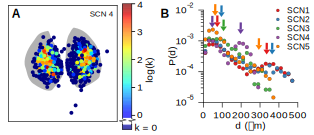
\includegraphics[width=3.5in]{chap3/figures/fig5_new.pdf}
    \end{center}
    \caption{\label{fig:dist}  Hubs of the small-world network are located in the central SCN. (\textbf{A}) Heatmap of node degree (color $\propto \log (k)$) distribution for a representative SCN shows that hubs of the small-world network are preferentially located in SCN core regions. All SCNs are shown in Figure \ref{fig:s6}.
    (\textbf{B}) Connection length ($d$ $\mu$m) distributions for SCNs 1-5 plotted on a semilog scale. Two peaks (arrows) are identifiable for SCNs 1,2,4,5: a ``local'' peak corresponding to connections between physically nearby neurons, and a second peak corresponding to the distance for functional connections between central SCN regions. For SCN3 these peaks are indistinguishable due to lack of spatial separation between cores.
}
\end{figure}


\begin{figure}[p]
    \begin{center}
        \includegraphics[width=6.5in]{chap3/figures/s6.pdf}
    \end{center}
    \caption{\label{fig:s6}
    Hubs of the small-world network are located in the central SCN. 
    (\textbf{A}) Inferred networks are shown overlaid on SCN tissue shape (gray). Connections between nodes are particularly dense in core regions and individual connections are difficult to distinguish. The 3rd ventricle is oriented at the top of each network. Strong functional connections between halves indicate that the core regions communicate to establish consistent phase to entrain the shell. Cells which have no or few functional connections are preferentially located in the outer SCN shell regions.
    (\textbf{B}) Heatmaps of node degree (color $\propto \log (k)$) distribution show that hubs of the small-world network are preferentially located in SCN core regions.
}
\end{figure}
}


Commonly, studies of the SCN have revealed two clusters of cells: a ventral core region defined by excitatory (phase attractive) GABAergic connections, VIP production, and light input from the retinohypothalamic tract \cite{Albus2005, Evans2013, DeWoskin2015, Welsh2010}.
To examine how this core-shell paradigm relates to the functional network, we examined the spatial hierarchy of the network.
Figure \ref{fig:dist}A illustrates the spatial hierarchy of node degree distribution across a representative SCN.
A lower node degree was observed in the shell region, relative to the higher node degree generally seen in the SCN core, obtained by our inference method. 
We note that in each SCN, a number (average 45\%) of cells in the SCN displayed no functional connections.
These cells are primarily located in the shell regions (Figure \ref{fig:dist}A).
This does not indicate that there are no physiological connections, since shell neurons do resynchronize with the rest of the SCN.
More likely, connections in this region are weaker and insufficient to rapidly resynchronize these cells above our functional connection MIC threshold.
This structure is consistent even when accounting for phase lags between individual cells within the fully synchronized SCN (see Figure \ref{fig:s4} following the main results).
Strikingly, this result of one cluster and the \textit{absence} of a second cluster differs from prior studies of the functional organization of the SCN, which identified two phase clusters of neurons \cite{Evans2013}.


The distribution of functional path distances ($d$) is shown in Figure \ref{fig:dist}B.
The functional path distance is defined as the physical separation between two functionally-connected cells.
This distribution also appears exponential for each network, where the likelihood of a connection existing at distance $d$ exponentially decays with this $d$.
These distributions are not strictly unimodal, rather, SCNs 1, 2, 4, and 5 display a second peak (identifiable via continuous wavelet transform peak detection) which corresponds to the physical separation between core regions.
SCN3 lacks this second peak as the identified cores of each half lack spatial separation.
The presence of this second peak indicates that core-core functional connections within a SCN are more prominent than average long-range functional connections.
Furthermore, it indicates that core-core coupling is tighter than core-shell coupling.


\subsection*{Relationship between physical and functional networks via network resimulation}

Since the physical connections between cells cannot be directly probed, we focused on obtaining the \textit{functional} network structure.
Here, we simulated the TTX experiment using stochastic circadian oscillator networks (using models from \cite{Gonze2006, Schroder2012, Abel2015a}) to determine how the functional network we infer is related to the underlying physical connectivity in the SCN.
First, we tested the efficacy of this method for inferring simulated physical networks of 400 cells with either linear nearest neighbor, small world Watts-Strogatz \cite{Watts1998}, or random network topology.
Next, we simulated the networks we inferred from SCN slices and show that our method can re-infer these physical networks with good accuracy.
Details regarding these simulations are included in the Supplement.

In Figure \ref{fig:s7}, we show representative traces from these simulations and further demonstrate that our method is able to recapture the underlying physical networks (random, Watts-Strogatz small-world, nearest neighbor) with accuracy dependent on the density of connections.
Functional networks inferred via our resynchronization and MIC method do not accurately recapture physical networks with dense random structure, as secondary indirect connections between nodes may be functionally identified as direct connections.
To validate the consistency of specific network structures inferred from TTX experiments, we simulated the SCN networks discovered in the previous section and again inferred the network from these simulations.
The resynchronization-MIC method performed well in recapturing simulated SCN networks, with an average area under the ROC curve (AUC) of $0.94$ for the three-state model and $0.80$ for the more complex eleven-state model.
The ROC curves are plotted for each SCN in Figure \ref{fig:s8}.
We note that the false positives are most often incurred in distinguishing between primary and secondary connections within dense regions, while disconnected nodes are easily identified.
Thus, this methodology can distinguish well between regions with dense and sparse physical connections such as the core and shell, but is less apt at identifying the individual physical connections in each region.
\begin{figure}[p]
    \begin{center}
        \includegraphics[width=6.5in]{chap3/figures/s7.pdf}
    \end{center}
    \caption{\label{fig:s7}
    Accuracy of the MIC inference method depends on both network topology and average node degree. 
    (\textbf{A}) and (\textbf{B}) show representative simulations capturing the TTX-mediated resynchronization for the three-state and eleven-state models, respectively.
    Next, MIC network inference was performed for simulated networks of three topologies: (\textbf{C}) random, (\textbf{D}), linear nearest neighbor, and (\textbf{E}) Watts-Strogatz small world ($\beta=0.05$).
    These networks are only shown for visualization of network structure.
    Simulated networks each contained 400 cells to match SCN recordings, and the average AUC was calculated for 5 dynamically-generated networks of each node degree.
    The area under the ROC curve is plotted as a function of average node degree for the three-state circadian model \cite{Gonze2006,Schroder2012} (\textbf{D}) and the eleven-state circadian model \cite{Abel2015a} (\textbf{E}) for these network structures.
    We show that both node degree and network structure affect the accuracy of this method.
    In general, networks that have a shorter average path length and higher average node degree are more difficult to accurately infer, as it becomes increasingly difficult to differentiate between direct and indirect physical connections.
}
\end{figure}

\begin{figure}[p]
    \begin{center}
        \includegraphics[width=6.5in]{chap3/figures/s8.pdf}
    \end{center}
    \caption{\label{fig:s8} Receiver operating characteristic (ROC) curve ranges and mean AUC values for simulation and inference of the SCN networks with physical connections dictated by the functional network, using (\textbf{A}) the three-state \cite{Gonze2006,Schroder2012} and (\textbf{B}) the eleven-state \cite{Abel2015a} models. Shaded ranges were calculated from 7 simulations using unique random seeds. We note that all neurons are simulated, including those which are unconnected. Unconnected neurons do synchronize experimentally though at a slower rate. To reflect this, unconnected cells in simulation were connected to the mean field, but at a reduced coupling strength. Errors in this method are largely incurred by secondary connections within tightly coupled regions (i.e. physical connections of cell 1 $\rightarrow$ cell 2 $\rightarrow$ cell 3 often show the additional cell 1 $\rightarrow$ cell 3 functional connection). Thus, we may understand that errors are incurred by functional connections in regions of dense physical connectivity appearing more dense.
}
\end{figure}




\begin{figure}[p]
    \caption{\label{fig:s4}
Effect of phase offset on MIC network inference.
    MIC is not phase-agnostic, and so the question arises of whether the inferred functional networks are driven by phase distributions in each SCN, similar to the phase clusters identified in \cite{Evans2013}.
First, we show how phase offset affects MIC score for pairs of synchronized oscillators.
Next, we show that re-aligning out of phase trajectories and taking the maximum MIC reduces much of this bias.
Finally, we examine how this affects the connections we identify in the five SCN tissues, and show that our results are consistent after applying this phase offset correction.
    (\textbf{A})
    The MIC score varies with phase offset between two phase-locked oscillators.
    Each point on this plot was generated by simulating 50 pairs of strongly coupled cells, as in S2.
    Connected cells in this model synchronize to a phase offset of 0h because they are parameterized identically.
    One trajectory from each pair was phase-shifted in 0.1h increments up to 12h, to generate a range of phase offsets between the trajectories.
    The mean MIC score (y-axis) of the 50 pairs was then computed for each artificially-created phase offset (x-axis).
    As the phase offset between coupled cells is increased, the MIC score is reduced from its maximum at a 0h angle.
    This is considered the uncorrected case, where MIC is computed with no regard for the phase offset between trajectories.
    (\textbf{B})
    Next, we took the phase-shifted trajectories from (A) and performed a correction to renormalize MIC, so that MIC score is not affected by the phase offset between cells which we originally added.
    The correction was performed by again shifting the trajectories 12h in either direction, this time in intervals of 1.0h to reflect experimental sampling rate, and calculating MIC scores at each of these shifts.
    We then selected the largest of the resulting values as the MIC score for the cell pair, as this maximum MIC corresponds to when phases are realigned.
    In comparison to the uncorrected method, the maximum MIC correction results in reduced sensitivity to the phase offset between cells, as the corrected MIC score (y-axis) is nearly flat with respect to the phase offset of the pair (x-axis).
    This method reduces power however, as some of the initial resynchronization period must be truncated in order to realign phases, resulting in a slight bias toward \textit{larger} phase offsets.
    Thus, the uncorrected method (biased toward small phase offset) and corrected maximum MIC method (slightly biased toward large phase offset) form bounds on connectivity.
    (\textbf{C}) Scatter plot of MIC score vs. mean phase offset for all possible connections within each SCN.
    There is a clear bias against absolute phase offsets greater than $\sim2$h (left), in a similar form to (A).
    This bias is rectified by performing the maximum MIC correction (right).
    Phase offset (used only for plotting purposes) was calculated by a Hilbert transform after removing the trend via discrete wavelet baseline detrending.
    As the phase offset was unstable early during resynchronization, it was calculated after it had stabilized, during days 6-7.
}
\end{figure}

\begin{figure}[p]
\contcaption{(Continued.)
        (\textbf{D}) Plot of standard deviation of phase offset vs. mean phase offset for possible and identified connections within all five SCNs.
    Standard deviation of phase offset was calculated throughout the resynchronization period, and can be thought of as a measure of phase offset instability between two cells.
    As expected, MIC detects connections between cells with a low standard deviation in phase offset for both cases, with a wider range of mean phase offsets .
    Thresholds were raised for each of the five SCNs (to 0.980, 0.970, 0.999, 0.985, 0.985 respectively) after phase correction, as all MIC scores are increased by this method.
    Generally, cell pairs with a larger phase offset also had a less stable phase offset, such that even after phase offset correction most connections were between cells with an difference in phase of less than 2h.
    (\textbf{E}) Phase-corrected SCN networks maintained small-world characteristics, with a comparable mean path length and larger clustering coefficient than corresponding random networks.
(\textbf{F}) Node degree distributions for each SCN remain exponential (P<0.0001 for each SCN, likelihood-ratio test comparison with power law fits), though $\lambda$ changes corresponding to the increased average node degree for SCNs in which phases were aligned.
    SCN 3 deviates slightly from the others here, due to the high number of connections which yield saturated (1.0) MIC scores after re-alignment.
    (\textbf{G}) Connection length distributions for unaligned and phase-aligned networks. 
    Despite the higher average node degree for aligned networks, these distributions continued to display two peaks: one for local connections within a core, and a second corresponding to core-core connections.
(\textbf{H}) Similarly, core-shell hierarchy was maintained after phase-alignment. Additionally, many shell neurons remain functionally ``unconnected,'' indicating a much slower resynchronization than neurons in SCN core regions.
    These neurons do synchronize, however, they are less tightly synchronized than cells which have identifiable connections.}
\end{figure}

\begin{figure}[p]
    \begin{center}
        \includegraphics[width=4.15in]{chap3/figures/s4_new.pdf}
    \end{center}
\contcaption{(Continued.)}
\end{figure}

\section{Discussion}

In this work, we inferred the functional network of the suprachiasmatic nucleus during resynchronization through the use of a TTX-mediated resynchronization and the maximal information coefficient.
The functional networks we found were consistent across all samples, displaying small-world characteristics, a discrete exponential node degree distribution, and core-shell spatial hierarchy in which densely functionally-connected cores synchronize rapidly.
Our results are consistent with previous studies which show differences in function and neurotransmitter activity between core and shell SCN neurons \cite{Albus2005, Yan2005, Evans2011, Evans2013, Watanabe2007, Welsh2010, Evans2015, Myung2015, DeWoskin2015}.
However, in this work for the first time we probe connectivity within these clusters.
This leads to two surprising results: a lack of a second functionally connected cluster in the shell region, and dense connections between SCN cores.

It is well-established that exposure to artificial long day or light:dark:light:dark frequency doubling conditions can split the SCN into core and shell phase clusters, which oscillate with a large phase lag and also result in behavioral splitting \cite{Watanabe2007,Evans2011,Evans2013}.
Although shell neurons form a phase cluster under these conditions, we found few functional connections within this region even when accounting for phase alignment, suggesting that the phase clustering is driven by a common response to light reception and mediated by the core SCN rather than driven by tight connectivity within the shell itself.
This is one particular advantage of the TTX assay we employ: light-based approaches are unable to differentiate between cells which have identical responses to a common stimulus, and cells which communicate to establish similar behavior.
A previous study of SCN reentrainment to shifted light exposure also showed that the ventral SCN reentrained rapidly, while the dorsal region took several days to reentrain \cite{Albus2005}.
It was proposed that the core entrained rapidly due to its receiving input from the retinohypothalamic tract (RHT), and showed that synchronization of the shell was mediated by the effect of excitatory GABA.
As our resynchronization conditions are chemically-induced and do not involve light input, it was unexpected that a fast-resynchronizing core/slow-resynchronizing shell is a conserved feature between these studies.
This consistency indicates that the underlying structure of the SCN, rather than simply RHT connection, drives the dominant role of the core SCN.

We did not attempt to identify connection directionality or the molecular mechanisms driving connectivity, and it is possible that multiple pathways are involved.
It has been shown that excitatory GABA action drives reentrainment of the shell region in response to light phase shifts \cite{Albus2005}.
This was examined in depth in recent collaborative works \cite{Myung2015, DeWoskin2015}; these studies demonstrated the encoding of day length through the GABA pathway, by the Cl$^-$-dependent excitatory (core, phase-attractive) or inhibitory (shell, phase-repulsive) effects of slow-scale (tonic) GABA.
Visually, the core regions identified in our networks overlap with the regions of excitatory GABA action \cite{Myung2015}.
In future studies, our TTX-based assay could be combined with VIP/GABA/glutamate agonist or antagonist application and repeated in order to identify the molecular mechanisms responsible for the identified connections.
If GABA coupling affects differentiation between core hub neurons and shell neurons, this would result in significant seasonal plasticity of the functional network.

The functional networks we inferred contained a surprising number of connections between core regions of each suprachiasmatic nucleus.
The SCN is often thought to be most tightly connected within each half, given the ability of the left and right SCN to oscillate in antiphase in animals exposed to constant light \cite{Delaiglesia2000, Ohta2005}.
However, tight bilateral coupling is reflective of previous studies which showed significant coupling between the halves and further implicates the glutamate receptor in this communication \cite{Michel2013}.
This is especially interesting, since the glutamate receptor has also been implicated in communication between the SCN and the RHT, which occurs in the core SCN region \cite{Ebling1996}.
Thus, our results support the hypothesis that antiphasic oscillation between SCN halves in constant light is made possible by distinct signalling mechanisms in the SCN rather than a weaker coupling strength between halves \cite{Indic2008, Michel2013}.
It is unclear if connections between halves are synaptic or diffusive.

Theoretical studies in network science as well as modeling studies specific to the circadian field have pointed to possible advantages and causes of a small-world network structure.
Small-world exponential networks provide advantages in robustness due to having ``hubs'' of high node degree and many less-important nodes of low node degree.
Networks with this topology are better able to maintain short paths of communication when randomly-selected nodes are removed \cite{Albert2002}, due to the redundancy and long-range connections provided by network hubs.
This could occur during aging, as it is known that some brain regions lose mass during the aging process.
Small-world topology has also been shown to enhance synchronization and amplitude properties of the SCN with a lower energy cost (fewer connections) when compared to random and nearest-neighbor networks \cite{Vasalou2009, Hafner2012}.
Theoretical studies have predicted that spatially embedded small-world networks, such as neuronal networks, would display an exponential node degree distribution as seen in our data \cite{Ozik2004, Zitin2014}.
This distribution would result from growth of a small initial population of connected nodes.
As more nodes are added, the neuron population is forced to move spatially and initial local connections ultimately become long-range, while new short-range connections form.
In this context, it is striking to note that the fetal SCN forms as neurons are added to the core first and then shell regions. The connections we measure, therefore may reflect the ontogeny of synapse formation in the SCN. 
If, however, core-core long range connections are found to be diffusive rather than synaptic, this hypothesis would not apply.
Future experiments could test whether the left and right SCN must form synapses to synchronize, for example, in co-cultures.

Our work presents both a new perspective on connectivity within the SCN and a new assay for observing communication between individual circadian neurons at high spatial resolution.
A major difficulty in mapping the SCN and the brain as a whole lies partly in the multiple time and physical scales at play.
One method alone is insufficient to map the whole SCN at all resolutions, necessitating multiple perspectives to achieve spatial, directional, and mechanistic specificity.
In conjunction with light-driven desynchronization assays, antagonist/agonist application, genetic knockdowns, and mathematical modeling, this TTX assay with correlation metrics can be used to further probe connections within the SCN at a single-cell level, and between the SCN and other brain regions.

Finally, although we have presented results indicating heterogeneous network structure within the SCN, we have not proposed a means by which this structure arsises.
Studies of the onset of circadian oscillation in the fetal SCN have been limited to whole-SCN analyses, in part due to the experimental challenge of explanting the fetal SCN and recording the activity of distinct neurons.
In the ensuing chapter, we begin to approach questions of ontogeny of cell-autonomous circadian rhythms in SCN neurons, and how and when the network driving circadian synchrony arises.
Importantly, the core-shell heterogeneity of the SCN observed in this study as well as others provides a marker for a ``mature'' SCN network.




























\chapter{Ontogeny of circadian rhythms and synchrony in the suprachiasmatic nucleus}
\blfootnote{Major portions of this chapter appear as V.~Carmona-Alcocer, J.H.~Abel, T.C.~Sun, L.R.~Petzold, F.J.~Doyle~III, C.L.~Simms, and E.D. Herzog, ``Ontogeny of circadian rhythms and synchrony in the suprachiasmatic nucleus,'' Journal of Neuroscience, accepted. All statistical and mathematical analysis and modeling was performed by J.H. Abel. All experimental work was performed by members of the Herzog lab, primarily V.~Carmona-Alcocer. This journal article, and thus a major portion of this chapter, was written collaboratively with V.~Carmona-Alcocer and E.D. Herzog.
%copyright info email sent: http://www.jneurosci.org/sites/default/files/files/permissions_policy.pdf
}

\section{Introduction}
How and when hypothalamic circadian rhythms arise during development is not known.
More precisely, it has not been established when cell-autonomous circadian rhtyhms in the SCN arise, and how and when the network establishing intercellular synchrony first appears.
Studies of whole-SCN circadian development do not make the distinction between single-cell and whole-tissue oscillation, further obscuring the development of the SCN network, which is necessary for synchronous oscillation.

In mice, it is well-established that neurogenesis of the SCN occurs between embryonic days 10-15 (termed E10-15, where E1 is the day when a vaginal plug is detectable), peaking between E12-14 and forming from ventrolateral to dorsomedial \cite{Shimada1973,  Kabrita2008, Shimogori2010}.
It is further known that a variety of transcription factors are expressed during differentiation of the SCN (e.g.\ \textit{Lhx1}, \textit{Shh}, \textit{Six3}, \textit{Six6}) \cite{Shimogori2010, VanDunk2011, Clark2013, Bedont2014}.
Development also continues postnatally, and synaptogenesis has been found to occur primarily after birth \cite{Moore1989, Shimogori2010}.
Although the SCN continues to develop after birth, numerous studies in rats have shown that circadian rhythms in fetal metabolism, and circadian spontaneous electrical activity and clock gene expression within fetal SCN, begin before birth \cite{reppert1983maternal, reppert1984suprachiasmatic, Shibata1987, Sladek2004, Kovacikova2006, Houdek2014}.
Studies of mice have yielded similar results to rat studies, with detectable fetal daily rhythms in \textit{Per1} transcript levels at E17, and PER1 and PER2 proteins by E18 \textit{in vivo} \cite{Shimomura2001, Ansari2009}.
\textit{In vitro} studies of SCN explants have found circadian expression of the PERIOD2::LUCIFERASE (\textit{Per2}$^{Luc}$) bioluminescent reporter in the whole SCN as early as E13 \cite{Landgraf2015} or E15 \cite{Wreschnig2014}.
Still, it remains unclear if these oscillations are self-sustaining and spontaneously synchronizing as in the mature SCN, or driven or coordinated by the circadian oscillator of the mother.

In the mature SCN, neurons exchange electrical and neurotransmitter signals to maintain identical periods and consistent phase relationships \cite{Mohawk2011, Herzog2015, Evans2016}. 
Among these signals, vasoactive intestinal peptide (VIP) has attracted significant attention for its essential role in SCN synchrony \cite{Aton2005}.
The absence of VIP or its receptor, VIPR2, reduces synchrony between neurons and consequently eliminates many daily rhythms, while exogenous application of VIP is able to restore synchrony to the VIP$^{-/-}$ SCN \textit{in vitro} \cite{Harmar2002, Colwell2003, Aton2005, Maywood2006, Ciarleglio2009}.
It remains unknown when VIP is first expressed in the SCN, and whether its role in the fetal SCN is identical to that in the adult \cite{Wang2014, Ono2016}.
For example, GABA, another neurotransmitter expressed in the SCN, is known to have very different effects in the fetal brain because of differing chloride potentials \cite{fain1999}.
In this chapter, we used the \textit{Per2}$^{Luc}$ bioluminescent reporter to study the onset of circadian rhythms in the SCN at at near-single-cell scale.
We sought to identify the onset of self-sustained genetic circadian oscillations in individual cells, spontaneous synchronization within the explanted SCN, and other markers of the mature SCN including expression of neurotransmitters with circadian relevance.

\section{Materials and methods}

\subsection*{Animals}
All mice were maintained on a C57BL/6JN background (WT) and housed in a 7am-7pm light-dark cycle in the Danforth Animal Facility at Washington University.
The $Per2^{Luc}$ mouse line was generated by replacing the endogenous mouse \textit{Period2} gene locus with a $Per2^{Luc}$ reporter construct \cite{Yoo2004}.
For immunochemistry, we compared male and female homozygous $Per2^{Luc}$ pups to $Vip^{-/-}$ and $Vipr2^{-/-}$ pups as negative controls.
Vaginal plugs confirmed overnight mating of each female.
We designated the morning after mating as embryonic day 0.5 (E0.5) and the day of birth as postnatal age 0 (P0).
All procedures were approved by the Animal Care and Use Committee of Washington University and followed National Institutes of Health guidelines.

\subsection*{Cultures and bioluminescence recording}
Pregnant mice were euthanized with CO$_2$ and cervical dislocation and their embryos dissected into 4$^\circ$C Hanks Buffered Saline Solution (Sigma).
All surgeries started at 1:00 PM (Zeitgeber Time, ZT 06).
We recorded bioluminescence from 300 $\mu$m coronal SCN slices from fetal (E13.5-E15.5 and E17.5) and postnatal (P2) homozygous $Per2^{Luc}$ mice \cite{Landgraf2015}.
Briefly, brains were embedded in a block of 4\% low-melting agarose and prepared with a vibraslicer.
SCN were dissected with scalpels from sections of the ventral hypothalamus and placed on 0.4 mm membrane inserts (Millipore) in sealed 35 mm Petri dishes (BD Biosciences) with 1 mL Dulbecco's Modified Eagle Medium (Sigma, pH 7.2), supplemented with 25 U/mL penicillin, 25 $\mu$g/mL streptomycin (Invitrogen), 10 mM HEPES (Sigma), 2\% B27 (Invitrogen), 0.35 g/L NaHCO3 (Sigma) and 0.15 mM beetle luciferin (Promega).
SCN explants were transferred to a light-tight incubator at 36$^\circ$C (Onyx, Stanford Photonics).
We collected images (XR Mega-10AW camera, Stanford Photonics) every 6 min (6 sec exposure) and then summed every 10 frames with ImageJ software (http://rsbweb.nih.gov/ij) to provide one image every hour.
We applied adjacent frame minimization to each movie to filter out bright noise caused by the camera or cosmic rays.

\subsection*{Data analysis}
We analyzed the $Per2^{Luc}$ rhythms of the developing SCN at the level of the whole tissue and with 30 $\mu$m (pixel) resolution.
The statistical analysis for each experiment is described in detail in its respective section.
We assessed rhythms measured as the integrated intensity of the SCN tissue with cosinor analysis (software from B. Meier and A. Kramer).
We performed a pixel-based analysis of the same SCN movies.
We excluded movies if the corners of the SCN slice moved (3 slices excluded at each of E15.5, 17.5 and P2).
We measured periodicity of each pixel (1 px = 900 $\mu$m$^2$) and defined pixels as circadian if they had a dominant period between 18-32h with $P < 0.05$ by Lomb-Scargle periodogram analysis \cite{Ruf1999}; or a correlation coefficient greater than 0.6 in cosinor analysis.
Because the two methods yielded 90 $\pm$ 0.02\% (mean $\pm$ S.E.; n=30 brains) agreement in pixel classification, we reported results from the periodogram analysis only.
The cycle-to-cycle variability in $Per2^{Luc}$ was evaluated by detrending rhythmic cells with a discrete wavelet transform \cite{Leise2011} keeping only detail coefficients between 16-32h, and measuring the interpeak distance (h) of each cycle.
We evaluated the synchrony index using the Kuramato method \cite{kuramoto1984}, with instantaneous phase calculated using a Hilbert transform of the detrended and denoised data.

A radial distribution of mean peak times was constructed for each SCN to identify the presence of core-shell structure.
The time of the initial peak for each pixel was calculated following detrending.
A radial distribution of peak times was constructed by binning individual cell peaks based on radial distance from a reference point in the left ventrolateral SCN.
A null distribution of radial peak times was calculated by bootstrapping: reassigning peak time values at random to pixels within each SCN and recalculating the radial distribution using 10,000 bootstrap runs.
An SCN was determined to have core-shell structure if the radial peak time distribution showed significant (P < 0.05) peaks for the shell region (early-peaking, middle distances) and at least one core region (late-peaking, near and far distances). 

\subsection*{Software}
Data analysis was performed in the Python language, using packages scipy and numpy \cite{jones2014scipy}, PyWavelets, Statsmodels \cite{Seabold2010}, and Matplotlib \cite{Hunter2007}.
Parallelization of data processing was achieved via iPython \cite{Perez2007}.

\subsection*{Immunocytochemistry}
Brains of mice from ages E13.5-E17.5, P0 and P2 were removed and fixed in 4\% paraformaldehyde in phosphate buffered saline (PBS) overnight at 4$^\circ$C.
We transferred them to 30\% sucrose in PBS for 24 h at 4$^\circ$C and sectioned in 30 $\mu$m thick coronal slices onto microscope slides.
The sections were incubated for 1 h at 4$^\circ$C in a blocking solution (10\% not fat dry milk, 10\% bovine serum albumin and 0.3\% TritonX-100 in PBS) and then for 48 h at 4$^\circ$C in an anti-VIP (1:1000, Imunostar) or anti-VPAC2R (1:1000, Abcam) rabbit polyclonal antibody diluted in 3\% BSA and 0.35\% TritonX-100 in PBS.
After washing in PBS, the slides next were incubated at room temperature in a biotinylated goat anti-rabbit IgG (1:200; Vector) for 2 h and then ABC solution (1:200; Vectastain Elite ABC Kit, Vector) for 2 h.
Finally, we incubated each slide in 50 mM Tris-HCl using 3,3-diaminobenzidine kit (Sigma).
After each step, we rinsed 3 times for 15 minutes in PBS.
Mounted sections were dehydrated through a series of ethanol and xylene washes.
Slides were imaged (NanoZoomer microscope, Leica) and the integrated optical density of the SCN was measured using ImageJ software \cite{Schneider2012}.

\subsection*{Drug treatments} 
All drugs were diluted in deionized water and they remained in the recording medium throughout the entire recording without further medium changes.
VIP antagonist (200nM PG-99465) provided by Dr.\ P.\ Robberecht \cite{Cutler2003}, GABA antagonist (100 $\mu$M Gabazine, TROCRIS), MEC (10 $\mu$M Meclofenamic acid, SIGMA), or TTX (2.5 $\mu$M tetrodotoxin).


\section{Results}

\subsection*{SCN cells become reliable circadian oscillators after E14.5}
\begin{figure}[p]
    \begin{center}
        \includegraphics[width=3.3in]{chap4/figures/Figure1.png}
    \end{center}
    \caption{\label{fig:vc1} {\small Circadian rhythms in the SCN during development.  Long-term, real-time recordings of PER2 expression from SCN harvested after E14.5 showed reliable circadian periods between 18-32h. (\textbf{A}) Representative records of $Per2^{Luc}$ bioluminescence from SCN starting on the day they were explanted. Note the weak circadian oscillations that were found in some E14.5 SCN. Insets show images of two representative SCN from each age. Some SCN harvested at E13.5 expressed $Per2^{Luc}$ above the SCN region along the ventricular zone of dorsal hypothalamus (blue arrow head, n=5/8). All others harvested at this age and older reliably expressed high levels of PER2 in the bilateral SCN. Scale bar = 10 px = 300 $\mu$m. (\textbf{B}) Nearly all SCN expressed significant circadian rhythms when harvested on or after E15.5 (Upper panel), with periods close to 24 h (mean ± SEM; Middle panel) and durations of daily $Per2^{Luc}$ expression above the mean close to 12 h (alpha; mean $\pm$ SEM, Lower panel; *P < 0.05, one-way ANOVA, Tukey's HSD). Note, 8 slices were examined at E13.5, however, we excluded 5 because they did not express detectable PER2 in the SCN region.}
    }
\end{figure}

Recent in vitro studies have demonstrated the presence of circadian rhythms in PER2 expression in whole SCN explants at E13 \cite{Landgraf2015} or E15 \cite{Wreschnig2014}, around the times of peak or completed neurogenesis, respectively.
To test if cell-autonomous oscillations appear prior to tissue-level rhythms, we imaged bioluminescence in fetal $Per2^{Luc}$/$Per2^{Luc}$ SCN slices.
SCN explanted at E13.5 displayed no tissue-level circadian rhythms (n = 8 SCN from 2 litters; Fig. 
\ref{fig:vc1}).
At this stage, the ventricular zone of dorsal hypothalamus expressed high levels of PER2, sometimes in a circadian pattern (n = 2 of the 8 slices), but the bilateral SCN region had low to no PER2 expression and no circadian rhythms.
In contrast, all tissues explanted on E14.5 or later displayed bilateral $Per2^{Luc}$ expression in the ventral hypothalamus, corresponding to the SCN.
By E14.5, 45\% of SCN were circadian (5 of 11 SCN from 4 litters).
Notably, some E14.5 explants (n = 4 of 11) also displayed no rhythmic $Per2^{Luc}$ expression outside the SCN in the ventricular zone of the dorsal hypothalamus.
By E15.5, no hypothalamic explants showed high PER2 expression outside the SCN region and nearly all SCN were circadian (n = 11 of 12 E15 SCN from 4 litters, 7 of 7 E17 SCN from 2 litters and 5 of 6 P2 SCN from 1 litter).
We conclude that PER2 expression is localized to the SCN and becomes circadian on E14.5.

\begin{figure}[p]
    \begin{center}
        \includegraphics[width=6.5in]{chap4/figures/Figure2abcd_vc.png}
    \end{center}
    \caption{\label{fig:vc2} Embryonic SCN cells express PER2 rhythmically beginning around E14.5 in vitro. (\textbf{A}) Heat maps of two SCN explanted at each developmental stage show circadian pixels based on Lomb-Scargle periodogram (power above P < 0.05) and Cosinor analysis (correlation coefficient greater than 0.6). We therefore report results only from periodogram analyses for simplicity. (\textbf{B}) Representative Per2Luc bioluminescence images of the same SCN explants (1 h integration, 2 x 2 binning). Scale bar = 10 px = 300 $µ$m. (\textbf{C}) Representative Per2Luc bioluminescence recordings from single rhythmic pixels from SCN cultured at different embryonic stages. Note the competence of the E15.5 SCN to generate and sustain circadian rhythms in PER2 protein expression. (\textbf{D}) The fraction of circadian pixels in each SCN (mean $\pm$ SEM,) was higher for explants at E15.5 and older (*P < 0.05, one-way ANOVA, Tukey's Honestly Significant Difference (HSD), n=at least 3 SCN at each age where age is reported as days post mating, E0.5, and post birth, E20.5=P0). 
    }
\end{figure}


We next developed methods to culture and image the embryonic SCN for at least 5 days.
From these movies, we quantified local circadian rhythms where each pixel included approximately 10 or fewer cells (Fig. 
\ref{fig:vc2}A-B).
We found the fraction of circadian pixels (cells) increased approximately 7-fold from E14.5 (Fig. 
\ref{fig:vc2}C-D; 0.10 $\pm$ 0.07, mean $\pm$ SEM; n=11 SCN from 4 litters) to E15.5 (0.72 $\pm$ 0.11; n = 9 SCN from 4 litters; *P < 0.05, one-way Kruskal-Wallis H(3)=10.62, with posthoc Tukey's Honestly Significant Difference).
Nearly all regions were circadian in SCN explanted on E17.5 (0.96 $\pm$ 0.03; n = 4 SCN from 2 litters) and postnatal day 2 (P2, 0.97 $\pm$ 0.02; n = 3 SCN from 1 litter).  
The developmental increase in the number of circadian regions correlated with an increase in circadian period in the SCN (Fig. 
\ref{fig:vc3}A-B).
We conclude that a small number of SCN cells initiate endogenous circadian rhythmicity by E14.5, and by E15.5 SCN cells are rhythmic throughout the SCN.

To determine the precision of SCN rhythms during development, we measured the cycle-to-cycle difference in period for each pixel within the fetal SCN over three days of the recording. Interestingly the increase in the number of circadian oscillators correlated with an increase in circadian precision (Fig. 
\ref{fig:vc3}C-D), suggesting that addition of circadian cells lengthens and stabilizes period in the SCN.

\begin{figure}[p]
    \begin{center}
        \includegraphics[width=6.5in]{chap4/figures/Figure3_vc.png}
    \end{center}
    \caption{\label{fig:vc3} Circadian period and precision of SCN cells increased with development. (\textbf{A}) Heat maps from representative SCN show the mean period over 5 days of recording. (\textbf{B}) The fraction of rhythmic pixels correlated with an increase in the mean SCN period (Least-squares linear regression P = 0.00019, Pearson's r = 0.74. SCN with fewer than 5 circadian pixels were considered arrhythmic and excluded from this analysis.  E14.5: diamonds, n=6 of 11, E15.5: circles, n=9 of 9, E17.5: triangles, n=4 of 4, P2: squares, n=3 of 3).  (\textbf{C}) Representative mean cycle-to-cycle variability heat maps show the increase in circadian precision with age. Scale bar = 150 $\mu$m. (\textbf{D}) The average variability of the daily period across all rhythmic pixels within each isolated SCN inversely correlated with the fraction of circadian cells (least-squares linear regression P = 0.0006, Pearson's r = -0.70; symbols as in B), SCN with fewer than 5 circadian pixels were considered arrhythmic and excluded from this analysis.
    }
\end{figure}

\begin{figure}[p]
    \begin{center}
        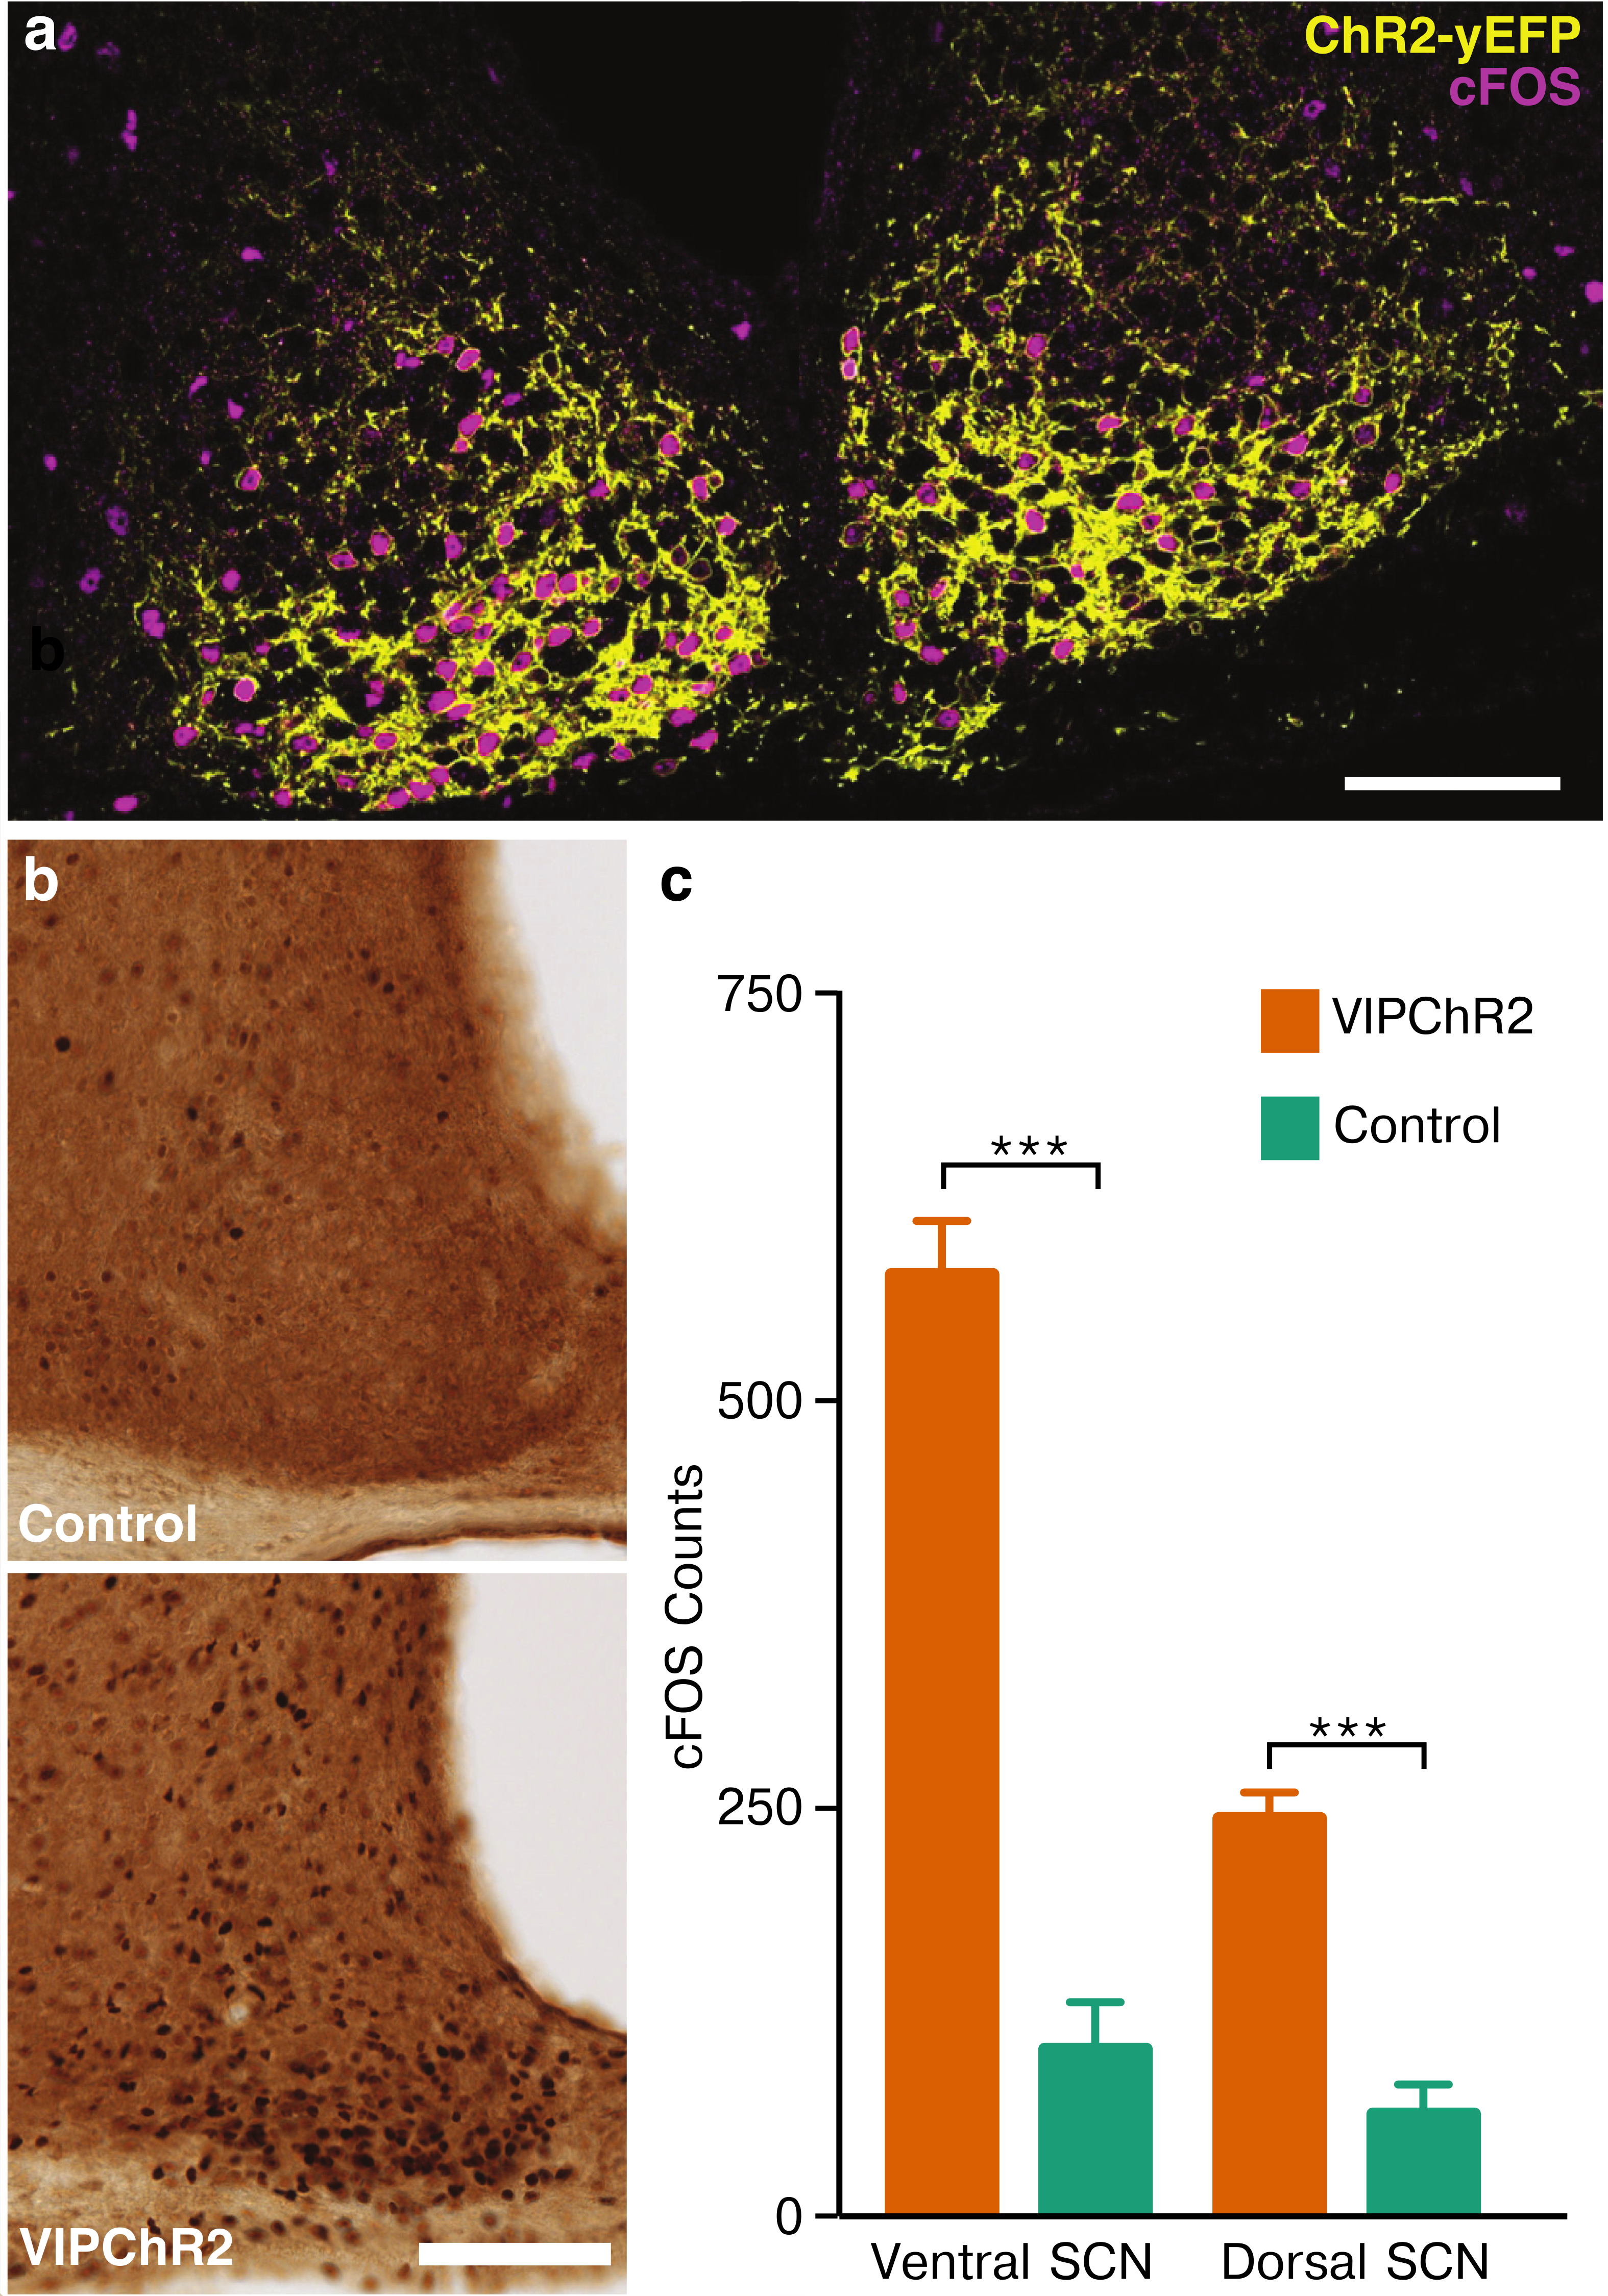
\includegraphics[width=3.5in]{chap4/figures/Figure4.png}
    \end{center}
    \caption{\label{fig:vc4} The phase wave of PER2 expression in the SCN appeared only after birth. (\textbf{A}) Heat maps of the time of peak PER2 expression across representative SCN. Note the dorsal-to-ventral distribution across the cells of the P2 SCN. Scale bar = 300 $\mu$m. (\textbf{B}) Radial distribution of peak times revealed a core-shell structure in the P2, but not younger, SCN explants. We compared the average differences in the times of peak PER2 expression as a function of distance from the ventral margin of each SCN with a null distribution of randomly shuffled peak times (shaded area=95\% CI for mean peak time calculated from 10,000 resamples). At P2, PER2 peaked significantly later in the ventral core than the dorsal shell, as seen in this representative example. 
    }
\end{figure}


\subsection*{The phase wave typical of adult SCN appears around P2}


In adults, PER2 expression progresses as a daily wave from dorsal to ventral across the SCN \cite{Yan2002, Quintero2003, Yamaguchi2003, Evans2011}.
We examined when this spatiotemporal patterning of circadian expression arises in the SCN. To do so, we identified the times of daily peak PER2 in each pixel of the SCN and tested for spatial organization of expression.
We found reliable daily waves of PER2 from the dorsal to ventral SCN by P2, but not at earlier developmental stages (Fig. 
\ref{fig:vc4}).
We conclude that phase relationships among SCN cells continue to mature after birth.



\subsection*{Onset of synchrony and intercellular communication within the SCN}

Synchronous circadian oscillations in the SCN are required to coordinate daily rhythms in behavior \cite{Schwartz1987, Aton2005, Ohta2005}.
To test how synchrony develops, we measured the cycle-to-cycle variability in period length and the synchrony index (SI), a quantity that ranges from 1.0 (all oscillators peak together) to 0.0 (all cells peak at uniformly different times of day) from five days of recording.
We found that synchrony tends to increase between E14.5 (Fig. 
\ref{fig:vc5}; SI = 0.80$\pm$0.5, n = 6 SCN) and E15.5 (SI = 0.87$\pm$0.05, n = 9 SCN) reaching a maximum around E17.5 (SI = 0.91$\pm$0.02, n = 4) and P2 (SI = 0.94$\pm$0.02, n = 3 SCN (one unilateral due to changes during recording between halves)). 
Although there is no significant differences in the SI between ages, SI was positively correlated with the fraction of SCN cells displaying daily rhythms, indicating that intercellular synchrony is developed simultaneously with increased endogenously generated cellular oscillation (Fig. 
\ref{fig:vc5}C). 



We next examined the signaling pathways that could enable synchronization of SCN cells starting around E15.5.
VIP signaling is necessary for coordinated circadian rhythms among SCN cells and in behavior of adult mice \cite{Harmar2002, Colwell2003, Aton2005, Maywood2006, Ciarleglio2009}.
We measured the levels of VIP, and its cognate receptor, VIPR2, by immunocytochemistry between days E14.5 and P2 (Fig. 
\ref{fig:vc6}).
We found VIP (12.5$\pm$2.3, n = 7) and VIPR2 (15.0$\pm$5.6 relative optical density (ROD), n = 6) were detectable postnatally above baseline (immunolabeling in the P2 SCN of $Vip^{-/-}$ = 2.1$\pm$0.7 ROD, n = 5 brains and $Vipr2^{-/-}$ =3.8$\pm$2.1 ROD, n = 5, mean$\pm$SEM), but not earlier stages.
To further explore this surprising result, we found that a VIP antagonist did not affect synchrony of the E15.5 SCN (Fig. 
\ref{fig:vc7}).
Consistent with prior publications, we found that addition of the VIPR2 antagonist reduced the fraction of circadian cells in the isolated adult SCN to 30\% from 84\% (n = 1 adult SCN; \cite{Cutler2003, Aton2005}.
We conclude that VIP and its receptor VIPR2 appear in the SCN after the initiation of circadian rhythms and are not required for circadian synchrony among embryonic SCN cells.

We then performed further pharmacological experiments to test if GABA and/or gap junctions, other candidate coupling mechanisms, might drive synchrony in the SCN before VIP expression begins. 
Remarkably, antagonists against either or both GABA and gap junctions did not reduce the synchrony index of the E15.5 SCN (Fig. \ref{fig:vc7}).


\begin{figure}[!p]
    \begin{center}
        \includegraphics[width=6.5in]{chap4/figures/Figure5.png}
    \end{center}
    \caption{\label{fig:vc5} The synchrony between SCN cells increased and became more stable as the fraction of circadian cells increased. (\textbf{A}) Representative traces of the synchronization index (also called the Kuramoto order parameter or Rayleigh Statistic, r) among regions within the cultured SCN at different ages. (\textbf{B}) The average synchronization index of SCN slices (mean $\pm$ SEM, 24 h excluded from either end of analysis) did not reliably increase with age, but (\textbf{C}) correlated with the fraction of circadian cells in the SCN (symbols as in prior figure, Least-squares linear regression P = 0.004, Pearson's r = 0.61, n=at least 3 SCN at each age).
    }
\end{figure}

\begin{figure}[!p]
    \begin{center}
        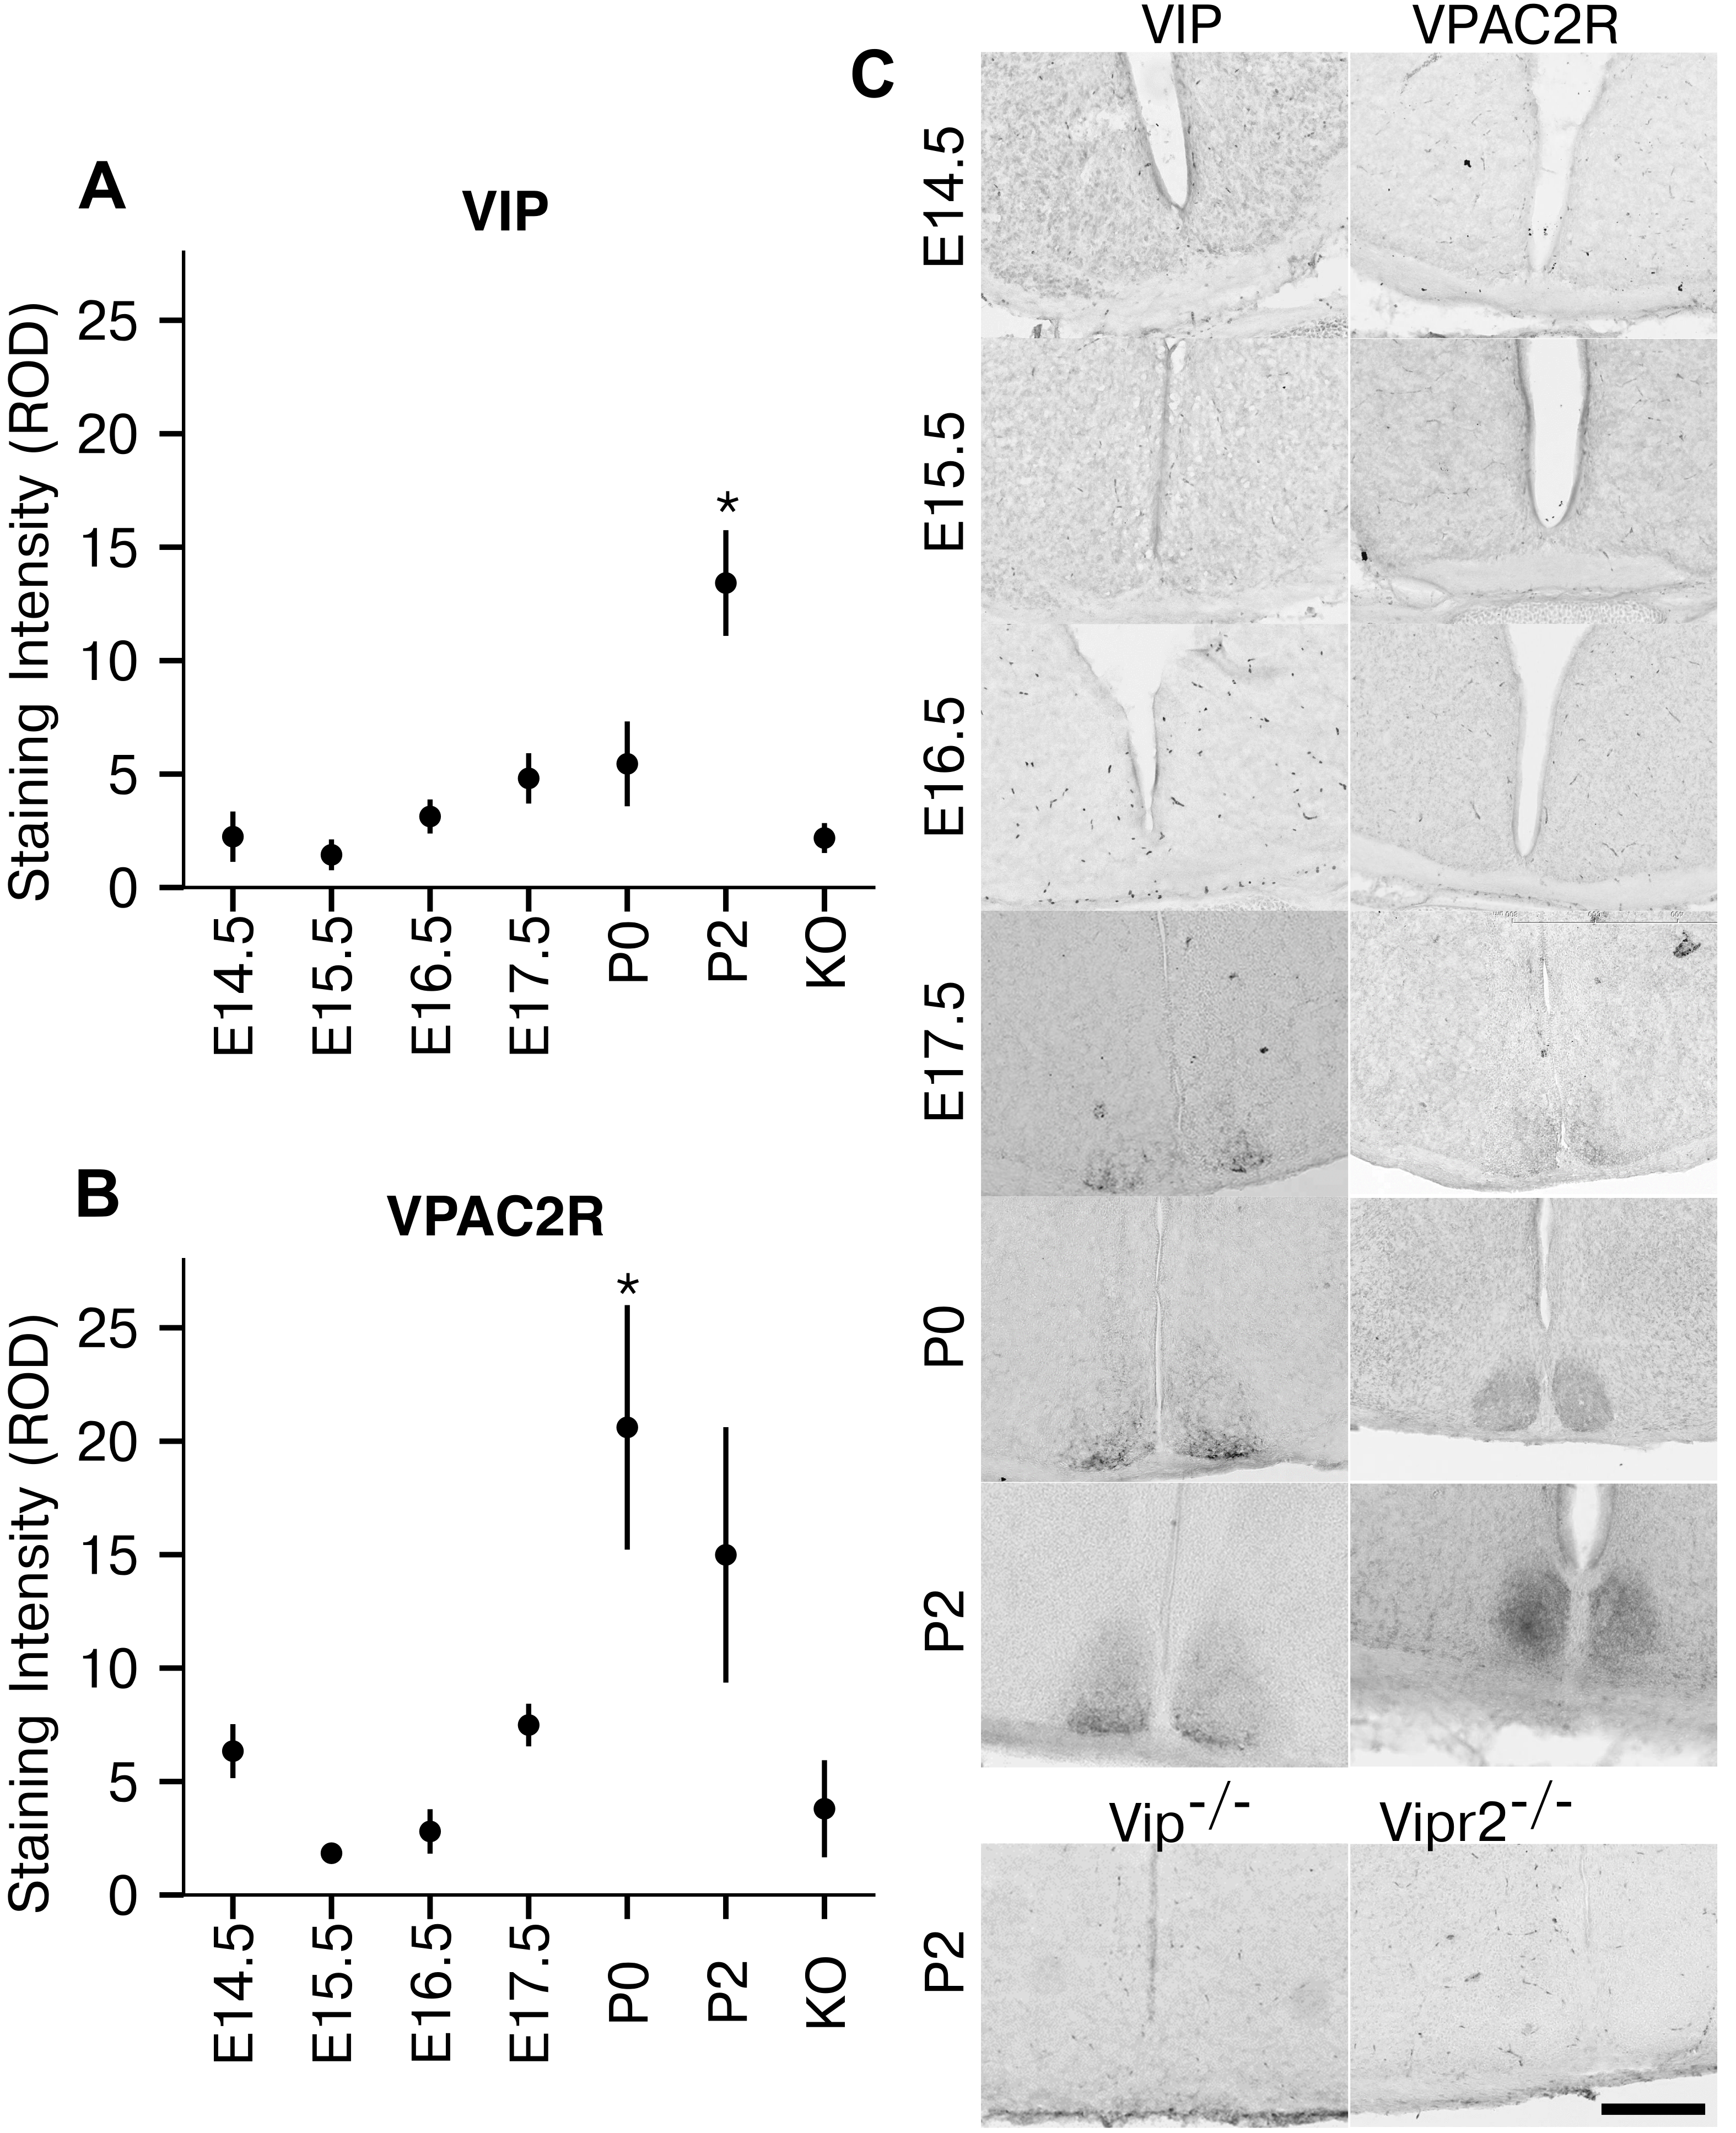
\includegraphics[width=3.5in]{chap4/figures/Figure6.png}
    \end{center}
    \caption{\label{fig:vc6} VIP and VPAC2R expression matured in the postnatal SCN. (\textbf{A}) Immunostaining intensity (Mean relative optical density $\pm$ SEM, n=9, 5, 7, 6, 7 and 7 brains at each age, respectively) of VIP in the SCN was significant by P2 compared to Vip-knockout controls (n=5, *P < 0.05, one-way ANOVA with Tukey’s HSD). (\textbf{B}) Immunostaining intensity (Mean ± SEM) of VPAC2R (n=6, 6, 5, 5, 7, and 6 brains, respectively) was significant by P0 compared to Vipr2-knockout controls (n=5, *P<0.05, one-way ANOVA with Tukey’s HSD). (\textbf{C})  Representative coronal SCN sections show the VIP (left panel) and VPAC2R (right panel) immunoreactivity at different ages. Scale bar = 200 $\mu$m.
    }
\end{figure}


\begin{figure}[!p]
    \begin{center}
        \includegraphics[width=6.5in]{chap4/figures/Figure7.png}
    \end{center}
    \caption{\label{fig:vc7} Antagonists of GABA or VIP signaling, gap junctions or neuronal firing did not disrupt circadian synchrony in the developing SCN. Drugs applied during the first day of culture of E15.5 SCN explants did not change (\textbf{A}) the fraction of pixels with circadian \textit{Per2}$^{Luc}$ (grey bars show the means across all SCN recorded at each developmental stage), or (\textbf{B}) the mean sync index over the 5 days of recording. (\textbf{C}) The synchronization index within a representative cultured E15.5 SCN treated with Veh (Vehicle), Gz (100 $\mu$M Gabazine), MEC (10 $\mu$M Meclofenamic acid), VIP antagonist (200 nM PG-99465), or TTX (2.5  $\mu$M tetrodotoxin).
    }
\end{figure}

\clearpage
\section{Discussion}

Our results indicate that E15.5 is a critical time in the maturation of the SCN.
The clock gene, PER2, is first expressed on E14.5 in the SCN and approximately 10\% of these SCN cells are weakly circadian.
By E15.5, nearly all cells within the SCN show circadian oscillation in gene expression.
Previous studies have identified E15.5 as the end of neurogenesis \cite{Shimada1973, Kabrita2008, Shimogori2010}, and transcription factors Lhx1 and ROR$\alpha$ are widely expressed across the SCN \cite{VanDunk2011}.
In particular, ROR$\alpha$ deserves further study, as it is known to be a core component of the mammalian circadian oscillator.
ROR$\alpha$ is a positive regulator of \textit{Bmal1} expression \cite{Sato2004}, and \textit{Bmal1} is an essential transcription factor and activator of \textit{Per} gene expression \cite{Hastings2014, Takahashi2016}.
ROR$\alpha$ knockout adult mice showed slight behavioral abnormalities in circadian rhythms.
We therefore speculate that expression of ROR$\alpha$ or another transcription factor in the SCN at E15.5 induces the onset of autonomous circadian oscillations in SCN cells.

Consistent with a prior publication \cite{Landgraf2015}, we found no evidence that development occurs \textit{in vitro}: on average we did not find increases in the number of oscillatory cells or SCN-wide synchrony as a recording progressed.
For example, SCN explanted on 13.5 were arrhythmic and did not show an increase in the fraction of rhythmic pixels over the course of the experiment.
SCN isolated at E14.5 or E15.5 similarly did not show changes in the amplitude, period, variability or fraction of circadian cells during 7-day recording.
Although we cannot rule out that arrhythmic, fetal SCN cells cultured longer than 7 days might develop daily cycling, our results indicate that the transition from arrhythmic to circadian is rapid and likely requires signals from outside the fetal SCN.
Other studies have found that stem cells exhibit autonomous oscillations after inducing differentiation with retinoic acid \cite{Yagita2010, Inada2014}.
Our result suggest that this signal, if it indeed initiates oscillation, does not originate spontaneously within the SCN.

Interestingly, we found that PER2 was first expressed outside the SCN.
At E14.5, extra-SCN PER2 expression was high and occasionally circadian, but was nearly completely eliminated by E15.5. 
It is not clear whether these PER2-expressing cells move into the SCN or remain in the dorsal hypothalamus while reducing their PER2 expression.
Anecdotally, it appeared that neuronal migration into the SCN region may explain this extra-SCN PER2 expression.
Further study with more rapid imaging than 1/hr would be needed to examine this possibility.
Still, rhythmic bioluminescence in these extra-SCN regions could explain the discrepancy between previous studies reporting the onset of PER2 daily oscillations in hypothalamic explants at E13 or E15 \cite{Wreschnig2014, Landgraf2015}.
The correlations between increasing fraction of rhythmic cells, increasing circadian period, and increasing period precision during this time could reflect the consequences of cell-cell communication \cite{Webb2009} or differential expression of molecular components of the circadian oscillator \cite{VanDunk2011, Ono2016}.
Together, these data support the onset of cell-autonomous circadian oscillation between E14.5 and E15.5, with intercellular communication developing shortly thereafter.

The SCN in adult mice displays a dorsal to ventral phase wave in clock gene expression \cite{Yan2002, Quintero2003, Yamaguchi2003, Evans2011a}.
Because this phase wave is not a fixed property  (e.g., it can adopt a different pattern after a temperature manipulation \textit{in vitro}) \cite{Jeong2016}, it is important to consider whether the results from the isolated SCN reflect its \textit{in vivo} circadian properties, or are simply reflective of its environment.
Our results indicate that under the constant conditions we employed, the SCN phase wave first appears after birth.
SCN explant procedures were performed at identical times of day, so although surgery has been shown to strongly reset circadian phase \cite{Wreschnig2014, Landgraf2015}, it is unlikely to cause spatial wave seen in the more mature SCN.
Furthermore, it is unlikely that surgery can start circadian oscillation in cells lacking critical clock components, as demonstrated by the lack of oscillation on E13.5 and E14.5.
Postnatal maturation of the SCN network likely involves synaptogenesis to allow direct neurotransmission.
Synaptogenesis peaks near P2, corresponding to the time at which we first found the core-shell phase wave \cite{Bedont2015}.
This provides indirect evidence, therefore, that synaptic network topology contributes to the core-shell differentiation and the phase relationships among SCN cells \cite{Abel2016, Buijink2016}.
I speculate that neurotransmission for synchrony might be undirected before synaptogenesis, and then may be synaptic in postnatal days.
The directed nature of neurotransmission through synapses would then enable the phase wave to develop, as there could then be distinct classes of neurons ``sending'' or ``receiving'' neurotransmission to establish synchrony.

Though the network continues to mature after birth, we found that SCN intercellular synchrony is established before synaptogenesis peaks.
Surgeries can reset SCN rhythms \cite{Landgraf2015}, and we found that synchrony of E14.5 and immature E15.5 SCN decreased over the course of the recording, indicating weak or no spontaneous synchronization between cells.
Intuitively, prior studies have also related increases in period variability with lower intercellular synchrony \cite{Honma2004, Webb2009}.
Our data likewise showed an increase in synchrony by E15.5 (Fig.
\ref{fig:vc3}) that corresponded with a decrease in cycle-to-cycle period variability.
This synchrony in adults is at least in part established by the neurotransmitter VIP and its receptor VIPR2 \cite{Harmar2002, Colwell2003, Aton2005, Maywood2006, Ciarleglio2009}.
In rats, \textit{Vip} mRNA is detected by E18 \cite{Ban1997, Houdek2014}, but VIP protein expression has only been examined postnatally \cite{Herzog2000}.
Our results showed that VIP protein is undetectable by immunochemistry before birth.
While this may seem startling, this result corresponds well with a prior study in which embryonic SCN explants from VIP$^{-/-}$ mice maintained circadian oscillations at the tissue level \cite{Wreschnig2014}, indicative of intercellular synchrony.
Our results further demonstrate that synchrony is achieved near E15.5, at least several days before significant expression of VIP or its receptor VIPR2.
Finally, that VIP antagonist does not interfere with synchrony or cell-autonomous oscillation suggests that other neural signals are sufficient to sustain synchrony before the maturation of the SCN. 

The increase in synchrony in the SCN at E15.5 does coincide with Lhx1 expression across the SCN \cite{VanDunk2011}.
This transcription factor is important for the expression of diverse neuropeptide coupling signals aside from VIP, such as GRP or AVP \cite{Bedont2014}.
Because these signals can mediate the synchrony in adults \cite{Brown2005, Maywood2011} and in postnatal ages \cite{Ono2016}, they are candidates for sustaining spontaneous SCN synchrony during embryonic development.

It has long been recognized that the accumulation of intercellular calcium, through opening voltage-gated Ca$^{2+}$ channels during action potentials, is the trigger for neurotransmitter release \cite{Rubin1970,Shin2003}.
In this chapter, we did not seek to determine the onset of neuronal firing within the SCN, or its interaction with the expression or release of small neurotransmitters such as GABA or large neuropeptides such as VIP \cite{Buijs1995}.
This interaction is compounded by the release of VIP from large dense-core vesicles, rather than the relatively well-understood small clear-core vesicles \cite{Salio2006}.
This topic would make for an interesting follow-up study, as it would shed light on the role of membrane potential in cell-autonomous and tissue circadian rhtyhms, as well as on neurotransmitter and neuropeptide release more broadly.
For example, it is unclear if neuronal excitability should be considered a clock output, input, or core feature.
In the following chapter, we begin to address these open questions by identifying firing patterns within the mature SCN, and how these firing patterns relate to neuronal class as determined by VIP expression.












\include{chap5/mazuski}
\chapter{Summary and future directions: preliminary and proposed studies of circadian control}

The prior two chapters have presented preliminary theoretical studies of circadian control.
The first result, a comparison of optimal with model predictive control, presents an important benchmark for the performance of any applied control scheme, and uses this to identify how MPC design parameters affect control optimality.
The second result proposes a method for controlling populations of oscillators without adversely affecting population synchrony.
While these propose a path toward translational closed-loop circadian control, there are remaining challenges before either may be implemented.

Herein, I briefly discuss future research directions toward the control of circadian rhythms.
The first of these is the development of a real-time sensor of circadian phase, an essential development for circadian control in ambulatory conditions.
The second proposed direction involves improving control abilities by relaxing the assumption that the oscillator stays near its limit cycle.
By relaxing this assumption, we may shift the oscillator closer to its fixed point, where phases are more condensed in state space, and therefore may be shifted between more easily.

\section{Closing the loop: development of a circadian phase sensor}

Although we have made significant progress in developing control algorithms for circadian oscillation, there remains significant barriers to achieving closed-loop control in clinical settings.
Most prominently, there is little current capability for real-time sensing of circadian phase, and even less ability when invasive or expensive methods are excluded.
Open loop control does not require sensing of phase, and therefore it has been used exclusively to-date in publicly available phase resetting protocols \cite{Walch2016}.
The ability of feedback control to overcome imprecise modeling and poor model assumptions arises directly from the incorporation of feedback, and so sensing phase is an essential component of more advanced control systems.
In clinical settings, circadian phase is generally assessed by salivary or blood melatonin levels, core body temperature (as recorded from a rectal thermometer), or, rarely, cortisol levels \cite{Klerman2002, Chang2012a, StHilaire2012}.
While these techniques allow precise phase calculations in clinic, they are insufficient for ambulatory settings and prohibitively invasive for widespread adoption.

There has been a recent push to use machine learning techniques to sense circadian phase from ambulatory data; for example, recent studies have combined skin temperature sensors and actigraphy recordings to estimate phase \cite{Kolodyazhniy2011, Kolodyazhniy2012}.
Machine learning methods have shown promise and improved performance in comparison simple multiple regression models, with the majority of phase estimates within $\pm0.3$ radians (approximately 1 h).
In these cases, the actigraphy recordings provided little utility in comparison to the skin temperature sensors \cite{Kolodyazhniy2012}.
However, actigraphy data is the most readily available to the average individual through motion sensing in smartphones or smartwatches.
An improved approach might include sampling the individual's ambient light environment in addition to activity.
Data of this sort have already been collected by the Klerman lab at Harvard Medical School/Brigham and Women's Hospital from a cohort of approximately 150 college undergraduates.
A logical next step would be using machine learning to estimate continuous phase from this dataset, and compare with clinical phase measurements.

A potentially helpful approach in linking the sensor to the control algorithm would be the use of a confidence index, a scalar metric describing the historical accuracy of phase prediction given the input data \cite{Laguna2017}.
In this case, the confidence index could indicate a high degree of certainty in the estimated phase, or if the confidence in phase estimation is low, a high degree of certainty regarding the predicted response (i.e.\ if all likely phases result in the same phase shift).
This metric would then be used to tune the aggressiveness of the controller or the sampling rate.
A simple confidence index would, for example, stop control action when in the vicinity of ipPRC zero crosses, to prevent accidentally shifting the phase in the non-optimal direction.
Approaches such as those in Chapter 6 could be used to similarly find bounds on the error incurred due to imprecision in the phase estimation, and these calculations would dictate how the confidence index would be incorporated into the controller.

When combined with the MPC approaches from the prior two chapters, the development of a phase sensor will enable the first closed-loop control of circadian phase.
Though there are no current plans to perform closed-loop human circadian control experiments, I anticipate that closed-loop circadian control will be feasible in a clinical setting within the next five years.
Aside from circadian control, the ability to sense circadian phase has potential benefits in other aspects of precision medicine.
For example, the majority of common pharmaceuticals target clock products, and circadian phase affects the pharmacokinetic and pharmacodynamic properties of nearly any therapeutic, since RNA abundance of about 40\% of protein-coding genes are thought to cycle with a circadian rhythm \cite{Zhang2014a}.
Thus, the ability to accurately and noninvasively assess circadian phase is critical for the development of next-generation dynamic drug delivery strategies.

\section{Critical-resetting MPC: leveraging the limit-cycle fixed point}

\subsection*{Introduction}
When developing controls methods for manipulating circadian phase, we made the decision to reduce the limit-cycle oscillator model to a phase-only formulation.
In doing so, we reduced the dimensionality of state space from $n$ dimensions to a single dimension.
This allowed simple use of the phase response curve to identify when the oscillator would be phase-delayed or phase-advanced by the stimulus.
We applied control based off the ipPRC we calculated, and referred to such a PRC as ``type 1.''
For large perturbations, or in some cases repeated perturbations \cite{Kronauer1999}, a ``type 0'' PRC has also been observed \cite{Czeisler1989}.
A type 0 PRC (called so because the mean slope of the phase transition curve, or PTC, is 0) contains a discontinuity resulting from the large magnitude phase shifts it describes.
This discontinuity mathematically arises from the oscillator being shifted far from the limit cycle in state space, and as a result, only having access to a subset of all possible final phases.

Type 0 resetting that results from the oscillator being pushed close to the critical point (from here, called ``critical resetting'') has an additional feature: a sustained reduction in the amplitude of circadian processes such as melatonin or core body temperature rhythms, which reverts to the pre-stimulus amplitude very slowly \cite{Jewett1994, Kronauer1999}.
The critical point is without phase, and correspondingly, individuals that have been shifted sufficiently near this point may be easily phase shifted into any desirable final phase.
Thus, it is feasible to design a ``critical MPC'' protocol for achieving large phase shifts by first forcing the individual to the critical point, then aligning them with the desired final phase.
However, this violates the phase-only assumption of the prior chapters.

A further to-date unexplained curiosity from these early studies of human circadian phase and amplitude resetting is that only a fraction ($\approx25$\%) of individuals respond to an identical series of stimuli with a critical resetting.
The preliminary work in this section sought to first explain this result, and in doing so, determine if critical resetting may be more widely achieved and used in circadian control. 


\subsection*{Modeling light input to the human circadian oscillator}

The most widely-used model of the circadian clock was developed by Kronauer and his collaborators nearly two decades ago \cite{Jewett1998,Kronauer1999}.
This model incorporates two processes.


Process P is a limit cycle oscillator, modified from the van der Pol oscillator, intended to capture endogenous circadian oscillation.
The two states of process P are given by:
\begin{equation}
    \frac{dX}{dt} = \left(\frac{\pi}{12}\right)\left(X_c + \mu \bigg(\frac{1}{3}X + \frac{4}{3}X^3 - \frac{256}{105}X^7\bigg) +B(t)\right) 
\end{equation}
\begin{equation}
    \frac{dX_c}{dt} =\left(\frac{\pi}{12}\right)\left(qB(t)\bigg(\frac{24}{0.99729\tau}\bigg)^2 X_c X + kB(t)X\right)
\end{equation}
where $X$ represents core body temperature, and $X_c$ is a non-biological co-state that drives oscillation.
Parameter $\tau$, here, is the period of oscillation, which may be selected \textit{a priori} and is typically set to $24.2$ h, to correspond with the human circadian period \cite{Czeisler1999}.
The kinetic parameters $\mu$, $q$, and $k$ do not have biological significance beyond parameterizing the shape of the limit cycle and are given in \cite{Kronauer1999}.
Term $B(t)$ is the photic drive, which is determined by process L.

Process L describes the dynamic effect of light input into the oscillator.
Experiments where light pulses were applied for varying durations and with varying spacing have shown that light response is pseudosaturating.
That is, the initial response to the pulse evokes a large-magnitude shift.
Continuing the light stimulus for a longer duration yields diminishing returns, until a constant, low level of drive is reached.
This response can be captured by modeling the dynamics of a population of light receptors, where $n(t)$ are the fraction of the population that is inactive, and $1-n(t)$ are active.
The conversion between active and inactive states is given by
\begin{equation}
    \frac{dn}{dt} = 60(\alpha(t)(1-n) - \beta n)
\end{equation}
where $\alpha$ and $\beta$ are the kinetic rates of inactivation and activation, respectively.
Thus, after a constant, sustained pulse, the fraction of the population that is active is given by $n_\infty = \alpha/(\alpha+\beta)$, yielding the pseudosaturation.
The kinetic term $\alpha$ is a function of light intensity, given by
\begin{equation}
    \alpha(t) = \alpha_0 \left(\frac{I}{I_0}\right)^p.
\end{equation}
The light drive from the receptors, $\hat B(t)$, is then a function of light intensity and the fraction of active states:
\begin{equation}
    \hat B(t) = G\alpha(t)(1-n(t)).
\end{equation}
Because the clock is more sensitive to light at certain phases, $\hat B$ is rescaled by the photic sensitivity state of the oscillator, to yield the effective light drive term $B(t)$:
\begin{equation}
    B(t) = (1-0.4X)(1-0.4X_c)\hat B(t),
\end{equation}
which is incorporated in process P.
The techniques used for fitting this model are explained in detail in \cite{Kronauer1999}.

Importantly, this model was fit to exhibit critical resetting in response to three five-hour pulses centered at the core body temperature ($X$) minimum (corresponding to approximately 5AM local time).

\subsection*{Inter-individual period variability explains critical resetting prevalence}

\begin{figure}[p]
    \begin{center}
        \includegraphics[width=6.5in]{chap10/figures/blind.png}
    \end{center}
        \caption{\label{fig:blind} Simulation of the three pulse experiment from \cite{Kronauer1999} demonstrates effect of period on critical resetting.
    Periods that are short (\textbf{A}) or long (\textbf{C}) do not reach the critical point, whereas an intermediate value (\textbf{B}) yields a trajectory that very nearly approaches the critical point.}
\end{figure}

\begin{figure}[p]
    \begin{center}
        \includegraphics[width=3.5in]{chap10/figures/threepulse_sensitivity.png}
    \end{center}
        \caption{\label{fig:blind2} Simulation of the three pulse experiment from \cite{Kronauer1999} yields a plot of distance from the critical point for a range of individual periods ($\tau$).}
\end{figure}

Core body temperature minimum corresponds to the positive zero-cross of the type 1 PRC for this model (see Figure 11 in \cite{Kronauer1999}).
The critical resetting protocol (three 5-h pulses of 9500 lux 19 h apart, centered at core body temperature minimum on the first day) is therefore highly sensitive to period variability.
If the oscillatory period is too short, the 5 h pulse will occur primarily after the minimum, in the phase advance region.
This would result in the ensuing core body temperature minimum occurring even earlier due to the phase advance, and the ensuing pulse falling further into the phase advance region each time, and missing the timing that results in a critical resetting.
Likewise, if the period is too long, the pulse will be applied primarily before the minimum, incurring phase delays.
The minimum will occur later each each day, and the pulse will not be delayed, resulting in also missing the core body temperature minimum.

Three simulation examples of the three-pulse experiment are shown in Figure \ref{fig:blind}, demonstrating the effect of short period (\ref{fig:blind}A), ``just right'' period (\ref{fig:blind}B), and long period (\ref{fig:blind}C) responses to the protocol.
Human period is near 24.2 h, but varies between individuals ($24.18 \pm 0.13$ mean $\pm$ standard deviation \cite{Czeisler1999}), and so this may explain why only some individuals achieve a critical reset.

To test this further, I performed this simulation for a range of $\tau$ values and plotted the distance to the critical point following the third pulse (Figure \ref{fig:blind2}).
The results show that slight changes in the period drastically alter the timing of each pulse, and thus the final distance to the critical point.
Importantly, the ``perfect'' predicted period for achieving a critical resetting ($\approx 24.6$ h) is dependent on the whole model parameterization in addition to $\tau$, and therefore may not exactly correspond to that observed in humans.
However, I predict that the general trend will be the same: the damping of amplitudes indicative of a critical resetting will be a function of individual period, with both long and short periods unable to reach the critical point.


\subsection*{A simple feedback control scheme to achieve critical resetting}
\afterpage{
\begin{figure}[p]
    \begin{center}
        \includegraphics[width=6.5in]{chap10/figures/ctrl.png}
    \end{center}
        \caption{\label{fig:ctrl3} Simulation of the three pulse experiment from \cite{Kronauer1999} under closed-loop control.
    Oscillators with periods that are short (\textbf{A}) or long (\textbf{C}) are now able to reach the critical point comparably to that with the ``ideal'' period length of 24.6 h (\textbf{B}).}
\end{figure}
\clearpage
\begin{figure}[p]
    \begin{center}
        \includegraphics[width=3.5in]{chap10/figures/comparison.png}
    \end{center}
        \caption{\label{fig:ctrl32} Simulation of the three pulse experiment from \cite{Kronauer1999} either shooting blind (open-loop) or under closed-loop control yields a plot of distance from the critical point for a range of individual periods ($\tau$). Notably, the distance to the critical point is reduced in all cases.}
\end{figure}
}

Achieving a critical reset is desirable for the ability to return to the limit cycle at any phase following the resetting.
The prior result suggests that simply applying the three light pulses under feedback control would allow targeting of the core body temperature minimum, even if it were to shift following a light pulse.
This would enable critical resetting even in individuals that could not achieve it under open loop (i.e. no feedback) application of light.
Here, I tested that prediction.

To do so, I first identified the phase at which the light pulse begins for the optimal individual period ($\tau = 24.6$ h).
This phase was found to be approximately 2.66 radians, and denoted $\phi_{\text{start}}$.
I then performed feedback control simulations where the phase was calculated every 30 minutes.
When the measured phase first exceeded $\phi_{\text{start}}$, the 5 h pulse was applied.
Phase tracking resumed following the pulse. 

Figures \ref{fig:ctrl3} and \ref{fig:ctrl32} demonstrate the results of the three pulse experiment now under feedback control.
Because the application of light is now performed in closed-loop, a critical resetting is achieved irrespective of long or short oscillatory periods (Figure \ref{fig:ctrl3}A,C).
Furthermore, any oscillator with a period within physiological range is predicted to approach the critical point under closed-loop control (Figure \ref{fig:ctrl32}).


These very encouraging results warrant further examination, and work is currently underway to (i) design a feedback control protocol based on amplitude response curves rather than phase comparison, and (ii) determine if it is feasible to implement such a strategy in a clinical or ambulatory setting.
Toward aim (i), the infinitesimal parametric amplitude response curve can be calculated for this model for the light input (term $B(t)$).
This might allow us to better guide the delivery of light based on properties of the oscillator, rather than simply relying on repeating a clinical protocol. 
In approaching aim (ii), the essential element for implementing this protocol is the ability to sense phase sufficiently accurately for achieving a critical reset.
A first step, then, would be examining exactly how sensitive critical resetting is to mistimed application of the light pulse due to imprecisions in on-line phase sensing.
The controller, as currently formulated, applies feedback within a half hour of the desired phase.
This is sufficient to achieve critical resetting, as errors do not compound from cycle-to-cycle, unlike the open loop case.

\section{Conclusion}
In sum, closed-loop circadian control is a relatively unexplored problem at the interface of control theory and systems biology. 
Whether by incurring incremental shifts via a pharmaceutical stimulus, or by exploiting the oscillatory critical point, circadian control has the potential to improve quality of life for shift workers or any individual attempting to maximize cognitive or physical performance. 
Though significant challenges remain in implementing closed-loop circadian control, the technology to do so exists.
It is my hope that the research contained in this dissertation is an incremental step in the direction of understanding and control over the circadian rhythms that affect nearly every living organism.















\part{Control of the Mammalian Circadian Oscillator}
\include{chap6/mpc}
\include{chap7/emerging}
\chapter{Summary and future directions: preliminary and proposed studies of circadian control}

The prior two chapters have presented preliminary theoretical studies of circadian control.
The first result, a comparison of optimal with model predictive control, presents an important benchmark for the performance of any applied control scheme, and uses this to identify how MPC design parameters affect control optimality.
The second result proposes a method for controlling populations of oscillators without adversely affecting population synchrony.
While these propose a path toward translational closed-loop circadian control, there are remaining challenges before either may be implemented.

Herein, I briefly discuss future research directions toward the control of circadian rhythms.
The first of these is the development of a real-time sensor of circadian phase, an essential development for circadian control in ambulatory conditions.
The second proposed direction involves improving control abilities by relaxing the assumption that the oscillator stays near its limit cycle.
By relaxing this assumption, we may shift the oscillator closer to its fixed point, where phases are more condensed in state space, and therefore may be shifted between more easily.

\section{Closing the loop: development of a circadian phase sensor}

Although we have made significant progress in developing control algorithms for circadian oscillation, there remains significant barriers to achieving closed-loop control in clinical settings.
Most prominently, there is little current capability for real-time sensing of circadian phase, and even less ability when invasive or expensive methods are excluded.
Open loop control does not require sensing of phase, and therefore it has been used exclusively to-date in publicly available phase resetting protocols \cite{Walch2016}.
The ability of feedback control to overcome imprecise modeling and poor model assumptions arises directly from the incorporation of feedback, and so sensing phase is an essential component of more advanced control systems.
In clinical settings, circadian phase is generally assessed by salivary or blood melatonin levels, core body temperature (as recorded from a rectal thermometer), or, rarely, cortisol levels \cite{Klerman2002, Chang2012a, StHilaire2012}.
While these techniques allow precise phase calculations in clinic, they are insufficient for ambulatory settings and prohibitively invasive for widespread adoption.

There has been a recent push to use machine learning techniques to sense circadian phase from ambulatory data; for example, recent studies have combined skin temperature sensors and actigraphy recordings to estimate phase \cite{Kolodyazhniy2011, Kolodyazhniy2012}.
Machine learning methods have shown promise and improved performance in comparison simple multiple regression models, with the majority of phase estimates within $\pm0.3$ radians (approximately 1 h).
In these cases, the actigraphy recordings provided little utility in comparison to the skin temperature sensors \cite{Kolodyazhniy2012}.
However, actigraphy data is the most readily available to the average individual through motion sensing in smartphones or smartwatches.
An improved approach might include sampling the individual's ambient light environment in addition to activity.
Data of this sort have already been collected by the Klerman lab at Harvard Medical School/Brigham and Women's Hospital from a cohort of approximately 150 college undergraduates.
A logical next step would be using machine learning to estimate continuous phase from this dataset, and compare with clinical phase measurements.

A potentially helpful approach in linking the sensor to the control algorithm would be the use of a confidence index, a scalar metric describing the historical accuracy of phase prediction given the input data \cite{Laguna2017}.
In this case, the confidence index could indicate a high degree of certainty in the estimated phase, or if the confidence in phase estimation is low, a high degree of certainty regarding the predicted response (i.e.\ if all likely phases result in the same phase shift).
This metric would then be used to tune the aggressiveness of the controller or the sampling rate.
A simple confidence index would, for example, stop control action when in the vicinity of ipPRC zero crosses, to prevent accidentally shifting the phase in the non-optimal direction.
Approaches such as those in Chapter 6 could be used to similarly find bounds on the error incurred due to imprecision in the phase estimation, and these calculations would dictate how the confidence index would be incorporated into the controller.

When combined with the MPC approaches from the prior two chapters, the development of a phase sensor will enable the first closed-loop control of circadian phase.
Though there are no current plans to perform closed-loop human circadian control experiments, I anticipate that closed-loop circadian control will be feasible in a clinical setting within the next five years.
Aside from circadian control, the ability to sense circadian phase has potential benefits in other aspects of precision medicine.
For example, the majority of common pharmaceuticals target clock products, and circadian phase affects the pharmacokinetic and pharmacodynamic properties of nearly any therapeutic, since RNA abundance of about 40\% of protein-coding genes are thought to cycle with a circadian rhythm \cite{Zhang2014a}.
Thus, the ability to accurately and noninvasively assess circadian phase is critical for the development of next-generation dynamic drug delivery strategies.

\section{Critical-resetting MPC: leveraging the limit-cycle fixed point}

\subsection*{Introduction}
When developing controls methods for manipulating circadian phase, we made the decision to reduce the limit-cycle oscillator model to a phase-only formulation.
In doing so, we reduced the dimensionality of state space from $n$ dimensions to a single dimension.
This allowed simple use of the phase response curve to identify when the oscillator would be phase-delayed or phase-advanced by the stimulus.
We applied control based off the ipPRC we calculated, and referred to such a PRC as ``type 1.''
For large perturbations, or in some cases repeated perturbations \cite{Kronauer1999}, a ``type 0'' PRC has also been observed \cite{Czeisler1989}.
A type 0 PRC (called so because the mean slope of the phase transition curve, or PTC, is 0) contains a discontinuity resulting from the large magnitude phase shifts it describes.
This discontinuity mathematically arises from the oscillator being shifted far from the limit cycle in state space, and as a result, only having access to a subset of all possible final phases.

Type 0 resetting that results from the oscillator being pushed close to the critical point (from here, called ``critical resetting'') has an additional feature: a sustained reduction in the amplitude of circadian processes such as melatonin or core body temperature rhythms, which reverts to the pre-stimulus amplitude very slowly \cite{Jewett1994, Kronauer1999}.
The critical point is without phase, and correspondingly, individuals that have been shifted sufficiently near this point may be easily phase shifted into any desirable final phase.
Thus, it is feasible to design a ``critical MPC'' protocol for achieving large phase shifts by first forcing the individual to the critical point, then aligning them with the desired final phase.
However, this violates the phase-only assumption of the prior chapters.

A further to-date unexplained curiosity from these early studies of human circadian phase and amplitude resetting is that only a fraction ($\approx25$\%) of individuals respond to an identical series of stimuli with a critical resetting.
The preliminary work in this section sought to first explain this result, and in doing so, determine if critical resetting may be more widely achieved and used in circadian control. 


\subsection*{Modeling light input to the human circadian oscillator}

The most widely-used model of the circadian clock was developed by Kronauer and his collaborators nearly two decades ago \cite{Jewett1998,Kronauer1999}.
This model incorporates two processes.


Process P is a limit cycle oscillator, modified from the van der Pol oscillator, intended to capture endogenous circadian oscillation.
The two states of process P are given by:
\begin{equation}
    \frac{dX}{dt} = \left(\frac{\pi}{12}\right)\left(X_c + \mu \bigg(\frac{1}{3}X + \frac{4}{3}X^3 - \frac{256}{105}X^7\bigg) +B(t)\right) 
\end{equation}
\begin{equation}
    \frac{dX_c}{dt} =\left(\frac{\pi}{12}\right)\left(qB(t)\bigg(\frac{24}{0.99729\tau}\bigg)^2 X_c X + kB(t)X\right)
\end{equation}
where $X$ represents core body temperature, and $X_c$ is a non-biological co-state that drives oscillation.
Parameter $\tau$, here, is the period of oscillation, which may be selected \textit{a priori} and is typically set to $24.2$ h, to correspond with the human circadian period \cite{Czeisler1999}.
The kinetic parameters $\mu$, $q$, and $k$ do not have biological significance beyond parameterizing the shape of the limit cycle and are given in \cite{Kronauer1999}.
Term $B(t)$ is the photic drive, which is determined by process L.

Process L describes the dynamic effect of light input into the oscillator.
Experiments where light pulses were applied for varying durations and with varying spacing have shown that light response is pseudosaturating.
That is, the initial response to the pulse evokes a large-magnitude shift.
Continuing the light stimulus for a longer duration yields diminishing returns, until a constant, low level of drive is reached.
This response can be captured by modeling the dynamics of a population of light receptors, where $n(t)$ are the fraction of the population that is inactive, and $1-n(t)$ are active.
The conversion between active and inactive states is given by
\begin{equation}
    \frac{dn}{dt} = 60(\alpha(t)(1-n) - \beta n)
\end{equation}
where $\alpha$ and $\beta$ are the kinetic rates of inactivation and activation, respectively.
Thus, after a constant, sustained pulse, the fraction of the population that is active is given by $n_\infty = \alpha/(\alpha+\beta)$, yielding the pseudosaturation.
The kinetic term $\alpha$ is a function of light intensity, given by
\begin{equation}
    \alpha(t) = \alpha_0 \left(\frac{I}{I_0}\right)^p.
\end{equation}
The light drive from the receptors, $\hat B(t)$, is then a function of light intensity and the fraction of active states:
\begin{equation}
    \hat B(t) = G\alpha(t)(1-n(t)).
\end{equation}
Because the clock is more sensitive to light at certain phases, $\hat B$ is rescaled by the photic sensitivity state of the oscillator, to yield the effective light drive term $B(t)$:
\begin{equation}
    B(t) = (1-0.4X)(1-0.4X_c)\hat B(t),
\end{equation}
which is incorporated in process P.
The techniques used for fitting this model are explained in detail in \cite{Kronauer1999}.

Importantly, this model was fit to exhibit critical resetting in response to three five-hour pulses centered at the core body temperature ($X$) minimum (corresponding to approximately 5AM local time).

\subsection*{Inter-individual period variability explains critical resetting prevalence}

\begin{figure}[p]
    \begin{center}
        \includegraphics[width=6.5in]{chap10/figures/blind.png}
    \end{center}
        \caption{\label{fig:blind} Simulation of the three pulse experiment from \cite{Kronauer1999} demonstrates effect of period on critical resetting.
    Periods that are short (\textbf{A}) or long (\textbf{C}) do not reach the critical point, whereas an intermediate value (\textbf{B}) yields a trajectory that very nearly approaches the critical point.}
\end{figure}

\begin{figure}[p]
    \begin{center}
        \includegraphics[width=3.5in]{chap10/figures/threepulse_sensitivity.png}
    \end{center}
        \caption{\label{fig:blind2} Simulation of the three pulse experiment from \cite{Kronauer1999} yields a plot of distance from the critical point for a range of individual periods ($\tau$).}
\end{figure}

Core body temperature minimum corresponds to the positive zero-cross of the type 1 PRC for this model (see Figure 11 in \cite{Kronauer1999}).
The critical resetting protocol (three 5-h pulses of 9500 lux 19 h apart, centered at core body temperature minimum on the first day) is therefore highly sensitive to period variability.
If the oscillatory period is too short, the 5 h pulse will occur primarily after the minimum, in the phase advance region.
This would result in the ensuing core body temperature minimum occurring even earlier due to the phase advance, and the ensuing pulse falling further into the phase advance region each time, and missing the timing that results in a critical resetting.
Likewise, if the period is too long, the pulse will be applied primarily before the minimum, incurring phase delays.
The minimum will occur later each each day, and the pulse will not be delayed, resulting in also missing the core body temperature minimum.

Three simulation examples of the three-pulse experiment are shown in Figure \ref{fig:blind}, demonstrating the effect of short period (\ref{fig:blind}A), ``just right'' period (\ref{fig:blind}B), and long period (\ref{fig:blind}C) responses to the protocol.
Human period is near 24.2 h, but varies between individuals ($24.18 \pm 0.13$ mean $\pm$ standard deviation \cite{Czeisler1999}), and so this may explain why only some individuals achieve a critical reset.

To test this further, I performed this simulation for a range of $\tau$ values and plotted the distance to the critical point following the third pulse (Figure \ref{fig:blind2}).
The results show that slight changes in the period drastically alter the timing of each pulse, and thus the final distance to the critical point.
Importantly, the ``perfect'' predicted period for achieving a critical resetting ($\approx 24.6$ h) is dependent on the whole model parameterization in addition to $\tau$, and therefore may not exactly correspond to that observed in humans.
However, I predict that the general trend will be the same: the damping of amplitudes indicative of a critical resetting will be a function of individual period, with both long and short periods unable to reach the critical point.


\subsection*{A simple feedback control scheme to achieve critical resetting}
\afterpage{
\begin{figure}[p]
    \begin{center}
        \includegraphics[width=6.5in]{chap10/figures/ctrl.png}
    \end{center}
        \caption{\label{fig:ctrl3} Simulation of the three pulse experiment from \cite{Kronauer1999} under closed-loop control.
    Oscillators with periods that are short (\textbf{A}) or long (\textbf{C}) are now able to reach the critical point comparably to that with the ``ideal'' period length of 24.6 h (\textbf{B}).}
\end{figure}
\clearpage
\begin{figure}[p]
    \begin{center}
        \includegraphics[width=3.5in]{chap10/figures/comparison.png}
    \end{center}
        \caption{\label{fig:ctrl32} Simulation of the three pulse experiment from \cite{Kronauer1999} either shooting blind (open-loop) or under closed-loop control yields a plot of distance from the critical point for a range of individual periods ($\tau$). Notably, the distance to the critical point is reduced in all cases.}
\end{figure}
}

Achieving a critical reset is desirable for the ability to return to the limit cycle at any phase following the resetting.
The prior result suggests that simply applying the three light pulses under feedback control would allow targeting of the core body temperature minimum, even if it were to shift following a light pulse.
This would enable critical resetting even in individuals that could not achieve it under open loop (i.e. no feedback) application of light.
Here, I tested that prediction.

To do so, I first identified the phase at which the light pulse begins for the optimal individual period ($\tau = 24.6$ h).
This phase was found to be approximately 2.66 radians, and denoted $\phi_{\text{start}}$.
I then performed feedback control simulations where the phase was calculated every 30 minutes.
When the measured phase first exceeded $\phi_{\text{start}}$, the 5 h pulse was applied.
Phase tracking resumed following the pulse. 

Figures \ref{fig:ctrl3} and \ref{fig:ctrl32} demonstrate the results of the three pulse experiment now under feedback control.
Because the application of light is now performed in closed-loop, a critical resetting is achieved irrespective of long or short oscillatory periods (Figure \ref{fig:ctrl3}A,C).
Furthermore, any oscillator with a period within physiological range is predicted to approach the critical point under closed-loop control (Figure \ref{fig:ctrl32}).


These very encouraging results warrant further examination, and work is currently underway to (i) design a feedback control protocol based on amplitude response curves rather than phase comparison, and (ii) determine if it is feasible to implement such a strategy in a clinical or ambulatory setting.
Toward aim (i), the infinitesimal parametric amplitude response curve can be calculated for this model for the light input (term $B(t)$).
This might allow us to better guide the delivery of light based on properties of the oscillator, rather than simply relying on repeating a clinical protocol. 
In approaching aim (ii), the essential element for implementing this protocol is the ability to sense phase sufficiently accurately for achieving a critical reset.
A first step, then, would be examining exactly how sensitive critical resetting is to mistimed application of the light pulse due to imprecisions in on-line phase sensing.
The controller, as currently formulated, applies feedback within a half hour of the desired phase.
This is sufficient to achieve critical resetting, as errors do not compound from cycle-to-cycle, unlike the open loop case.

\section{Conclusion}
In sum, closed-loop circadian control is a relatively unexplored problem at the interface of control theory and systems biology. 
Whether by incurring incremental shifts via a pharmaceutical stimulus, or by exploiting the oscillatory critical point, circadian control has the potential to improve quality of life for shift workers or any individual attempting to maximize cognitive or physical performance. 
Though significant challenges remain in implementing closed-loop circadian control, the technology to do so exists.
It is my hope that the research contained in this dissertation is an incremental step in the direction of understanding and control over the circadian rhythms that affect nearly every living organism.
















\backmatter
{\singlespace
\bibliographystyle{myIEEEtran.bst}
\bibliography{condensed_library.bib}
%\bibliography{library.bib}
%\include{appendix/appendix}
}




\end{document}





%%% 
TO DO LIST:
- add in cristina paper (end jan)
- correct notation (end jan)
- write abstract (end feb)
- write future aims sections (end feb)

%%%















